% Options for packages loaded elsewhere
\PassOptionsToPackage{unicode}{hyperref}
\PassOptionsToPackage{hyphens}{url}
%
\documentclass[
  openany]{book}
\usepackage{lmodern}
\usepackage{amssymb,amsmath}
\usepackage{ifxetex,ifluatex}
\ifnum 0\ifxetex 1\fi\ifluatex 1\fi=0 % if pdftex
  \usepackage[T1]{fontenc}
  \usepackage[utf8]{inputenc}
  \usepackage{textcomp} % provide euro and other symbols
\else % if luatex or xetex
  \usepackage{unicode-math}
  \defaultfontfeatures{Scale=MatchLowercase}
  \defaultfontfeatures[\rmfamily]{Ligatures=TeX,Scale=1}
\fi
% Use upquote if available, for straight quotes in verbatim environments
\IfFileExists{upquote.sty}{\usepackage{upquote}}{}
\IfFileExists{microtype.sty}{% use microtype if available
  \usepackage[]{microtype}
  \UseMicrotypeSet[protrusion]{basicmath} % disable protrusion for tt fonts
}{}
\makeatletter
\@ifundefined{KOMAClassName}{% if non-KOMA class
  \IfFileExists{parskip.sty}{%
    \usepackage{parskip}
  }{% else
    \setlength{\parindent}{0pt}
    \setlength{\parskip}{6pt plus 2pt minus 1pt}}
}{% if KOMA class
  \KOMAoptions{parskip=half}}
\makeatother
\usepackage{xcolor}
\IfFileExists{xurl.sty}{\usepackage{xurl}}{} % add URL line breaks if available
\IfFileExists{bookmark.sty}{\usepackage{bookmark}}{\usepackage{hyperref}}
\hypersetup{
  pdftitle={Comprehensive Crap Guide},
  pdfauthor={Deependra Dhakal, Samita Paudel},
  hidelinks,
  pdfcreator={LaTeX via pandoc}}
\urlstyle{same} % disable monospaced font for URLs
\usepackage{longtable,booktabs}
% Correct order of tables after \paragraph or \subparagraph
\usepackage{etoolbox}
\makeatletter
\patchcmd\longtable{\par}{\if@noskipsec\mbox{}\fi\par}{}{}
\makeatother
% Allow footnotes in longtable head/foot
\IfFileExists{footnotehyper.sty}{\usepackage{footnotehyper}}{\usepackage{footnote}}
\makesavenoteenv{longtable}
\usepackage{graphicx}
\makeatletter
\def\maxwidth{\ifdim\Gin@nat@width>\linewidth\linewidth\else\Gin@nat@width\fi}
\def\maxheight{\ifdim\Gin@nat@height>\textheight\textheight\else\Gin@nat@height\fi}
\makeatother
% Scale images if necessary, so that they will not overflow the page
% margins by default, and it is still possible to overwrite the defaults
% using explicit options in \includegraphics[width, height, ...]{}
\setkeys{Gin}{width=\maxwidth,height=\maxheight,keepaspectratio}
% Set default figure placement to htbp
\makeatletter
\def\fps@figure{htbp}
\makeatother
\setlength{\emergencystretch}{3em} % prevent overfull lines
\providecommand{\tightlist}{%
  \setlength{\itemsep}{0pt}\setlength{\parskip}{0pt}}
\setcounter{secnumdepth}{5}
\usepackage{booktabs}

\usepackage{geometry} % for custom layout of book and landscape geometry support
\usepackage{amsthm}
\makeatletter
\def\thm@space@setup{%
  \thm@preskip=8pt plus 2pt minus 4pt
  \thm@postskip=\thm@preskip
}
\makeatother

\usepackage{longtable}
\usepackage{booktabs}
\usepackage{dcolumn}
\usepackage{tabularx}
\usepackage{array}
\usepackage{multirow}
% \usepackage[table]{xcolor}
\usepackage{wrapfig}
\usepackage{float}
\usepackage{colortbl}
\usepackage{pdflscape}
\usepackage{tabu}
\usepackage{threeparttable}
\usepackage[normalem]{ulem}
\usepackage{rotating}
\newcommand{\blandscape}{\begin{landscape}}
\newcommand{\elandscape}{\end{landscape}}
\usepackage[format=hang,labelfont=bf,margin=0.5cm,justification=centering]{caption}
% \usepackage{exam} % this and exam.sty cause error
\usepackage{pdfpages}
\usepackage{siunitx}

% \usepackage{subcaption} % doesn't work with tinytex in windows
% \newcommand{\subfloat}[2][need a sub-caption]{\subcaptionbox{#1}{#2}}

% simple fix for exam class features of questions and solution
\usepackage{enumitem}

\newlist{questions}{enumerate}{3}
\setlist[questions]{label=\arabic*.}
\newcommand{\question}{\item}

\newenvironment{solution}{ {\bfseries Solution}:}{}
\usepackage{fancyhdr}
\usepackage[]{natbib}
\bibliographystyle{apalike}

\title{Comprehensive Crap Guide}
\usepackage{etoolbox}
\makeatletter
\providecommand{\subtitle}[1]{% add subtitle to \maketitle
  \apptocmd{\@title}{\par {\large #1 \par}}{}{}
}
\makeatother
\subtitle{Agriculture}
\author{Deependra Dhakal, Samita Paudel}
\date{November, 2019}

\begin{document}
\maketitle

{
\setcounter{tocdepth}{1}
\tableofcontents
}
\hypertarget{general-agriculture}{%
\chapter{General agriculture}\label{general-agriculture}}

\hypertarget{nepal-agriculture-and-geography}{%
\section{Nepal agriculture and geography}\label{nepal-agriculture-and-geography}}

\textbf{Ecological regions}

\begin{itemize}
\tightlist
\item
  Himalayan region: 35\%
\item
  Hilly region: 41.67\%
\item
  Terai region: 23.11\%
\end{itemize}

\textbf{Agricultural land}

\begin{itemize}
\tightlist
\item
  Cultivated land: 3091000 ha (21\%)
\item
  Cultivated land uncultivated: 1030 (6.99\%)
\item
  Jungle and shrubs: 5828 (39.597\%); Shrub alone: 1560
\item
  Pasture land: 1766000 (11.99\%)
\item
  Total Jungle = Shrub + Pasture
\end{itemize}

\hypertarget{gdp-contribution-and-growth-rate-of-agriculture-and-related-sectorsubsectors}{%
\subsection{GDP contribution, and growth rate of Agriculture and related sector/subsectors}\label{gdp-contribution-and-growth-rate-of-agriculture-and-related-sectorsubsectors}}

\begingroup\fontsize{8}{10}\selectfont

\begin{longtable}[t]{>{\raggedright\arraybackslash}p{6em}>{\raggedright\arraybackslash}p{5em}>{\raggedright\arraybackslash}p{5em}>{\raggedright\arraybackslash}p{5em}>{\raggedright\arraybackslash}p{5em}>{\raggedright\arraybackslash}p{5em}>{\raggedright\arraybackslash}p{5em}>{\raggedright\arraybackslash}p{5em}>{\raggedright\arraybackslash}p{5em}}
\caption{\label{tab:gdp-contribution-growth}GDP values and contribution (and GDP growth rates) of various sectors in recent years}\\
\toprule
sector & GDP value 2072/73 & GDP contribution 2072/73 & GDP value 2073/74 & GDP contribution 2073/74 & GDP value 2074/75 & GDP contribution 2074/75 & GDP value 2075/76 & GDP contribution 2075/76\\
\midrule
\rowcolor{gray!6}  Agriculture and forestry & 645697 & 31.08\% (0.01) & 681062 & 28.25\% (5.14) & 737322 & 27.1\% (2.72) & 811347 & 26.5\% (5.02)\\
Acquaculture & 11082 & 0.53\% (11.76) & 12377 & 0.51\% (8.02) & 13438 & 0.49\% (7.42) & 14661 & 0.48\% (5.6)\\
\rowcolor{gray!6}  Non-agriculture & 14311956 & 68.39\% (0.38) & 1717592 & 71.24\% (8.5) & 1969962 & 72.41\% (7.1) & 2235222 & 73.02\% (7.48)\\
\bottomrule
\end{longtable}
\endgroup{}

\blandscape

\hypertarget{production-status-of-crops}{%
\subsection{Production status of crops}\label{production-status-of-crops}}

\begingroup\fontsize{8}{10}\selectfont

\begin{longtable}[t]{>{\raggedright\arraybackslash}p{6em}>{\raggedright\arraybackslash}p{5em}>{\raggedright\arraybackslash}p{5em}>{\raggedright\arraybackslash}p{5em}>{\raggedright\arraybackslash}p{5em}>{\raggedright\arraybackslash}p{5em}>{\raggedright\arraybackslash}p{5em}>{\raggedright\arraybackslash}p{5em}>{\raggedright\arraybackslash}p{5em}>{\raggedright\arraybackslash}p{5em}}
\caption{\label{tab:cereal-legumes-cultivation}Area of cultivation, production and productivity of cereal and legume crops in recent years}\\
\toprule
Crop & Area total 2072/73 (2015-16) & Area total 2073/74 (2016-17) & Area total 2074/75 (2017-18) & Production 2072/73 (2015-16) & Production 2073/74 (2016-17) & Production 2074/75 (2017-18) & Productivity 2072/73 (2015-16) & Productivity 2073/74 (2016-17) & Productivity 2074/75 (2017-18)\\
\midrule
\rowcolor{gray!6}  Rice & 1362908 & 1552469 & 1469545 & 4299079 & 5230327 & 5151925 & 3.154 & 3.369 & 3.506\\
Maize & 891583 & 900288 & 954158 & 2231517 & 2300121 & 2555847 & 2.503 & 2.555 & 2.679\\
\rowcolor{gray!6}  Wheat & 745823 & 735850 & 706843 & 1736849 & 1879191 & 1949001 & 2.329 & 2.554 & 2.757\\
Fingermillet & 266799 & 263596 & 263497 & 302397 & 306704 & 313987 & 1.133 & 1.164 & 1.192\\
\rowcolor{gray!6}  Barley & 28361 & 27370 & 24648 & 32801 & 30510 & 30510 & 1.157 & 1.115 & 1.238\\
\addlinespace
Buckwheat & 10842 & 11090 & 10296 & 11641 & 12039 & 11472 & 1.074 & 1.086 & 1.114\\
\rowcolor{gray!6}  Cereal total & 3306316 & 3518317 & 3428983 & 8614284 & 9771765 & 10012742 & 2.605 & 2.777 & 2.920\\
Lentil & 205939 & 206969 & 197662 & 253041 & 254308 & 247950 & 1.229 & 1.229 & 1.254\\
\rowcolor{gray!6}  Chickpea & 9883 & 9933 & 9483 & 10914 & 10969 & 10695 & 1.104 & 1.104 & 1.128\\
Pigeon pea & 17006 & 17091 & 16322 & 16415 & 16497 & 16084 & 0.965 & 0.965 & 0.985\\
\addlinespace
\rowcolor{gray!6}  Blackgram & 23312 & 23429 & 22375 & 19402 & 19499 & 19011 & 0.832 & 0.832 & 0.850\\
Pea & 8075 & 8075 & 7712 & 9354 & 9354 & 9120 & 1.158 & 1.158 & 1.183\\
\rowcolor{gray!6}  Horsegram & 6319 & 6351 & 6057 & 5662 & 5690 & 5548 & 0.896 & 0.896 & 0.916\\
Soybean & 23446 & 23563 & 22507 & 28917 & 29061 & 28335 & 1.233 & 1.233 & 1.259\\
\rowcolor{gray!6}  Other legume & 30644 & 30644 & 29265 & 32817 & 32817 & 31997 & 1.071 & 1.071 & 1.093\\
\bottomrule
\end{longtable}
\endgroup{}

\begingroup\fontsize{8}{10}\selectfont

\begin{longtable}[t]{>{\raggedright\arraybackslash}p{6em}>{\raggedright\arraybackslash}p{5em}>{\raggedright\arraybackslash}p{5em}>{\raggedright\arraybackslash}p{5em}>{\raggedright\arraybackslash}p{5em}>{\raggedright\arraybackslash}p{5em}>{\raggedright\arraybackslash}p{5em}>{\raggedright\arraybackslash}p{5em}>{\raggedright\arraybackslash}p{5em}>{\raggedright\arraybackslash}p{5em}}
\caption{\label{tab:commercial-cultivation}Area of cultivation, production and productivity of commercial crops in recent years}\\
\toprule
Crop & Area total 2072/73 & Area total 2073/74 & Area total 2074/75 & Production 2072/73 & Production 2073/74 & Production 2074/75 & Productivity 2072/73 & Productivity 2073/74 & Productivity 2074/75\\
\midrule
\rowcolor{gray!6}  Cotton & 125 & 143 & 120 & 129 & 127 & 125 & 1.032 & 0.888 & 1.04\\
Oilseeds & 217864 & 207978 & 224595 & 208291 & 214451 & 245867 & 0.956 & 1.031 & 1.09\\
\rowcolor{gray!6}  Potato & 199971 & 185879 & 195173 & 2806582 & 2591686 & 2881829 & 14.035 & 13.943 & 14.77\\
Tobaccoo & 1724 &  &  & 2227 &  &  & 1.292 &  & \\
\rowcolor{gray!6}  Sugarcane & 80931 & 70807 & 78609 & 4346754 & 3219560 & 3558182 & 53.709 & 45.470 & 45.26\\
\addlinespace
Jute & 8011 & 7477 & 7507 & 11633 & 11018 & 11159 & 1.452 & 1.474 & 1.49\\
\bottomrule
\end{longtable}
\endgroup{}

\begingroup\fontsize{8}{10}\selectfont

\begin{longtable}[t]{>{\raggedright\arraybackslash}p{6em}>{\raggedright\arraybackslash}p{5em}>{\raggedright\arraybackslash}p{5em}>{\raggedright\arraybackslash}p{5em}>{\raggedright\arraybackslash}p{5em}>{\raggedright\arraybackslash}p{5em}>{\raggedright\arraybackslash}p{5em}>{\raggedright\arraybackslash}p{5em}>{\raggedright\arraybackslash}p{5em}>{\raggedright\arraybackslash}p{5em}}
\caption{\label{tab:fruits-vegetable-cultivation}Area of cultivation, production and productivity of vegetable and fruit crops in recent years}\\
\toprule
Crop & Area total 2072/73 (2015-16) & Area total 2073/74 (2016-17) & Area total 2074/75 (2017-18) & Production 2072/73 (2015-16) & Production 2073/74 (2016-17) & Production 2074/75 (2017-18) & Productivity 2072/73 (2015-16) & Productivity 2073/74 (2016-17) & Productivity 2074/75 (2017-18)\\
\midrule
\rowcolor{gray!6}  Fruits & 150387 & 157199 & 130449 & 1106170 & 1108020 & 1058519 & 7.355 & 7.049 & 8.114\\
Vegetables & 3700969 & 284135 & 286864 & 3580085 & 3859492 & 3958230 & 0.967 & 13.583 & 13.798\\
\rowcolor{gray!6}  Tea & 23187 & 28522 & 28595 & 21394 & 24653 & 24804 & 0.923 & 0.864 & 0.867\\
Coffee & 464 & 2646 & 2650 & 464 & 466 & 513 & 0.999 & 0.176 & 0.194\\
\rowcolor{gray!6}  Chilli & 40400 & 10077 & 10500 & 40172 & 49718 & 52500 & 0.994 & 4.934 & 5.000\\
\addlinespace
Large cardamom & 5540 & 17002 & 17004 & 5166 & 12508 & 6849 & 0.932 & 0.736 & 0.403\\
\rowcolor{gray!6}  Ginger & 263140 & 22649 & 23000 & 242547 & 279504 & 284000 & 0.922 & 12.341 & 12.348\\
Garlic & 45390 & 8116 & 8500 & 44723 & 56668 & 59500 & 0.985 & 6.982 & 7.000\\
\rowcolor{gray!6}  Turmeric & 72425 & 6777 & 7300 & 71812 & 65999 & 71500 & 0.992 & 9.739 & 9.795\\
Silk coccon & 1673 & 1757 &  & 52 & 55 &  & 0.031 & 0.031 & \\
\addlinespace
\rowcolor{gray!6}  Honey (hives) & 125100 & 124500 & 242000 & 650 & 650 & 3980 & 0.005 & 0.005 & 0.016\\
Fishery & 15283 & 17532 & 130449 & 48543 & 55842 & 90125 & 3.176 & 3.185 & 0.691\\
\rowcolor{gray!6}  Mushroom & 9300 & 10850 &  & 1488000 & 1545000 &  & 160.000 & 142.396 & \\
\bottomrule
\end{longtable}
\endgroup{}

\elandscape

\hypertarget{chronology-of-agriculture-development-in-nepal}{%
\section{Chronology of Agriculture development in Nepal}\label{chronology-of-agriculture-development-in-nepal}}

\begingroup\fontsize{10}{12}\selectfont

\begin{longtable}[t]{rrrl>{\raggedright\arraybackslash}p{16em}}
\caption{\label{tab:agriculture-chronology}Chronology of Agriculture development in Nepal}\\
\toprule
Year (BS) & Month & Day & Title & Institution\\
\midrule
\rowcolor{gray!6}  1978 &  &  & Establishment & Krishi adda\\
1981 &  &  & Conversion & Krishi adda to Krishi office\\
\rowcolor{gray!6}  1997 & 9 & 15 & Establishment & Biratnagar jute mill\\
2003 &  &  & Establishment & Raghupati jute mill\\
\rowcolor{gray!6}  2003 &  &  & Establishment & Morang sugar factory\\
\addlinespace
2003 &  &  & Establishment & Fisheries department under Agriculture council\\
\rowcolor{gray!6}  2004 &  &  & Establishment & Technical school in Kathmandu\\
2007 &  &  & Membership & FAO\\
\rowcolor{gray!6}  2008 &  &  & Establishment & Department of Agriculture\\
2010 &  &  & Law & Mohiyani rights act\\
\addlinespace
\rowcolor{gray!6}  2012 &  &  & Initiation & First five year plan\\
2013 &  &  & Law & Animal feed production and development committee act\\
\rowcolor{gray!6}  2016 &  &  & Establishment & Agriculture extension section\\
2016 &  &  & Initiation & Agriculture extension program broadcast over radio\\
\rowcolor{gray!6}  2017 &  &  & Establishment & Nepal national tobacco company\\
\addlinespace
2018 &  &  & Initiation & JT/JTA vocational education\\
\rowcolor{gray!6}  2021 & 9 & 29 & Establishment & Janakpur cigarette factory\\
2022 & 6 & 23 & Establishment & Nepal tea development corporation\\
\rowcolor{gray!6}  2022 &  &  & Establishment & Information section\\
2025 & 12 & 12 & Establishment & Agriculture equipments company\\
\addlinespace
\rowcolor{gray!6}  2026 & 4 & 1 & Establishment & Dairy development corporation\\
2026 &  &  & Establishment & Nepal gobargyas and agriculture implements private limited\\
\rowcolor{gray!6}  2028 & 2 &  & Establishment & Tobacco development company\\
2029 &  &  & Law & Crop protection act\\
\rowcolor{gray!6}  2029 &  &  & Establishment & Department of agriculture market services\\
\addlinespace
2029 &  &  & Establishment & Four regional directorates of agriculture\\
\rowcolor{gray!6}  2030 & 10 & 2 & Establishment & Agriculture lime industry\\
2031 & 8 & 17 & Establishment & Nepal food corporation\\
\rowcolor{gray!6}  2031 &  &  & Establishment & Agriculture project service center\\
2031 &  &  & Establishment & Nepal jute development and trade corporation\\
\addlinespace
\rowcolor{gray!6}  2031 &  &  & Establishment & Rural youth program section\\
2032 & 10 & 10 & Establishment & Agriculture input center\\
\rowcolor{gray!6}  2032 &  &  & Initiation & Agriculture decade\\
2038 & 9 & 17 & Establishment & Medicinal plants production and processing company private limited\\
\rowcolor{gray!6}  2039 &  &  & Establishment & Lumbini sugar factory\\
\addlinespace
2041 &  &  & Establishment & Animal feed production committee\\
\rowcolor{gray!6}  2042 &  &  & Initiation & Agriculture decade (2nd)\\
2044 &  &  & Establishment & National agriculture research service center\\
\rowcolor{gray!6}  2045 &  &  & Establishment & CTEVT\\
2046 &  &  & Conversion & Agriculture information section to Agriculture communication directorate\\
\addlinespace
\rowcolor{gray!6}  2048 &  &  & Establishment & National dairy development board\\
2048 &  &  & Establishment & Agriculture research council\\
\rowcolor{gray!6}  2048 &  &  & Law & Pesticide \vphantom{1} act\\
2049 &  &  & Law & Nepal agriculture research council act\\
\rowcolor{gray!6}  2050 &  &  & Regulation & Pesticide \vphantom{1} regulations\\
\addlinespace
2052 &  &  & Establishment & Central food research section\\
\rowcolor{gray!6}  2055 &  &  & Directive & National chemical fertilizer control directives\\
2056 &  &  & Policy & National tea policy (accepted)\\
\rowcolor{gray!6}  2056 &  &  & Policy & National seed policy\\
2058 &  &  & Policy & National fertilizer policy\\
\addlinespace
\rowcolor{gray!6}  2058 &  &  & Policy & Chemical fertilizer policy\\
2060 &  &  & Policy & Irrigation policy\\
\rowcolor{gray!6}  2060 &  &  & Policy & National coffee policy\\
2061 &  &  & Policy & National agriculture policy\\
\rowcolor{gray!6}  2062 &  &  & Initiation & “Agriculture our tradition” slogan launched\\
\addlinespace
2063 &  &  & Policy & Agricultural biodiversity policy\\
\rowcolor{gray!6}  2063 &  &  & Policy & Agribusiness promotion policy\\
2064 &  &  & Policy & Dairy development policy\\
\rowcolor{gray!6}  2057 &  &  & Policy & National tea policy\\
2070 &  &  & Policy & National irrigation policy\\
\addlinespace
\rowcolor{gray!6}  2068 &  &  & Policy & Bird rearing policy\\
2068 &  &  & Policy & Pasture policy\\
\rowcolor{gray!6}  2069 &  &  & Policy & Floriculture promotion policy\\
2069 &  &  & Policy & National land utilization policy\\
\rowcolor{gray!6}  2069 &  &  & Policy & National cooperative policy\\
\addlinespace
2072 &  &  & Policy & Finance policy\\
\rowcolor{gray!6}  2067 &  &  & Policy & Climate change policy\\
2067 &  &  & Policy & Industrial policy\\
\rowcolor{gray!6}  2069 &  &  & Policy & Supply policy\\
2061 &  &  & Policy & Science and technology policy\\
\addlinespace
\rowcolor{gray!6}  2063 &  &  & Policy & Biotechnology policy\\
2071 &  &  & Policy & Agriculture mechanization policy\\
\rowcolor{gray!6}  2073 &  &  & Policy & Apiculture promotion policy\\
2023 &  &  & Law & Food act\\
\rowcolor{gray!6}  2049 &  &  & Law & Act for supply and purchase of mother's milk substitute products\\
\addlinespace
2055 &  &  & Law & Iodized salt production and sales act\\
\rowcolor{gray!6}  2033 &  &  & Law & Feed material act\\
2022 &  &  & Law & Patent design and trademark act\\
\rowcolor{gray!6}  2017 &  &  & Law & Watershed conservation act\\
2056 &  &  & Law & Contract act\\
\addlinespace
\rowcolor{gray!6}  2045 &  &  & Law & Seed act\\
2048 &  &  & Law & Pesticide act\\
\rowcolor{gray!6}  2064 &  &  & Law & Crop protection act\\
2055 &  &  & Law & Slaughterhouse and meat inspection act\\
\rowcolor{gray!6}  2048 &  &  & Law & Cooperative act\\
\addlinespace
2055 &  &  & Law & Nepal veterinary council act\\
\rowcolor{gray!6}  2049 &  &  & Law & National tea and coffee development board act\\
2048 &  &  & Law & National dairy development board act\\
\rowcolor{gray!6}  2049 &  &  & Law & National cooperative development board policy\\
2027 &  &  & Regulation & Food regulations\\
\addlinespace
\rowcolor{gray!6}  2041 &  &  & Regulation & Feed material regulations\\
2054 &  &  & Regulation & Seed regulations\\
\rowcolor{gray!6}  2050 &  &  & Regulation & Pesticide regulations\\
2057 &  &  & Regulation & Irrigation regulations\\
\rowcolor{gray!6}  2056 &  &  & Regulation & Animal health and veterinary service regulations\\
\addlinespace
2056 &  &  & Regulation & Animal slaughterhouse and meat inspection regulations\\
\rowcolor{gray!6}  2049 &  &  & Regulation & Cooperative regulations\\
2057 &  &  & Regulation & Nepal veterinary council regulations\\
\rowcolor{gray!6}  2055 &  &  & Directive & Chemical fertilizer control directives\\
2052 &  &  & Directive & Chandradangi seed and dairy development committee establishment directives\\
\addlinespace
\rowcolor{gray!6}  2063 &  &  & Directive & Kalimati fruit and vegetable market development committee operation directive (third amendment)\\
2037 &  &  & Directive & Cotton development committee operation directives\\
\rowcolor{gray!6}  2041 &  &  & Directive & Animal feed production and development committee operation directives\\
2064 &  &  & Directive & Bird-flu control directives\\
\bottomrule
\end{longtable}
\endgroup{}

\hypertarget{development-of-cooperatives-in-nepal}{%
\section{Development of cooperatives in Nepal}\label{development-of-cooperatives-in-nepal}}

\begin{itemize}
\item
  Traditionally, custom of \emph{Parma}, \emph{Mankakhal}, \emph{Dharmabhakari}, \emph{Dhikuri}/ \emph{Dhukuti} were on place very early.
\item
  In 2010, Cooperative development department was established.
\item
  In 2013, government implemented executive guidelines.
\item
  In 2016, Cooperative organization act came into force.
\item
  In 2018, Cooperative organization regulations came into force.
\item
  In 2019, Cooperative training center was established.
\item
  In 2020, Cooperative bank was established.
\item
  In 2024, ``Village return campaign'' was initiated under cooperative program.
\item
  In 2027, Agriculture development bank started managing cooperative organizations.
\item
  In 2033, ``Sajha'' program was implemented in 30 districts establishing multipurpose cooperatives in VDCs.
\item
  In 2035, Agriculture development bank handed over the managerial responsibility of cooperatives to management board.
\item
  In 2041, Cooperative (``Sajha'') organization act came into force.
\item
  In 2048, National cooperative development board was set up.
\item
  In 2048, Cooperative act came into force (new)
\item
  In 2049, National Cooperative Association was established.
\item
  In 2069, Ministry of cooperative and poverty alleviation was formed.
\item
  Cooperative campaign was first initiated when implementing first five year plan (In 2013), wherein Rapti Dunn Project was launched and 378 cooperative organizations were established in the course.
\end{itemize}

Principles by which cooperatives put their values into practice are:

\begin{enumerate}
\def\labelenumi{\arabic{enumi}.}
\tightlist
\item
  Voluntary and open membership
\item
  Democratic member control
\item
  Member's economic participation
\item
  Autonomy and independence
\item
  Education, training and information
\item
  Cooperation among cooperatives
\item
  Concern for society
\end{enumerate}

Importance of cooperatives

\begin{itemize}
\item
  Poverty alleviation
\item
  Social and economic support to low income households
\item
  Combines efforts of small producers and consumers and leads them to a larger scale commercial operation
\item
  Reduces transaction cost, when compared to individual efforts
\item
  Reduces chances of suppression and exploitation by large scale acting merchants
\item
  Effective utilization of available resources and supplies
\item
  Empowerment of local community
\item
  Qualitative development of labor
\item
  Improves bargaining power
\item
  Has a bigger role in operationizing in market demand and supply forces
\item
  Members have ownership in rural development
\item
  Promotion of community welfare
\item
  Community development based on justice and equality
\item
  Produce can have more accessible market
\item
  Quality service could be delivered
\item
  Effective mobilization of consumable goods
\item
  Support in national economy
\item
  10th five year plan focused on emphasized agriculture based commerce and industries, cooperative farming, cooperative based agriculture input supply, and cooperative based small farmer irrigation project implementation, dairy collection and supply and other cooperative based approach to community development.
\item
  The plan promoted active participation of cooperative groups and private sectors for the efforts.
\item
  National agriculture policy, 2061 has prioritized cooperative based agriculture industries and commerce promotion, farmer group cooperative formation and agriculture wholesale market and haat bazzar established and management via cooperatives.
\item
  To legalize a cooperative organization establishment, it should be registered:

  \begin{itemize}
  \tightlist
  \item
    Under Organization act in District Administration Office, or
  \item
    According to Cooperative act and regulations under Cooperative Division Office.
  \end{itemize}
\end{itemize}

\hypertarget{current-status-of-cooperatives-in-nepal}{%
\subsection{Current status of cooperatives in Nepal}\label{current-status-of-cooperatives-in-nepal}}

\begin{table}[H]
\centering\begingroup\fontsize{8}{10}\selectfont

\begin{tabular}{lrr}
\toprule
Nature of cooperative & FY 2069 & FY 2074\\
\midrule
\rowcolor{gray!6}  Saving and credit & 11851 & 13578\\
Multipurpose & 4136 & 4371\\
\rowcolor{gray!6}  Agriculture & 5373 & 10921\\
Dairy & 1749 & 1658\\
\rowcolor{gray!6}  Consumer & 1416 & 1423\\
\addlinespace
Electricity & 406 & 463\\
\rowcolor{gray!6}  Vegetable and fruits & 196 & 193\\
Tea & 97 & 108\\
\rowcolor{gray!6}  Coffee & 80 & 155\\
Medicinal herbs & 144 & 186\\
\addlinespace
\rowcolor{gray!6}  Apiary & 65 & 93\\
Communication & 102 & 143\\
\rowcolor{gray!6}  Health & 85 & 128\\
Sugarcane & 48 & 48\\
\rowcolor{gray!6}  Sweet orange & 31 & 45\\
\addlinespace
Other & 722 & 999\\
\bottomrule
\end{tabular}
\endgroup{}
\end{table}

\hypertarget{budget-speech-2076-77-bs}{%
\section{Budget speech, 2076-77 BS}\label{budget-speech-2076-77-bs}}

Total budget announced was Rs 1.53 trillion for fiscal year 2019/20 (76/77). Economic growth rate was set at 7\% as target. The budget focuses on social justice, increment of export to reduce trade deficit and increase in general productivity.

NRs 130 billion is to be distributed from revenue between provincial and local levels. Education will be freed upto secondary level. In terms of literacy, 70 districts will be designated the status of fully literate districts. To that end, NRs 2 billion will be appropriated for colorful textbooks for primary level. Day meals for 2.2 million school children will be provisioned and sanitary pads will be free for female students attending public schools.

Over 10 billion was allocated for Madan Bhandari science and technology university. It is also stated that science and technology laboratory will be established in each province.

NRs 6 billion will be allocated for free insurance in all districts.

Health grants will be increased for treatment of 8 types of severe illnesses. Likewise, NRs 2.2 billion is appropriated for new-mothers travel expenses. 52000 female community health volunteers will be provided Rs 3000 annual allowance. NRs 5 billion is dedicated to establish health service providing facilities at local levels. Similarly, Rs 400 milion is allocated for Ramraja Prasad Singh Hospital in Rajbiraj. Rs 400 million appropriated for betterment of Bir Hospital.

Addressing issue of public health, smoking and drinking will be banned in public places. 92\% of the population will be provided full access to drinking water in coming fiscal year. NRs 7 billion is allocated for completion of Melamchi drinking water project. Over 43 billion NRs is allocated for drinking water and hygiene.

Social security allowance to pregnant women and elderly senior citizens allowance sees an increment of Rs 1000 (increased from Rs 2000 to 3000). There have been betterment of employment schemes for the peoples with disabilities.

Coming fiscal year to marked as youth mobilization year. Youth scientists conference to be held in the coming year.

In agriculture, grants will be provided for purchase of agricultural products and technology. Schemes for achieving self sufficiency in dairy, poultry and fresh vegetables will be prepared and implemented. Grants will be provided for fertilizer input purchase. Organic farming wil be encouraged. With the doubling of fruit cultivation in next 5 years, food quality labs will also be set in every province. Rs 500 million is appropriated for community farming. Rs 34 billion is allocated for agriculture.

A budget of 23.6 billion is allocated for irrigation programmes. 960 million allocated for irrigation programmes in Terai. Sunkoshi Marine to be developed as a national pride project, with 2.05 billion NRs allocated for program initiation. NRs 5.6 billion is allocated for construction of dams.

Next fiscal year will be marked as tree plantation year. Security to be beefed up in forest areas. Newer programs/practices to be launced in livestock management. Rs 1 billion is dedicated for `Rastrapati Chure Programme'.

Under land management, a revised land management act will be introduced for sustainable utilization of land. Encroached public lands will be brought under government management within next fiscal year. Online issuance of land ownership certificate will have been started by next two years.

Tourism sector will be prioritized, with stress on infrastructure development of main tourist areas. Trail connecting Darchula to taplejung to be developed. Operation of cable cars will be encouraged in mountainous regions.

Government officials will be mandated to only gift homemade (domestic) products as and when needed.

Private and cooperative sector to be encouraged for production of necessary commodities. Local cement and wire frames to be encouraged in construction. To be self sufficient in production of at least 2 dozen products.

\begin{itemize}
\tightlist
\item
  Hetauda and Udayapur cement factories to be made more efficient
\item
  Local products will be promoted in construction inputs
\item
  Import of luxury goods and health unfriendly products to be discouraged
\item
  Economic zone to be established in Kavre and Nuwakot. 50\% concession to Nepali textile industry on electricity.
\end{itemize}

Infrastructure development at trade transit points in the north. Business with third countries to begin via Chinese port. Completion of pending works on pipeline by the next year to facilitate import of petroleum products.

In energy, at least two big hydropower projects will be embarked on in all seven provinces. NRs 13 billion is allocated for Budigandaki, 2.02 for Budhiganga-Tamor project to be a national pride project. Province 2, Karnali province and Sudurpaschim province to have full access to electricity. Rs. 4.5 billion allocated for rural electrification. Waste-to-energy programmes will be encouraged.

Rs 163 billion is appropriated for railway and waterways. Digital payment system will be installed in public transport. 1.5 billion for transport management. Electric buses to be introduced in ``major'' cities. NEA to install charging stations. Additional budget is allocated for development of Narayani and Koshi waterways.

Under urban development, feasibility study will be conducted for development of mega-city and smart city. 530 million allocated to replace thatched roofs of 20000 houses. 4.3 billion for construction of 30000 houses under housing project.

Convention center with a capacity to accomodate 3000 people to be constructed in the valley, this year. City halls to be constructed in local levels. Compulsory footpath, underground cable management. Rs 47.7 billion allocated for housing and urban development. MP's constituency budget (MP fund) increased to Rs 60 million. 1 billion for Dharahara reconstruction (to be completed within the next two years). 141 billion appropriated for reconstruction. Rs 9 billion isolated for infrastructural development in each electoral constituency.

Online visa services will be furnished for foreign nationals. National Defence University to be established. 18-20\% (non-gazetted and gazetted) increment in salaries of public service personnel. National knowledge centre to be established at Khumaltar, Tribhuvan International Airport to be upgraded to a boutique airport. Gautam Buddha International airport to come into operation next year. Contractors to be held responsible for the upkeep of their projects for years after completion.

VAT and other taxes to be made more effective through improved taxation system VAT rates to stay intact changes in customs rate. Import reliance will be significantly reduced.

The budget size is 1.53 trillion, recurrent budget is 957.1 billion, capital expenditure is 408.59 billion and financing 167.5 billion.

\hypertarget{food-security}{%
\section{Food security}\label{food-security}}

For a more fundamental discussion of food security topic, refer to \href{https://github.com/DeependraD/life_science_presentations/raw/master/food_security.pdf}{lecture handout}, in link to life science presentations.

FAO defined food security in 1996 A.D. In 1996, convention held in Rome approved seven points of food soverignty. Nepal has been a member of FAO since 2007 BS (1950 AD).

McMichael's projection:

\begin{itemize}
\tightlist
\item
  2 billion people suffer hidden hunger
\item
  1.5 billion people suffer over nutrition related problems
\end{itemize}

Since 1981 (2038 BS), FAO started celebrating World Food Day on October 16th. In Nepal, 34th World Food Day was celebrated in 2014 with the slogan: ``Feeding the world, caring for the earth''.

According to FAO's projection, 52\% of the population in South Asia are dependent on Agriculture while agriculture contributes 22\% to the total GDP in the region.

Pillars of food security:

\begin{enumerate}
\def\labelenumi{\arabic{enumi}.}
\tightlist
\item
  Food availability
\item
  Food access
\end{enumerate}

\begin{itemize}
\tightlist
\item
  Nepal's poverty rate in 2001/2002 AD: 30\%
\item
  Nepal's poverty rate in 2010 AD: 26\%
\item
  Nepal's poverty rate at the end of 12th plan: 23.8\%
\end{itemize}

\begin{enumerate}
\def\labelenumi{\arabic{enumi}.}
\setcounter{enumi}{2}
\tightlist
\item
  Food utilization
\end{enumerate}

\begin{itemize}
\tightlist
\item
  Per person per day recommendation by WHO: 250 ml milk (91 ltr per year)
\item
  Nepal's aim for per day milk consumption: 156 ml (57 ltr per year)
\item
  Nepal's aim for per year meat consumption: 14 kg
\item
  Nepal's aim for per year egg consumption: 48
\item
  30\% of total daily protein requirement should be met by animal sources.
\end{itemize}

\begin{enumerate}
\def\labelenumi{\arabic{enumi}.}
\setcounter{enumi}{3}
\tightlist
\item
  Food stability
\end{enumerate}

\begin{itemize}
\tightlist
\item
  In 2011 AD, Nepal ranked 157th among 187 nations in HDI
\item
  In 2014 AD, Nepal ranked 145th in HDI
\item
  Poverty rate at village/rural areas: 27\% (Survey, 2012)
\item
  Poverty rate at cities: 15\% (Survey, 2012)
\item
  Monthly poverty:

  \begin{itemize}
  \tightlist
  \item
    Maximum at Chaitra-Baisakh
  \item
    Minimum at Mangsir-Poush
  \end{itemize}
\end{itemize}

State of food security in Nepal:

\begin{itemize}
\tightlist
\item
  Untill 2042 BS (1985), production was twice that satisfied the population's need.
\item
  Upto 2047 BS, food insufficieny was absent.
\item
  Currently 40 districts are declared food minimum and more than 27 districts of high hill and mountain districts are food insecure (when ??).
\item
  Calorie deficiency is prevalent in 41\% of population.
\item
  In 19 districts of Midwestern Development Region and Eastern Development Region, food security project is launched.
\item
  46\% of the total cultivated area is under rice.
\item
  Of the total food production, contribution of respective crops are:

  \begin{itemize}
  \tightlist
  \item
    Rice: 56\%
  \item
    Maize: 24\%
  \item
    Wheat: 17\%
  \item
    Millet: 3.6\%
  \item
    Barley: 0.29\%
  \end{itemize}
\end{itemize}

One worrying aspect related to poverty is malnutrition. Indicators of malnutrition, particularly of children are still high not only in traditionally food deficit areas but increasingly also in food surplus areas. About 42\% of children less than 5 years old suffer from stunting (NLSS 2010/11).

Three and half million people in Nepal, 13\% of the population, are considered to be moderately to severely food insecure, and 42 out of 75 districts are classified as food insecure with respect to food grains (Draft Food and Nutrition Security Plan, MOAD, 2012).

The national cereal balance witnessed surplus of about 886,000 tons (equivalent to over 17\% of total requirement) in 2011/12 ?? but in the past decade Nepal's average food grain import was about 5\% of domestic production annually. Despite surplus, about 1.8 million people received staple food supplements from government.

\hypertarget{nepal-agriculture-research-council}{%
\section{Nepal agriculture research council}\label{nepal-agriculture-research-council}}

\begin{itemize}
\tightlist
\item
  Has following organizational structure:

  \begin{itemize}
  \tightlist
  \item
    Executive director
  \item
    Director, Planning and cooperation
  \item
    Director, Crop and horticulture research
  \item
    Director, Livestock and fisheries research
  \item
    Director, Employee administration
  \item
    Director, Economic adminsistration
  \item
    Head, Planning commission
  \item
    Communication, publication and inventory commission
  \item
    Socio-economic and agricultural research policy commission
  \item
    External research directorate
  \item
    Agriculture environment directorate
  \end{itemize}
\item
  Programs under Agronomic and horticultural crop research programs

  \begin{itemize}
  \tightlist
  \item
    Rice crop research program, Baniniya, Dhanusha
  \item
    Maize research program, Rampur, Chitwan
  \item
    Wheat crop research program, Bhairahawa, Rupandehi
  \item
    Legume crop research program, Nepalgunj
  \item
    Oil crop research program, Nawalpur, Sarlahi
  \item
    Hilly crop research program, Kavre, Dolakha
  \item
    Sugarcane research program, Jitpur, Bara
  \item
    Potato research program, Khumaltar
  \item
    Ginger research program, Salyan
  \item
    Orange variety research program, Dhankuta
  \item
    Jute crop research program, Itahari, Sunsari
  \item
    National commercial agriculture research program, Pakhribas, Dhankuta
  \end{itemize}
\item
  Divisions situated in Khumaltar

  \begin{itemize}
  \tightlist
  \item
    Crop science division
  \item
    Crop disease science division
  \item
    Entomology science division
  \item
    Soil science division
  \item
    Agri-engineering division
  \item
    Agri-botany division
  \item
    Horticulture research division
  \item
    Food research division
  \item
    Biotechnology division
  \item
    Commercial crop division
  \item
    Seed science and technology research division
  \end{itemize}
\end{itemize}

Regional agriculture research centres and programs

\begin{enumerate}
\def\labelenumi{\arabic{enumi}.}
\tightlist
\item
  Regional agriculture research centre, Nepalgunj
\end{enumerate}

\begin{itemize}
\tightlist
\item
  ARC, Surkhet
\item
  ARC, Doti
\item
  ARC, Jumla, Bijayanagar
\item
  ARC, Jumla, Rajikot
\item
  ARC, Dolakha
\end{itemize}

\begin{enumerate}
\def\labelenumi{\arabic{enumi}.}
\setcounter{enumi}{1}
\tightlist
\item
  Regional agriculture research centre, Lumle
\end{enumerate}

\begin{itemize}
\tightlist
\item
  ARC, Baidam, Pokhara \(\rightarrow\) Aquaculture
\item
  ARC, Begnas, Pokhara \(\rightarrow\) Aquaculture
\item
  ARC, Malepatan, Pokhara \(\rightarrow\) Horticulture
\item
  ARC, Bandipur, Tanahun \(\rightarrow\) Goat
\end{itemize}

\begin{enumerate}
\def\labelenumi{\arabic{enumi}.}
\setcounter{enumi}{2}
\tightlist
\item
  Regional agriculture research centre, Parwanipur
\end{enumerate}

\begin{itemize}
\tightlist
\item
  ARC, Rasuwa \(\rightarrow\) Pasture
\item
  ARC, Ranighat, Birgung, Parsa \(\rightarrow\) Agri-machinery
\item
  ARC, Trishuli \(\rightarrow\) Acquaculture
\item
  ARC, Belachhapi, Dhanusha \(\rightarrow\) Tobaccoo
\end{itemize}

\begin{enumerate}
\def\labelenumi{\arabic{enumi}.}
\setcounter{enumi}{3}
\tightlist
\item
  Regional agriculture research centre, Tarahara
\end{enumerate}

\begin{itemize}
\tightlist
\item
  Pakhribas, Dhankuta
\item
  Tarahara \(\rightarrow\) Aquaculture
\end{itemize}

\hypertarget{agricultural-perspective-plan-205253-207172-bs}{%
\section{Agricultural Perspective Plan (2052/53 -- 2071/72 BS)}\label{agricultural-perspective-plan-205253-207172-bs}}

The Agricultural Perspective Plan (APP), finalized with the technical assistance of ADB in 1995 was designed to increase agricultural growth whereby per capita AGDP will grow from its 1995 level of 0.5\% to 4\% per year. This growth was expected to stimulate nonagricultural growth in employment-intensive goods and services in both urban and rural areas. This would open up job opportunities for the poor, particularly poor women, and thereby help reduce the number of rural poor. With implementation of the APP the incidence of poverty was expected to come down from 42\% in 1991/92 to 14\% in 2014/15, whereas the latter figure without the APP would have been 29\%. Poverty in 2011 is estimated at 25\%, which is still far from the APP target. The increase in agricultural productivity was also expected to help protect the environment by removing the most fragile land resources from agriculture and putting them under suitable forest cover and other sustainable uses.

The overall objectives of APP were as follows:

\begin{enumerate}
\def\labelenumi{\arabic{enumi}.}
\item
  Accelerate the growth rate in agriculture through increased factor productivity;
\item
  Alleviate poverty and achieve significant improvement in the standard of living through accelerated growth and expanded employment opportunities;
\item
  transform agriculture from subsistence to commercial orientation through diversification and realization of comparative advantage;
\item
  Expand opportunities for overall economic transformation by fulfilling the preconditions of agricultural development;
\item
  Identify immediate, short-term and long-term strategies for implementation, and provide clear guidelines for preparing future periodic plans and programs.
\end{enumerate}

The APP strategy is to accelerate the agricultural growth rate sufficiently to obtain strong multiplier effects on growth and employment, in both the agricultural and non-agricultural sectors. This growth would occur through technological change to be achieved through investment in research and extension. The APP aims for a broad-based participatory growth across regions and income classes and emphasizes sub-sectors particularly important to women.

The following six strategic thrusts are identified as essential to achieve APP objectives:

\begin{enumerate}
\def\labelenumi{\arabic{enumi}.}
\tightlist
\item
  A technology-based green revolution in agriculture which becomes the initial engine of accelerated growth;
\item
  Accelerated agricultural growth which creates a demand-pull for the production of high-value commodities in agriculture, as well as for non-agricultural commodities, with consequent large multiplier effects on other sectors of the economy;
\item
  Broadly based high employment growth, which then becomes the mechanism for achieving societal objectives;
\item
  Public policy and investment focus on a small number of priorities, building on past investment in human capital and physical and institutional infrastructure;
\item
  A package approach to development, which would be different for the Terai, Hills and Mountains and would recognize the powerful complementation between public and private investment and priorities, and would ensure their co-ordination;
\item
  A regionally balanced and gender-balanced approach that explicitly ensures the participation of women and therefore achieves broad participation.
\end{enumerate}

Targets

\begin{enumerate}
\def\labelenumi{\arabic{enumi}.}
\tightlist
\item
  Increase country's agricultural growth by 2\% (3\% -- 5\%)
\item
  Reduce poverty povery from 49\% to 14\%
\item
  Increase per person agriculture income from 0.5\% to 3\% (6 folds)
\item
  Increase contribution of livestock farming from 31\% to 45\%
\item
  Increase in livestock products growth rate from 2.3 to 6.2\%
\item
  Contribution of agriculture in GDP was expected to decrease from 41.7\% to 25\%.
\item
  HVC production rate increase from 4.8\% to 5.8\%
\item
  Full unemployment decrease from 4.7\% to 3\% and half unemployment decrease to 10\% from 47\%.
\item
  Crop growth rate increase from 3.17\% to 3.71\%.
\item
  Horticulture production increase from 4.84\% to 5.8\%.
\item
  Fruit production increment per year from 5.13\% to 6.29\%.
\item
  Vegetable production increment from 4.63\% to 5.4\%.
\end{enumerate}

\begin{itemize}
\tightlist
\item
  Priority animal production: 1. Milk, 2. Meat, 3. Fish
\item
  Priority crop production: 1. Fruits, 2. Vegetables, 3. Ornamentals
\item
  Priority production according to geography:

  \begin{itemize}
  \tightlist
  \item
    High hills: Apple, livestock raising, bee farming, NTFPs and potato seed production
  \item
    Mid hills: Citrus and livestock raising
  \item
    Terai: Offseason vegetables, cereals, cash, industrial crops and livestock
  \end{itemize}
\end{itemize}

\hypertarget{priority-inputs-of-app}{%
\subsection{Priority inputs of APP}\label{priority-inputs-of-app}}

\textbf{Irrigation}

\begin{itemize}
\tightlist
\item
  Irrigate from 459,000 ha at the base year to 1126,000 ha by the completion of plan.
\item
  Annual increase in 34,000 ha of year round irrigated area.
\item
  Share to terai 70-79\% in well controlled year round irrigation.
\item
  Increase in groundwater 141,000 --\textgreater{} 612,000 ha (24,000 ha per year of which 22,000 ha will be irrigated by shallow tube well and 2000 by deep tube well).
\item
  On average, 8800 shallow tube wells and 40 deep wells per year will be established.
\item
  Coverage:

  \begin{itemize}
  \tightlist
  \item
    Shallow tube well: 2-5 ha
  \item
    Deep tube well: 50 ha
  \end{itemize}
\item
  Decrease unirrigated area from 57\% to 14\% (in terai)
\item
  Decrease unirrigated area from 76\% to 67\% (in hills)
\item
  Total cropped area will increase from 4103,000 ha to 4815,000 ha.
\item
  Annual addition of 35,000 ha area to cropped area due to cropping intensification.
\end{itemize}

\textbf{Fertilizer}

\begin{itemize}
\tightlist
\item
  Increase use from 101,000 mt to 628,000 mt (26,000 mt/year increase).
\item
  Increase use:

  \begin{itemize}
  \tightlist
  \item
    In terai: from 70,000 mt to 436,000 mt.
  \item
    In hills and mountains: 31,000 mt to 192,000 mt
  \end{itemize}
\item
  At the end of plan fertilizer used per crop area:

  \begin{itemize}
  \tightlist
  \item
    Terai: 152 kg/ha
  \item
    Hills: 101 kg/ha
  \item
    Mountain: 38 kg/ha
  \end{itemize}
\end{itemize}

\textbf{Road and power}

\begin{itemize}
\tightlist
\item
  Terai: 20 km per 100 sq km of mapped agricultural land (50\% higher than base year)

  \begin{itemize}
  \tightlist
  \item
    length of agriculture road in terai: 34,000 km.
  \end{itemize}
\item
  Hill: 11 km per 100 sq km of mapped agricultural land

  \begin{itemize}
  \tightlist
  \item
    length of agricultural road in hill: 1950 km
  \end{itemize}
\item
  Mountain: 4 km per 100 sq km of mapped agricultural land

  \begin{itemize}
  \tightlist
  \item
    length of agricultural road in mountain: 850 km
  \end{itemize}
\item
  By the end of 2014/15 total length of Agricultural road in Nepal will be 6200 km
\item
  22 districts without road will need 1837 km of roads to connect their headquarters
\item
  Electrification: Total length of rural electrification will be 9496 of distribution length.
\end{itemize}

\textbf{Technology}

\begin{itemize}
\tightlist
\item
  Green revolution (developing, improving and disseminating technology suitable for Nepal)
\item
  Improved technology brings increased specialization and requires low transaction costs
\item
  Production oriented applied research program on increse in fertilizer efficiency through proper timing and placement, complementary use of organic fertilizer, proper balance of nutrients, attenuation of trace elements' deficiencies, keyed to the different land utilization categories.
\end{itemize}

\hypertarget{priority-outputs}{%
\subsection{Priority outputs}\label{priority-outputs}}

\begin{enumerate}
\def\labelenumi{\arabic{enumi}.}
\tightlist
\item
  Livestock
\end{enumerate}

\begin{itemize}
\tightlist
\item
  Share of livestock to AGDP: 31 \% --\textgreater{} 33 \% by the end of plan.
\item
  Per capita livestock GDP of hills and mountains two times as much as in terai (Livestock growth rate: 2.9 \% --\textgreater{} 6\%)
\end{itemize}

\begin{enumerate}
\def\labelenumi{\arabic{enumi}.}
\setcounter{enumi}{1}
\tightlist
\item
  High value crops (HVCs)
\end{enumerate}

\begin{itemize}
\tightlist
\item
  The income from HVCs will be three times by the end of the plan.
\item
  Annual growth rate: 4.8\% - 5.8\%
\item
  Share of AGDP: 13\% - 15\%
\item
  Commodity priorities:

  \begin{itemize}
  \tightlist
  \item
    Mid hills: Citrus
  \item
    High hills/inner himalayan zone: Apple
  \item
    Hill and mountain: Vegetable and flower seed
  \item
    Hill and mountain: Bee keeping
  \item
    Hills: Raw silk
  \item
    Hill and terai: Off season vegetable
  \end{itemize}
\end{itemize}

\begin{enumerate}
\def\labelenumi{\arabic{enumi}.}
\setcounter{enumi}{2}
\tightlist
\item
  Agribusiness
\end{enumerate}

\begin{itemize}
\tightlist
\item
  Provides opportunity for women to achieve some degree of independence.
\item
  Dominant subsectors: Sericulture, dry ginger processing, cardamom drying, fruit processing, cut flower and saffron
\item
  Target: Institutional development and private investment.
\end{itemize}

\begin{enumerate}
\def\labelenumi{\arabic{enumi}.}
\setcounter{enumi}{3}
\tightlist
\item
  Forestry
\end{enumerate}

\begin{itemize}
\item
  Top four forestry priorities:

  \begin{enumerate}
  \def\labelenumi{\roman{enumi}.}
  \tightlist
  \item
    Community forestry in hills and mountains
  \item
    Commercial management in terai
  \item
    Private and leasehold forestry
  \item
    Training, research and development
  \end{enumerate}
\item
  Share of forestry will be 2.3\% of AGDP through establishment of Community Forest User Groups (CFUGs).
\item
  Cropping intensity to be increased from 150 to 250
\item
  Fertilizer used per cropped area will be increased from 24 nutrients/ha to 94 nutrients per ha.
\item
  Number of people below poverty line will be reduced from 9.8 million to 3.8 million.
\end{itemize}

\hypertarget{progress-summary}{%
\subsection{Progress summary}\label{progress-summary}}

APP design gave priority to certain key inputs (i.e., irrigation, fertilizer, technology, roads and power, and financial credit for agriculture), and key outputs (i.e.~livestock, high value crops, agribusiness and forestry). Agricultural sector growth has been less than the APP target of 4 \% annual AGDP growth, achieving an average of 3.0 \%, slightly below the national GDP average growth of 3.5\% in the past decade and rising only after 2010 (National Accounts Estimates, Nepal, 2012).

The agricultural sector in Nepal has made progress in several indicators of well-being and development. For example, income per capita and productivity of agricultural labor has increased, poverty has reduced, and malnutrition has declined. The road network has considerably expanded and irrigation cover has increased as well. In almost all agriculture subsectors (crop, livestock, fishery, and agroforestry) there has been progress in terms of production or/and productivity. However, the sector is in a low development stage as highlighted by a number of indicators including labor productivity, productivity gaps, trade and competitiveness, poverty and malnutrition, and infrastructure. There are however positive signals that show not only the potential for growth but also opportunities that the ADS should build upon.

\begin{table}[H]
\centering\begingroup\fontsize{10}{12}\selectfont

\begin{tabular}{>{\raggedright\arraybackslash}p{12em}ll}
\toprule
Indicator & 1995/96 & 2010/11\\
\midrule
\rowcolor{gray!6}  Agricultural GDP & \$3.4 billion & \$5.2 billion\\
Productivity of agricultural labor (\$ per person) & \$466 & \$700\\
\rowcolor{gray!6}  Agricultural land per household (ha/hh) & 1.1 & 0.7\\
Percentage of hodings operating less than 0.5 ha & 40.1 & 51.6\\
\rowcolor{gray!6}  Agricultural land use (Cereal as percentage of cultivated land) & 80 & 80\\
\addlinespace
Seed turnover & 8 & 8\\
\rowcolor{gray!6}  Employment in agriculure & 66 & 60\\
Agricultural exports & \$32 million & \$248 million\\
\rowcolor{gray!6}  Agricultural imports & \$157 million & \$621 million\\
Poverty (2010/11) & 42 & 25\\
\addlinespace
\rowcolor{gray!6}  Percentage of households reporting inadequacy of food consumption & 50.9 & 15.7\\
Stunting of children (less than 5 years age) & 60 & 42\\
\rowcolor{gray!6}  Irrigation coverage (\% of cultivated area) & 39.6 & 54\\
Infrastructure (Rural road network (km) and strategic road network (km)) & SRN = 10000 km & RRN = 40000 km, SRN = 20000 km\\
\rowcolor{gray!6}  ICT reach & Less than 10\% connected & 46\% connected\\
\bottomrule
\end{tabular}
\endgroup{}
\end{table}

\begin{table}[H]
\centering\begingroup\fontsize{10}{12}\selectfont

\begin{tabular}{>{\raggedright\arraybackslash}p{12em}rr}
\toprule
Development indicators & Base year 1995 & Final year 2014\\
\midrule
\rowcolor{gray!6}  Poverty reduction (percent) & 49.00 & 14.00\\
AGDP growth rate & 2.96 & 4.76\\
\rowcolor{gray!6}  Per capita food production & 276.00 & 426.00\\
Crop intensity & 150.00 & 250.00\\
\rowcolor{gray!6}  Year round irrigation (ha) & 459000.00 & 975000.00\\
\addlinespace
Rural electrification (transmission lines) &  & 3624.00\\
\rowcolor{gray!6}  Agricultural road &  & 5762.00\\
Fertilizer use/cropped area (kg nutrients/ha) & 24.00 & 94.00\\
\rowcolor{gray!6}  Per capita agriculture growth (percent) & 0.50 & 3.00\\
High value commodity (HVC) growth rate (percent) & 4.80 & 5.80\\
\addlinespace
\rowcolor{gray!6}  Economic growth rate &  & 8.30\\
Population growth rate &  & 1.50\\
\rowcolor{gray!6}  Livestock sector growth rate & 2.90 & 6.10\\
Share of livestock to GDP & 31.00 & 33.00\\
\rowcolor{gray!6}  Share of HVC to AGDP & 13.00 & 15.00\\
\addlinespace
Full unemployment & 4.70 & 3.00\\
\rowcolor{gray!6}  Half unemployment & 47.00 & 10.00\\
Horticulture sector growth rate & 4.84 & 5.80\\
\rowcolor{gray!6}  Cereal production growth rate & 3.17 & 3.71\\
Fruit growth rate & 5.13 & 6.29\\
\addlinespace
\rowcolor{gray!6}  Vegetable growth rate & 4.69 & 5.40\\
\bottomrule
\end{tabular}
\endgroup{}
\end{table}

Growth of agricultural GDP since the beginning of the APP (1995/96) has been slow (about 3\%), highly variable from year to year, and with a slight upward trend due to stronger growth in 2011 and 2012. With a growth of population of around 2 percent over the same period, the increase in agricultural GDP per capita has been too slow to create strong dynamics leading to sustained poverty reduction and structural transformation from subsistence to commercialization.

Over the period of APP, agriculture sector (and overal economy, in general) has seen slow growth when compared to neighboring countries, most of which had considerably faster GDP growth then Nepal.

Agriculture absorbs the majority of the labor force (61\% self-employed in agriculture, 3\% earning wages from agriculture) (NLSSIII, 2010/11). But this labor force is characterized by low productivity relatively to the rest of the economy. The estimate of labor productivity in agriculture in Nepal (\$794/unit of agricultural labor) is about one fourth of the productivity in the rest of the economy. The weak performance of agriculture has created strong incentives for a large part of the most productive labor force (the ones in 20-40 age group) to seek employment abroad. The departure of migrants reached the level of almost 300000 in 2010.

Agricultural land per capital also decreased as the combined effect of several factors including inheritances, loss of agricultural land to urbanization, and degradation of land. Smaller size and more fragmented farms make it more difficult to realize economics of scale and also to provide sufficient livelihood for smallholder farm families. Even though GDP per hectare of cultivated land is about \$1800, the average farm size is only about 0.7 ha per household on average and more than 50\% of households have farm size less than 0.5 ha. Although, it should be noted that, aggregate land productivity does not compare too badly with several neighbors of Nepal. During 2011 Nepal had 0.082 ha arable land per capita which yielded 2481 kg of cereal per hectare and fetched ADGP equivalent of \$2651 per hectare (India had \$2139 per hectare).

\begin{tabular}{lrrr}
\toprule
Selected variables & 1995/96 & 2003/04 & 2010/11\\
\midrule
Average size of agricultural land (in hectares) & 1.1 & 0.8 & 0.7\\
Holdings operating less than 0.5 hectare (\% of total holdings) & 40.1 & 44.8 & 51.6\\
\bottomrule
\end{tabular}

Among several factors reported to contribute towards low productivity, low adoption of improved agricultural technology remains a key one. The productivity gap between current and potential production is significant and this related to high level of farming for subsistence, access and adoption of suitable technology (both on farm and post-harvest), availability of inputs (planting material, breeds, feed, plant and animal health protection, irrigation, electricity, finance), and limited investment in the sector. Nepal has an estimated 44.7\% of agricultural entities commercialized and 55.3\% under subsistence farming entities. Staple commodities such as rice, wheat, potato and vegetables have higher commercialization rates (30-50\%) than maize and fruits (15-25\%).

Huge productivity gaps are noticed in several subsectors of agriculture including fish (Current production: 3.6 t/ha/year, Potential production: 10 t/ha/year), timber (CP: 0.337 cum/year, PP: 13.4 cum/year), paddy (CP: 2.72 t/ha/year, PP: 10-12 t/ha/year).

One set of constraints to the realization of such potential is the availability of inputs. For example feed ingredient supply is the major input to poultry and 60\% is imported at relatively high cost.

The use of chemical NPK fertilizer (nitrogen, phosphorous, and potassium) in Nepal 2011/12 was 422,547 MT of which only about 25\% is imported and officially declared to customs. This amount is sold on a subsidized rate by the state only through agricultural cooperatives. However, price does not substantially affect farmers' demand, and the other 75\% is imported informally.

SRR has remained very low. Against the desirable SRR for crops at 25\% to 30\%, average SRR is only 4\% to 8\% for wheat followed by 4.4\% in rice, 3.8\% in maize and 1.6\% for pulses.

Nepal's agricultural trade is in deficit. The growth of imports has outpaced exports and the agricultural trade deficit has increased over the years from \$124 million to \$373 million (TEPC, 2009/10). Nepal imports primary and industrial raw materials (due to declining domestic raw material production), and processed agriculture products (due to limited investment and competitiveness in high-quality, high-value agro-processing). The range of exports is concentrated in a narrow set of manufactured and agricultural products, such as carpets, ready-made garments, pashmina, handicrafts, lentils, tea, cardamom, fruit, ginger, vegetable ghee and medicinal and aromatic plant products (MAPs).

Nepal's agricultural import and export trade comprises about 15.6\% of total trade, which includes items such as petroleum, construction materials, vehicles and equipment, consumer goods and others. Export value of the top three high value crops exceeds the value of cereal and diary imports.

Nepal has comparative advantages in export markets in resource- and labor-intensive low technology agriculture products such as dried vegetables, coffee, tea, vegetable and roots, ginger, and cardamom.

The Industrial Policy, 2010 has prioritized agriculture and agro-forestry industries for investment, and provides additional incentives and facilities to these industries. Foreign investment in agriculture sector (including processing and retailing) is less than 1\% of total foreign investment.

The overall performance of APP has been mixed. The implementation of the APP was not helped by the conflict that plagued the country during approximately the first 10 years of the APP period. In addition to the reduced government and donors' support there are other factors that contributed to the weak performance of the APP including:

\begin{itemize}
\tightlist
\item
  Lack of Coordination
\item
  Withdrawal of Subsidies on Fertilizer and Tube Wells (shallow and deep tube wells)
\item
  Faults in the Design and Economic Assumptions of the APP
\item
  Weak institutional capacity on project/program implementation
\item
  Lack of Attention to Legal Issues
\item
  Lack of Attention to Social and Geographic Inclusiveness
\item
  Low Attention to Land Management Issues
\item
  Inadequate Consideration of Regional Trade
\end{itemize}

Broadly, the explanation of the slow progress is based on eight sets of interrelated factors: Implementation, legal aspects, design aspects (rigid targets, simplistic view of technology, narrow green revolution perspective, emphasis on guiding inputs and outputs, lack of systems for re-planning), conflict, politics and policies, investment, capacity and human resources, and plans.

\hypertarget{agriculture-development-strategy-ads}{%
\section{Agriculture Development Strategy (ADS)}\label{agriculture-development-strategy-ads}}

\begin{itemize}
\item
  Was developed by MoAD with support from technical assistance of ADB, Rastriya Kishan Sanjal (National peasants' coalition) comprising a technical team of 12 other development co-partners in preparation (IFAD, EU, FAO, SDC, JICA, AUSAID, DANIDA, WFP, DFID, USAID, WB, UN women).
\item
  The ADS report includes a 10-year Action Plan and Roadmap and a rationale based on the assessment of the current and past performance of the agriculture sector.
\item
  Key issues for the ADS: Productivity; competitiveness; trade; commercialization; infrastructure; credit, insurance and taxes; subsidies; land; food and nutrition security; institutions and human resources; climate change and natural resource management; social and geographic inclusion; and legal.
\item
  Vision (7 sub heads):

  \begin{itemize}
  \tightlist
  \item
    Self reliance
  \item
    Sustainability
  \item
    Competition
  \item
    Inclusive
  \item
    Economic growth
  \item
    Improved livelihood
  \item
    Food and nutrition security
  \end{itemize}
\item
  There are 16 indicators and corresponding targets for ADS vision (last 4 indicator labels in table below \ref{tab:ads-indicator-targets} are grouped under single indicator).
\end{itemize}

\begingroup\fontsize{6}{8}\selectfont

\begin{longtable}[t]{>{\raggedright\arraybackslash}p{6em}>{\raggedright\arraybackslash}p{12em}>{\raggedright\arraybackslash}p{12em}>{\raggedright\arraybackslash}p{12em}>{\raggedright\arraybackslash}p{12em}>{\raggedright\arraybackslash}p{12em}}
\caption{\label{tab:ads-indicator-targets}Preliminary indicators and targets for ADS vision (ADS final report, 2014)}\\
\toprule
Vision component & Indicators & Current situation (2010) & Target short term (5 years) & Target medium term (10 years) & Target long term (20 years)\\
\midrule
\rowcolor{gray!6}  Self reliant & Self sufficiency in foodgrains & Currently 5\% trade deficit in food grains & 0\% trade deficit in foodgrains & 0-5\% trade surplus in foodgrains & 0-5\% trade surplus in foodgrains\\
Sustainable & Year round irrigation coverage & 0.18 & 0.3 & 0.6 & 0.8\\
\rowcolor{gray!6}  Sustainable & Soil organic matter & Soil fertility at 1\% organic matter & Soil fertility maintained at 2\% organic matter & Soil fertility maintained at 4\% OM & Soil fertility maintained at 4\% organic matter\\
Sustainable & Hectares of land degraded & 3.2 million ha (28\% of land) & 2.88 milion hectares (reduction of 10\%) & 2.56 million ha (reduction of 20\%) & 1.6 million ha (reduction of 50\%)\\
\rowcolor{gray!6}  Sustainable & Forest cover & 0.4 & 0.4 & 0.4 & 0.4\\
\addlinespace
Sustainable & Agricultural land productivity (AGDP/ha) & 1804 & 2302 & 2938 & 4787\\
\rowcolor{gray!6}  Sustainable & Agribusiness GDP as share of GDP & 0.1 & 0.12 & 0.14 & 0.2\\
Competitive & Agricultural trade balance & \$350 million trade deficit & Reduce food and agriculture trade deficit by 12\% (\$310 million) & Reduce food and agriculture trade deficit by 48\% (\$181 million) & Achieve food and agricultural trade surplus of \$690 million\\
\rowcolor{gray!6}  Competitive & Agricultural exports & \$248 million & \$418 million & \$704 million & \$1999 million\\
Inclusive & Percent of farm land ownership by women or as joint ownership & 0.1 & 0.15 & 0.3 & 0.5\\
\addlinespace
\rowcolor{gray!6}  Inclusive & Percent of rural household covered by agricultural services and programs & 0.12 & 0.17 & 0.22 & 0.3\\
Growth & Average annual growth of AGDP & 0.03 & 0.04 & 0.05 & 0.06\\
\rowcolor{gray!6}  Livelihood & AGDP/agricultural labor & 794 & 979 & 1206 & 1833\\
Livelihood & Poverty in rural areas & 0.27 & 0.21 & 0.16 & 0.1\\
\rowcolor{gray!6}  Food and nutrition security & Food poverty & 0.24 & 0.16 & 0.11 & 0.05\\
\addlinespace
Food and nutrition security & Percentage of stunting (height for age) among under 5 children & 41.5\% stunting & 29\% stunting & 20\% stunting & 8\% stunting\\
\rowcolor{gray!6}  Food and nutrition security & Underweight (weight for age) among under 5 children & 31.1\% underweight & 20\% underweight & 13\% underweight & 5\% underweight\\
Food and nutrition security & Wasting (weight for height) among under 5 children & 13.7\% wasting & 5\% wasting & 2\% wasting & 1\% wasting\\
\rowcolor{gray!6}  Food and nutrition security & Women in reproductive age with chronic energy deficiency (measured as low BMI) & 18\% women with low BMI & 15\% women with low BMI & 13\% women with low BMI & 5\% women with low BMI\\
\bottomrule
\end{longtable}
\endgroup{}

\hypertarget{prime-minister-agriculture-modernization-project}{%
\section{Prime minister agriculture modernization project}\label{prime-minister-agriculture-modernization-project}}

Initiation, project details \ldots{}

\hypertarget{zones-and-superzones}{%
\subsection{Zones and superzones}\label{zones-and-superzones}}

\hypertarget{one-village-one-commodity-odop}{%
\section{One village one commodity (ODOP)}\label{one-village-one-commodity-odop}}

\hypertarget{one-district-one-commodity}{%
\section{One district one commodity}\label{one-district-one-commodity}}

\hypertarget{history-of-academic-instiutions-for-agriculture-in-nepal}{%
\section{History of academic instiutions for Agriculture in Nepal}\label{history-of-academic-instiutions-for-agriculture-in-nepal}}

Institute of Agriculture and Animal Science (IAAS)

\begin{itemize}
\tightlist
\item
  Began as a school of Agriculture under ministry of Agriculture in 1957 to train JTA's in agriculture.
\item
  School of agriculture was upgraded to college level in 1968.
\item
  It was entitled IAAS in 1972 as a constituent institute of Tribhuwan University and located the specific place at Rampur in the same year.
\item
  The institute has 230 ha of land for its academic and research programs at Rampur.
\item
  Lamjung Campus located at Sundarbazar, Lamjung was established in 1975 and has about 18 hac of land.
\item
  Paklihawa Campus at Rupandehi established in 1978 with area of about 22 hac of land.
\item
  In 1998 the institute started M.Sc.Ag program.
\item
  In 2001 the semester system of study in bachelor level was introduced.
\item
  Ph.D degree course started in 2002.
\item
  IAAS day: 4th of Bhadra
\item
  Logo of IAAS was designed by Thakur Prasad Mainali
\end{itemize}

Agriculture and Forestry University (AFU)

\begin{itemize}
\tightlist
\item
  The first agriculture university in Nepal.
\item
  Established in June 2010 at Rampur Chitwan.
\item
  University formed merging the then IAAS Rampur and the then IOF Hetauda.
\item
  Rampur academic complex extends to an areas of 280 hac
\item
  Hetauda forestry campus has an area of 95 hac.
\item
  17th June (3rd Ashad) is celebrated as AFU day.
\item
  Chancellor: Prime Minister of Nepal.
\item
  1st VC of AFU: Prof.Dr Kailash Nath pyakural
\item
  1st Registrar: Dr.Surya Kant Ghimire
\item
  Vice-Chancellor: Ishwori Prasad Dhakal
\item
  Registrar: Man Raj Kulakshyapati
\end{itemize}

\hypertarget{nepal-agricultural-research-council-narc}{%
\section{Nepal Agricultural Research Council (NARC)}\label{nepal-agricultural-research-council-narc}}

\hypertarget{national-commodity-research-programs-under-narc-and-their-locations}{%
\subsection{National Commodity Research Programs under NARC and their locations}\label{national-commodity-research-programs-under-narc-and-their-locations}}

\begin{itemize}
\tightlist
\item
  National Rice Research Program; Hardinath, Dhanusa
\item
  National Wheat Research Program; Bhairahawa, Rupandehi
\item
  National Maize Research Program; Rampur, Chitwan
\item
  National Grain Legume Research Program; Khajura,Banke (recently transferred from Rampur, Chitwan)
\item
  National Potato Research Program; Khumaltar, Lalitpur
\item
  National Swine and Avian Research Program; Khumaltar, Lalitpur
\item
  National Sheep and Goat Research Program; Jumla
\item
  National Oil Seeds Research Program; Nawalpur, Sarlahi
\item
  National Sugarcane Research Program; Jitpur, Bara
\item
  National Citrus Research Program; Paripatle, Dhankuta
\item
  National Jute Research Program; Itahari, Sunsari
\item
  National Ginger Research Program; Kapurkot, Salyan
\item
  Hill Crop Research Program; Kavre, Dolakha
\item
  National Bovine Research Program; Khumaltar, Lalitpur
\item
  National Tobacco Research Program; Belachapi, Janakpur
\item
  Apple Processing Centre; Jumla
\item
  Cotton Research Centre; Khajura, Banke
\end{itemize}

\hypertarget{department-of-food-technology-and-quality-control}{%
\section{Department of Food Technology and Quality Control}\label{department-of-food-technology-and-quality-control}}

Department of Food Technology and Quality Control (DFTQC) is one of the three departments under the Ministry of Agriculture and Livestocks Development of Government of Nepal. It was established in 1961 AD as Department of Food and placed in Singha Durbar, which later in 1965 was shifted to present location of Babarmahal, Kathmandu. In 1966, the Department of Food then was renamed as Food Research Laboratory. The laboratory later in 1980 was again converted to Central Food Research Laboratory (CFRL) and known by this name until it became the present department in 2000 under MoAD.

DFTQC played a pioneer role to lay down foundation stone for food quality control system, research and development in the field of food science and technology and nutrition support program. As mandated by Government of Nepal, DFTQC is the apex organization responsible for the enforcement and implementation of of Food Act and Regulations. The main aim is to ensure and enhance the quality and safety of food and feed products in the country. Further, the department has a paramount role in augmenting appropriate food processing and post harvest techniques to promote agribusinesses. Similarly, the department has been implementing various food and nutrition activitie for the reduction of various forms and types of malnutition in the country. DFTQC, as has been entrusted as CODEX contact point for Nepal for more than three decades, has also been given the role of National SPS enquiry point in 2004.

Organization structure

Currently DFTQC has the following Divisions/sections in the central level:

\begin{enumerate}
\def\labelenumi{\arabic{enumi}.}
\tightlist
\item
  Food and feed safety and quality control division
\item
  Food technology development and nutrition division
\item
  National food and feed reference laboratory
\item
  Planning, monitoring and evaluation section
\item
  SPS enquiry point
\item
  Codex and Infosan secretariat
\item
  Administration section
\end{enumerate}

The structure of DFTQC also accompanies:

\begin{itemize}
\tightlist
\item
  6 offices at Biratnagar, Janakpur, Hetauda, Bhairahawa, Nepalgunj and Dhangadhi;
\item
  24 Division offices
\item
  12 food Import-Export Quality Certification Offices at various districts and custom points all over Nepal.
\end{itemize}

\textbf{Vision}

Create environment for availability of wholesome, safe and nutritious food to all Nepali citizens and facilitate food trade.

\textbf{Mission}

\begin{itemize}
\tightlist
\item
  Safeguard and protect the health of consumers by assuring the availability of safe and nutritious food with the creation of awareness among producers, traders as well as consumers and facilitate food trade in a coordinated and collaborative approach based on scientific evidence with the updated regulatory framework.
\item
  Promote food businesses by developing appropriate food processing technology through R and D and disseminating and adopting the outcome of research for the development of food processing enterprises.
\item
  Promote nutritional status of people through the development of food based nutritional approaches.
\end{itemize}

\textbf{Goal}

\begin{itemize}
\tightlist
\item
  Ensure availability of wholesome, safe and nutritious food to the consumers by assuring the quality in food production and trade.
\item
  Develop and disseminate appropriate food processing technology to promote entrepreneurship.
\end{itemize}

\textbf{Objectives}

DFTQC has the following three major objectives:

\begin{itemize}
\tightlist
\item
  Maintain safety and quality of food and feed products in the country by implementing updated food (2023) and feed act (2033) and regulations.
\item
  Promote entrepreneurship by developing and disseminating appropriate technologies.
\item
  Improve nutritional status of the people through food-based approaches.
\end{itemize}

\textbf{Activities of DFTQC}

\begin{itemize}
\tightlist
\item
  Food and feed quality regulation

  \begin{itemize}
  \tightlist
  \item
    Recommendation for establishment of food and feed production industry, or withdrawl of such recommendation and monitoring.
  \item
    Food import-export and quality certification
  \item
    Food nutritional status regulation and dietary recommendation
  \item
    Categorization of food and feed materials and making changes to that.
  \item
    Food safety and quality related training and promotion
  \item
    Market inspection of food and feeds, sample collection and testing and legal action to offenders.
  \item
    Monitoring and inspection of hotel, restaurant and confectionery stores.
  \item
    Awareness programs on food safety and quality for consumers.
  \item
    Quality certification of food and feed materials.
  \item
    Organization of special programs related to food safety in auspices of festivals and celebrations.
  \end{itemize}
\item
  Development of food technology and nutrition

  \begin{itemize}
  \tightlist
  \item
    Conduct research on food technology and nutrition
  \item
    Provide food technology and nutrition laboratory facilities
  \item
    Training, promotion and communication programs on food processing and nutrition
  \item
    Food technology development program
  \item
    Determination of nutritional attributes of food
  \item
    Skill training programs for self employment
  \item
    Development of entreprise technologies and advisory services to entrepreneurs.
  \item
    Development of food items (mainly for infants/children)
  \item
    Food and nutrition radio program
  \item
    Community nutrition improvement program, identification and promotion of locally available nutritious food items, recommendations for healthy eating habits, and conduction of exhibition and fairs.
  \end{itemize}
\item
  Central food and feed reference laboratory

  \begin{itemize}
  \tightlist
  \item
    Testing and analytic service for domestic food and feed materials
  \item
    Testing and analytic serive for imported and exported food and feed materials (Physical and chemical testing laboratory, microbiological testing laboratory, dietary food and feed laboratory, food residue and chemical adultration testing laboratory, reference laboratory related activities)
  \item
    Laboratory training and skill development programs
  \item
    Internal and external laboratory testing and analysis
  \item
    Development of analytical procedure and protocols and method validation program
  \item
    Laboratory accreditation program
  \end{itemize}
\end{itemize}

\hypertarget{miscellaneous}{%
\section{Miscellaneous}\label{miscellaneous}}

\hypertarget{national-farmers-commission}{%
\subsection{National Farmers Commission}\label{national-farmers-commission}}

\begin{itemize}
\tightlist
\item
  Chariman: Chitra Bahadur Shrestha
\item
  Members: 7 total
\item
  2073/10/06: National Farmers' Commission organization directives
\item
  Has central office in Hariharbhawan, Lalitpur
\end{itemize}

\hypertarget{weekly-radio-and-television-broadcast-on-agriculture-program}{%
\subsection{Weekly radio and television broadcast on Agriculture Program}\label{weekly-radio-and-television-broadcast-on-agriculture-program}}

\begin{table}[H]

\caption{\label{tab:unnamed-chunk-3}Schedule of weekly telecasts of Agriculture programs in Radio and Television}
\centering
\begin{tabular}[t]{rlll}
\toprule
SN & Day of week & Radio Nepal (6:40 to 6:55) & NTV (60:40 to 6:57)\\
\midrule
\rowcolor{gray!6}  1 & Sunday & Saptahik krishi gatibidhi & Krishi sambad\\
2 & Monday & Safalta ko katha & Krishi sambad\\
\rowcolor{gray!6}  3 & Tuesday & Food and nutrition & Samaya sandarva\\
4 & Wednesday & Krishi sambad & Ajako krishi\\
\rowcolor{gray!6}  5 & Thursday & Krishak ko sarokar & Krishak ko sarokar\\
\addlinespace
6 & Friday & JTA ra budhi ama & Saptahik krishi gatibidhi\\
\rowcolor{gray!6}  7 & Saturday & Radio patrika & Krishi teleserial\\
\bottomrule
\end{tabular}
\end{table}

\hypertarget{kishan-call-center}{%
\subsection{Kishan call center}\label{kishan-call-center}}

The public agricultural extension service is able to reach only so far to 15\% of the total farm households. While the need for professionalizing agriculture sector and improving livelihood standards of farming community is imminent. The issue of food security, besides being a hot topic of discussion in national and internatioal communitity, is closely associated with the citizen's rights. In this regard, it becomes all the more essential for traditional agricultural systems to be transformed to a information-technology based commercial system wherein farmers can connect with greater ease to subject specialists for consultation. For serving the purpose of addressing farmers' inquiries about crop and livestock, mainly concerning problems such as disease and pests, Kishan Call Center was established in 2072/73.

\textbf{Objectives}

\begin{itemize}
\item
  Addressing problems relating to crop, livestock and business enterprise faced by farmers and entrepreneurs through telephone contact with subject matter specialists.
\item
  Minimize the geophysical barriers in communication and information exchange so that service delivery could be streamlined.
\item
  Phone number: 16600195000
\item
  Subjects dealt in respective days and schedule:
\end{itemize}

\begin{table}[H]
\centering\begingroup\fontsize{10}{12}\selectfont

\begin{tabular}{l>{\raggedright\arraybackslash}p{16em}l}
\toprule
Day & Subject & Time of day\\
\midrule
Sunday & Cereal crop, apiary, silkworm farming, mushroom cultivation, crop protection & 11 AM to 4 PM\\
Tuesday & Vegetable, fruits, soil and market & 11 AM to 4 PM\\
Thursday & Fisheries, livestock farming, poultry farming, production technology, fodder and forage management & 11 AM to 4 PM\\
\bottomrule
\end{tabular}
\endgroup{}
\end{table}

\hypertarget{crop-and-livestock-insurance}{%
\subsection{Crop and livestock insurance}\label{crop-and-livestock-insurance}}

\hypertarget{npk-content-of-fertilizer}{%
\subsection{NPK Content of fertilizer}\label{npk-content-of-fertilizer}}

\begin{itemize}
\tightlist
\item
  Urea: 46\% Nitrogen
\item
  DAP(Diammonium Phosphate): 18\% N, 46\% Phosphorus
\item
  MoP(Muriate of Potash): 60\% potash
\item
  SSP(Single Superphosphate): 16\% P
\item
  DSP(Double Sugar Phosphate): 32\% P
\item
  TSP(Triple Sugar Phosphate): 48\% P
\item
  ZnSO4: 22-35\% Zinc
\end{itemize}

\hypertarget{contributors-in-agriculture}{%
\subsection{Contributors in Agriculture}\label{contributors-in-agriculture}}

\begin{itemize}
\tightlist
\item
  Sociology: Auguste Comte
\item
  Statistics: R.A. Fisher
\item
  Economics: Adam Smith
\item
  Soil Science: V.V. Dokuchaev
\item
  Tillage: Jethro Tull
\item
  Green Revolution: Norman E Borlaug
\item
  Modern Agronomy: Peter De Crescent
\item
  Organic Farming: Rudolf Steiner
\item
  Dr.~Norman E. Borlaug is the pioneer of Green Revolution and was awarded Nobel Peace Prize in 1970.
\end{itemize}

\hypertarget{common-animal-diseases}{%
\subsection{Common animal diseases}\label{common-animal-diseases}}

\begin{itemize}
\tightlist
\item
  Bacterial diseases: Anthrax, Brucellosis (Bang's disease), Black Quarter(Black leg), Haemorrhagic Septicaemia, Mastitis
\item
  Fungal diseases: Aspergillosis, Candidiasis, Ringworm
\item
  Protozoal diseases: Coccidiosis, Babasiosis
\item
  Viral diseases: Foot and Mouth disease, Swine fever(hog cholera), New castle disease, Marek's
\end{itemize}

\hypertarget{common-poultry-diseases}{%
\subsection{Common Poultry Diseases}\label{common-poultry-diseases}}

\begin{itemize}
\tightlist
\item
  New Castle Disease/Ranikhet
\item
  Mareck's Disease (MD)
\item
  Gumboro
\item
  Coccidiosis
\item
  Chronic Respiratory Disease (CRD)
\item
  Avian Influenza/Bird Flu- H5N1, H9N2
\end{itemize}

\hypertarget{agriculture-and-child-labor}{%
\subsection{Agriculture and child labor}\label{agriculture-and-child-labor}}

According to the latest ILO estimates, at least 250 million children of between 5-14 years of age work in developing countries. Almost half of these children work on a full-time basis. The participation rates of children in economic activities in much higher in rural areas than in urban centres. Rural children, in particular girls, tend to start working at an early age. In Latin America and the Carribbean, out of 15 million children involved in the labor market, 56 percent work in agriculture sector from the age of 5 to 7 onwards. In some countries, children account for as much as 30 percent of the agricultural workforce. Most children work seven days a week and are paid less than the prevailing rates in their localities. They work long hours, and a very high proportion of these children are injured at work. Exposure to poor working conditions has serious repercussions on children's growth, development and health. The most common injuries include: cuts and wounds, eye infection, skin problems, fever, and headaches caused by excessive heat or by exposure to pesticides while working in agricultural fields.

\hypertarget{hazards-in-agriculture-occupation}{%
\subsection{Hazards in agriculture occupation}\label{hazards-in-agriculture-occupation}}

Despite the fact that certain developing countries have reached higher levels of economic development, nutrition and health are still the problem areas. This situation provokes a vicious circle of low productivity, low wages, malnutrition, ill-health and low working capacity. The interaction between poor living and working conditions determines a distinctive morbidity-mortality pattern among agricultural workers, which is due to the combination of malnutrition, general and occupational diseases, and complications arising from undiagnosed or untreated diseases. Low working capacity is closely related to workers' malnutrition and poor health.

Agriculture related hazards mostly include:

\begin{enumerate}
\def\labelenumi{\arabic{enumi}.}
\tightlist
\item
  Machinery such as tractors, trucks and harvestors, and cutting and piercing tools;
\item
  Hazardous chemicals: Pesticides, fertilizers, antibiotics and other veterinarian products;
\item
  Toxic or allergenic agents: Plants, flowers, dusts, animal waste, gloves, chrome, oils;
\item
  Carcinogenic substances or agents: Certain pesticides such as arsenicals and phenoxy-acetic herbicides, UV radiations, parasitic diseases such as bilharziasis and facioliasis;
\item
  Transmissible animal diseases: brucellosis, bovine tuberculosis, hydatid disease, tularaemia, rabies;
\item
  Other infectious and parasitic diseases: leishmaniasis, bilharziasis, facioliasis, malaria, tetanus, mycosis;
\item
  Confined spaces such as silos, pits, cellars and tanks;
\item
  Noise and vibration;
\item
  Ergonomic hazards: use of inadequate equipment and tools, unnatural body position or prolonged static postures, carrying of heavy loads, repetitive work, excessive long hours;
\item
  Extreme temperatures and adverse weather conditions;
\item
  Contact with wild and poisonous animals: insect, spider, scorpion, snake and certain wild mammals.
\end{enumerate}

\hypertarget{gender-mainstreamingwomen-in-agriculture-development}{%
\subsection{Gender mainstreaming/Women in agriculture development}\label{gender-mainstreamingwomen-in-agriculture-development}}

\begin{itemize}
\tightlist
\item
  In decisions regarding agriculture, contribution of,

  \begin{itemize}
  \tightlist
  \item
    Women: 25\%
  \item
    Men: 32\%
  \item
    Both: 43\%
  \end{itemize}
\item
  In labor contribution to agricultural activities,

  \begin{itemize}
  \tightlist
  \item
    Men: 5 hrs
  \item
    Women: 9 hrs
  \end{itemize}
\item
  Proportion of women engaged in agriculture: 72.8\%
\item
  Farm household labor accounts for 50-60\% of total cost of production
\item
  Proportion of women engaged in livestock farming: 70\%
\item
  Labor participation of female in agriculture: 48.9\%
\item
  Proportion of female having ownership of land: 10.8\%
\item
  Proportion of women participants in,

  \begin{itemize}
  \tightlist
  \item
    Horticulture: 42.3\%
  \item
    Agronomy: 50.6\%
  \item
    Vegetable farming: 67\%
  \end{itemize}
\item
  Worldwide, female contribution of cereal production is more than 50\%
\item
  10th five year (2059/60 - 2063/64) plan oversaw participation of 40\% female in agricultural programs
\item
  Major income generating activities of female include: Fresh vegetable production, goat farming, sericulture and apiary.
\item
  Females have largest labor contribution to silkworm rearing: 69\%
\item
  Proportion of female engaged in,

  \begin{itemize}
  \tightlist
  \item
    Goat farming: 55\%
  \item
    Pig farming: 40\%
  \item
    Poultry farming: 46\%
  \end{itemize}
\item
  Share of female in gross national income: 30\%
\item
  Proportion of female among total population (census, 2068): 51.5\%
\item
  The literacy rate was 54.3 \% for men and 21.3 for women (NLSS, 1996) and 65.8 \% and 35.4 \%, respectively in 2000.
\end{itemize}

\textbf{Gender mainstreaming}

\begin{itemize}
\tightlist
\item
  6th five year plan (2036-2042) laid emphasis to women participation
\item
  7th five yera plan (2042/43 - 2046/47) had policy of equal participation of men and women in development programmes in order to improve their skills and increase productivity.
\item
  7th five year plan allocated 10\% quota for women trainings.
\item
  8th five year plan (2049/50-53/54) declared policy for mainstreaming of women in development to empower socio-economically.

  \begin{itemize}
  \tightlist
  \item
    Women Farmer Development Division was established for the same purpose in 2049
  \item
    The division prepared strategy paper for women farmer development (1994-1999) and developed programs for engaging women farmers in cereal production, horticulture, poultry farming and rabbit farming.
  \end{itemize}
\item
  Gender mainstreaming has been continued to be placed in agriculture and livestock development policy papers since 8th five year plan.
\item
  9th five year plan had 3 major objectives -- empowerment, equality and mainstreaming.

  \begin{itemize}
  \tightlist
  \item
    The plan envisaged participation of 33\% female at minimum in every agricultural development activities.
  \end{itemize}
\item
  10th five year plan (2059/60 - 2063/64) envisaged involvement of women in the agricultural programmes at average of 40\% while expecting more than 60\% in programmes such as vegetable farming, horticulture and silk farming.
\item
  In 2061 BS, Gender equality and environment division was established.
\end{itemize}

\textbf{National Agricultural Policy and Gender mainstreaming}

\begin{itemize}
\tightlist
\item
  While conducting agriculture related programs, where possible in every activities, women participation will be increased to 50\%.
\item
  In order to increase women farmer participation, revolving Women Farmer Training Program will be encouraged to ensure physical access to the training.
\item
  MoAD prepared Gender Mainstreaming Stragegy, 2064 with assistance of ADB. Strategy highlights of the include,

  \begin{itemize}
  \tightlist
  \item
    Ensure opportunity for 33\% women agriculture technicians for higher education and abroad visits.
  \item
    Maintain 50-50 participation of men-women in farmer visit and training.
  \item
    Ensure 33\% women participation in trainings conducted for JT, JTA.
  \item
    Promote women's group and mixed gender group, while latter ensuring participation of 60\% women.
  \end{itemize}
\end{itemize}

\textbf{Participation of women farmers in decision making}

\begin{table}[!h]

\caption{\label{tab:women-farmer-participation}Women farmer participation in decision making}
\centering
\begin{tabular}[t]{rlr}
\toprule
SN & Activity & Decision making role percentage\\
\midrule
\rowcolor{gray!6}  1 & Crop selection & 60\\
2 & Seed selection & 52\\
\rowcolor{gray!6}  3 & Organic manure type and amount & 96\\
4 & Chemical fertilizer type and amount & 29\\
\rowcolor{gray!6}  5 & Irrigation (timeing and frequency) & 50\\
\addlinespace
6 & Interculture operation timing & 62\\
\rowcolor{gray!6}  7 & Crop harvest & 63\\
8 & Storage technique & 73\\
\rowcolor{gray!6}  9 & Allocation for family consumption & 73\\
10 & Processing & 73\\
\addlinespace
\rowcolor{gray!6}  11 & Allocation for sales & 51\\
12 & Vegetable sales & 58\\
\bottomrule
\end{tabular}
\end{table}

\textbf{Agriculture training types based on levels of delivery}

\begin{table}[!h]
\centering\begingroup\fontsize{8}{10}\selectfont

\begin{tabular}{rlll}
\toprule
sn & Level/strata & Period days & Participants\\
\midrule
\rowcolor{gray!6}  1 & Service center level on-site training & 1 & 20-25\\
2 & Revolving on-site farmer's training & 1-2 & 15-25\\
\rowcolor{gray!6}  3 & Farmers' group mobilization training & 1 & All members of a group\\
4 & District level farmer's training & 1-3 & 20-25\\
\rowcolor{gray!6}  5 & District level pesticide retail trader training & 3 & 20-25 (25 max)\\
\addlinespace
6 & Regional level farmer's training & 5-14 days & 10-20\\
\rowcolor{gray!6}  7 & Central level farmer's training &  & 10-20\\
\bottomrule
\end{tabular}
\endgroup{}
\end{table}

\begin{itemize}
\tightlist
\item
  In a ``Ghumti stalgat'' training, 50\% of the participants should be women.
\end{itemize}

\hypertarget{simple-facts}{%
\subsection{Simple facts}\label{simple-facts}}

\begin{itemize}
\tightlist
\item
  ``Agriculture'' is derived from Latin.
\item
  ``Agronomy'' is derived from the Greek.
\item
  A maximum of 10 participants can parttake in a crop production competition.
\item
  There is a provision of 25\% subsidy in production of foundation seed to the producer.
\item
  With the use of improved seed 15-25\% grain in production can be achieved.
\item
  Small irrigation projects in Nepal are conducted by farmers' groups and farmers' cooperatives both.
\item
  A small irrigation project for Terai constitutes 200 hectares of land.
\item
  A small irrigation project in Hills constitutes 25 hectares of land.
\item
  Nepal ranks 18th position among rice cultivating nation in the world.
\item
  Father of Agronomy in Nepal: Netra Bahadur Basnyat
\item
  Golden rice is genetically modified rice with yellow colored seeds rich in vitamin A
\item
  Date palm is the oldest fruit.
\item
  Rye is known as grain of poverty.
\item
  Tomato is known as poor man's orange.
\item
  DDT was the first discovered insecticide by Paul Muller.
\item
  Maximum amount of sugar in honey is 73\%.
\item
  Mandarin is alled fancy fruits.
\item
  Cardamom production highest in Nepal in the world.
\item
  Dance of bee is called waggle dance.
\item
  Apple production is highest in China.
\item
  King of cereals is Wheat and Queen of cereals is Maize.
\item
  Orchidaceae is the largest family among flowering plants.
\item
  National Agriculture Policy in 2061 BS
\item
  Gaurab hybrid and Rampur hybrid are the only hybrid varieties in Nepal in maize.
\item
  Halo kranti started in 2006 BS from Duradanda, Lamung.
\item
  OVOP (One Village One Product) practice in Nepal base on PPP (Public Private Partnership) approach started from Japan.
\item
  One Village Two Product practice is prevailing in Bhutan.
\item
  Year of Family farming: 2014
\item
  Yellow color of Papaya is due to Cryptoxanthin.
\item
  Edible part of apple is enlarged thalamus and edible part of cabbage is bud while that of cauliflower is inflorescence.
\item
  Earthworm is farmer's friend.
\item
  39.6\% of area of Nepal's land is covered by forest.
\item
  Japan is Nepal's largest bilateral donor.
\item
  Lentil is a major pulse crop with efficient export.
\item
  Crop and livestock insurance started in Nepal in 2069 Magh 1
\item
  Triticale is artificial cereal crop.
\item
  China is the world's highest rice producer and Vietnam is the world's highest rice exporter.
\item
  Azolla is widely used bio - fertilizer in Rice Crop.
\item
  Amendment of acid soil is done by lime and of alkaline soil is done by CaSO4
\item
  Tomato is known as poor man's orange.
\item
  Air layering in litchi is to epicotyl grafting in Mango
\item
  Anadi, Jumli Marshi, Pokhreli Jetho Budo are indigenous variety of Rice in Nepal.
\item
  Readily available form of water to plants is capillary water.
\item
  Limiting amino acid in Cereals are Lysine and threonine whereas limiting amino acid in legumes are methionine and tryptophan.
\item
  Stubble is the portion of stem that is left on the field during harvest.
\item
  Leguminous crop is considered as biological plough.
\item
  First certified organic commodity exported from Nepal: Coffee
\item
  Genetic dwarfism can be overcome by the use of Gibberelic Acid.
\item
  Peripneustic type (having spiracles in a row on each side of the body) respiratory system is found in Lepidoptera larvae.
\item
  Gilson's glands is found in order Trichopter.
\item
  Growth curve of kiwi is Triple sigmoid type.
\item
  Which produces cocoon in silkworm ? Pupa
\item
  Chroma refers to: Relative purity of color
\item
  Pointed gourd is commonly propagated through stem cutting.
\item
  Allophane is an amorphous to poorly crystalline hydrous aluminium silicate clay mineraloid. It is common in vocanic soil and typically forms under mildly acidic to neutral pH (5--7). Its structure has been debated, but it is similar to clay minerals and is composed of curved alumina octahedral and silica tetrahedral layers.
\item
  Horizon of maximum accumulation of Iron (Fe) and Aluminium oxides is B-horizon.
\item
  Spinach can hybridize with Swiss chard and Garden beet.
\item
  Soil with highest CEC is Vermiculite.
\item
  Dioecious species: Spinach, pointed gourd and yam.
\item
  Mo is available at slightly basic pH.
\item
  GA is flowering hormone of longday and chilling requiring plants.
\item
  Swelling of Smectite is more because of Mg binding.
\item
  Chinese cabbage can hybridize with Turnip and Broad leaf mustard.
\item
  Paclobutrazole is also known as anti GA hormone.
\item
  Color of semi-aerated iron containing soil is Yellow.
\item
  Sodicity is measured by SAR and ESP.
\item
  Chayote amongst all vegetables has the highest productivity.
\item
  Salt resistant crops: Sugarbeet, cotton, sweet potato.
\item
  Rice, wheat and maize are cereal crops while buckwheat and amaranthus are pseudocereals.
\item
  Wheat and maize show hypogeal germination but soyabean and chickpea show epigeal germination.
\item
  Tree of Paradise/wisdom: Banana
\item
  King of Fruits/ Bathroom Fruit: Mango
\item
  Bitter taste of Bitter Gourd due to: Cucurbitacin/ Bitter Glucoside
\item
  Rice is semi - aquatic in nature.
\item
  Critical stage for irrigation in wheat is CRI
\item
  Cotton fiber is also known as White Gold.
\item
  Apple of tropics/Poor man's apple: Guava
\item
  Poor man's meat: Soyabean
\item
  Poor man's friend/ King of Vegetable: Potato
\item
  World's highest cereal production: Wheat
\item
  Nepal's highest cereal production: Rice
\item
  Queen of spice crops: Cardamom
\item
  King of spice: Black pepper
\item
  Queen of Flower: Gladiolus
\item
  King of flower: Dahlia
\item
  Butter fruit: Avocado
\item
  Queen of Beverage: Tea
\item
  King of Temperate fruit: Apple
\item
  Drosophila of crop plants: Maize
\item
  Vegetable meat: Cowpea
\item
  Goat is called poor man's cow.
\item
  Male adult of horse is stallion and female adult of horse is mare.
\item
  Heifer is young female cattle.
\item
  Young male poultry is cockrel and young female poultry is pullet.
\item
  Black gold: Buffalo
\item
  Yellow gold: colostrums milk
\item
  King of fodder: Elephant grass/Napier
\item
  Queen of fodder: Leucerne
\item
  Freshly drawn milk has the PH value in range of 6.5-6.7
\item
  Evening milk is higher in fat than morning milk
\item
  Amount of milk left in udder after normal milking is called residual milk.
\item
  Water content of milk is 87-88\%
\item
  Gizzard in poultry is used grinding of food whereas proventiculus in poultry is the true stomach.
\item
  Abomasum is true stomach in ruminants.
\item
  Omasum is absent in camel and rumen is water storing sac.
\item
  Sweetness in milk is due to Lactose.
\item
  Milk holiday is the day when the dairy does not buy milk from the farmers.
\item
  Milk storage is done at \(5^\circ C\).
\item
  1 lit of milk can be synthesized by 500 lit. of blood circulation in body.
\item
  Milk is complete nutrient. It lacks only Fe.
\item
  Meat of calf is k/a veal.
\item
  Ear notching is the best identification method in pig.
\item
  Gall bladder is absent in horse.
\item
  Elephant has longest gestation period i.e.~18-23 months(624days)
\item
  Kavrepalanchowk is the highest milk producing district in Nepal.
\item
  Semen is stored in liquid Nitrogen in \(-196^\circ C\); the process of storage is k/a Cryopreservation.
\item
  Poor man's food -- Bajra
\item
  King of coarse cereals -- Sorghum
\item
  Banana is the major cultivated crop after Wheat, rice and maize worldwide. India is the largest producer of Banana.
\item
  Potato variety cultivated in largest acerage in Nepal -- Cardinal
\item
  Nepal imported 40\% of total consumed orange from India.
\item
  Districts famous for industrial crops cultivation:

  \begin{itemize}
  \tightlist
  \item
    Cotton: Dang, Banke, Bardiya
  \item
    Jute: Jhapa, Morang, Sunsari, Saptari, Udayapur, Siraha
  \item
    Mustard: Sunsari, Dhanusha, Sarlahi, Chitwan, Dang, Banke, Bardiya
  \end{itemize}
\item
  China first started the fish rearing.
\item
  Wheat is mostly stored in metal bins.
\item
  Training session for artificial insemination is conducted for 1 week.
\item
  Cowpea is considered vegetable meat.
\end{itemize}

\hypertarget{top-exports-by-nepal}{%
\section{Top exports by Nepal}\label{top-exports-by-nepal}}

(when ??)
1. Man made staple fiber (11.9\%) -- US \$ 87.9 million
2. Textile floor covering (11.8\%) -- US \$ 86 million
3. Coffee, tea, spices (6.4\%) -- US \$ 47.6 million

Agriculture export

\begin{enumerate}
\def\labelenumi{\arabic{enumi}.}
\tightlist
\item
  Cardamom
\item
  Fruit juice
\item
  Black tea
\item
  Forest and vegetable products
\item
  Betal nuts
\item
  Oilcakes and bran/feeds
\item
  Noodles
\item
  Medicinal plant
\item
  Lentil
\item
  Bovine meat (Buffalo)
\end{enumerate}

\hypertarget{accredited-food-commodities-and-parameters-of-national-food-and-feed-reference-laboratory-dftqc-nepal}{%
\section{Accredited food commodities and parameters of National Food and Feed Reference Laboratory, DFTQC, Nepal}\label{accredited-food-commodities-and-parameters-of-national-food-and-feed-reference-laboratory-dftqc-nepal}}

National Accreditation Board of Testing and Callibration Laboratories (NABL), India on ISO/IEC 17025:2017.

\begingroup\fontsize{8}{10}\selectfont

\begin{longtable}{r>{\raggedright\arraybackslash}p{8em}>{\raggedright\arraybackslash}p{8em}>{\raggedright\arraybackslash}p{10em}>{\raggedright\arraybackslash}p{22em}}
\toprule
SN & Testing group & Commodity group & Commodities & Parameters\\
\midrule
\rowcolor{gray!6}  1 & Biological testing & Food and agricultural products & Fruits and vegetable products: Jam, juice, jelly, pickles and candies & 1. Total bacteria count, 2. Yeast and mould count, 3. Coliform count, 4. Escherichia coli, 5. Enterobacteriaceae\\
2 & Biological testing & Food and agricultural products & Bakery and confectionary products (Pulses and cereal): Instant noodles, Biscuits and Infant foods & 1. Total bacteria count, 2. Yeast and mould count, 3. Coliform count, 4. Escherichia coli, 5. Enterobacteriaceae\\
\rowcolor{gray!6}  3 & Biological testing & Food and agricultural products & Milk and dairy products: Fluid milk, skimmed while milk powder, condensed milk, icecream, and yogurt sweets & 1. Total bacteria count, 2. Yeast and mould count, 3. Coliform count, 4. Escherichia coli, 5. Enterobacteriaceae\\
4 & Biological testing & Food and agricultural products & Processed meat and meat products & 1. Total bacteria count, 2. Yeast and mould count, 3. Coliform count, 4. Escherichia coli, 5. Enterobacteriaceae\\
\rowcolor{gray!6}  5 & Biological testing & Water & Processed drinking water & 1. Total bacteria count, 2. Yeast and mould count, 3. Coliform count\\
\addlinespace
1 & Chemical testing & Food and agricultural products & Fats and oils & 1. Free fatty acid, 2. Refractive index, 3. Acid value, 4. Peroxide value\\
\rowcolor{gray!6}  2 & Chemical testing & Food and agricultural products & Fruits and vegetables (processed products and sweets) & 1. Total soluble solids (TSS), 2. Acidity, 3. Sulphur dioxide (SO2), 4. Benzoic acid, 5. Tartazine, 6. Sunset yellow\\
3 & Chemical testing & Food and agricultural products & Spices and condiments: Ginger cardamom and turmeric & 1. Volatile oils, 2. Crude fiber, 3. Total ash\\
\rowcolor{gray!6}  4 & Chemical testing & Food and agricultural products & Tea and coffee & 1. Total ash, 2. Water extract, 3. Crude fiber, 4. Lead, 5. Caffine\\
5 & Chemical testing & Food and agricultural products & Cereal and cereal products & 1. Moisture, 2. Protein\\
\addlinespace
\rowcolor{gray!6}  6 & Chemical testing & Food and agricultural products & Honey & 1. Moisture, 2. Acidity as formic acid, 3. Hydroxymethyl furfural (HMF)\\
7 & Chemical testing & Food and agricultural products & Milk and milk products: Processed milk, skimmed milk, whole milk powder, infant food, condensed milk & 1. Milk fat, 2. Moisture, 3. Protein, 4. Ash content, 5. Fat\\
\rowcolor{gray!6}  8 & Chemical testing & Food and agricultural products & Meat products & Sodium nitrite\\
9 & Chemical testing & Residues in food products & Fruits and vegetables & Organochlorine pesticides 1. Aldrin (SS), 2. Alpha-BHC (SS), 3. Alpha-Chlordane (SS), 4. Beta, BHC (SS), 5. Delta BHC (SS), 6. Dieldrin (SS), 7. Endosulfan I (Alpha), 8. Endosulphan II (Beta, SS), 9. Endosulfan sulphate (SS), 10. Endrin aldehyde (SS), 11. Endrin ketone (SS), 12. Endrin (SS), 13. Gamma-BHC (Lindane, SS), 14. Gamma chlordane (SS), 15. Heptachlor (99\%, SS), 16. Heptachlor-epoxide, 17. Isomer (B, SS), 18. $4, 4^{\prime}$-DDD (SS), 19. 4, $4^{\prime}$-DDE (SS), 20. 4, $4^{\prime}$-DDT, 21. Methoxychlor\\
\rowcolor{gray!6}  10 & Chemical testing & Residues in food products & Fruits and vegetables & Organophosphate pesticides 1. O, O, O-Trimethylphosphorothioate, 2. Thionazin, 3. Sulfotep, 4. Phorate, 5. Dimethoate, 6. Disulfoton, 7. Parathion, 8. Methyl parathion, 9. Famphur\\
\addlinespace
11 & Chemical testing & Residues in food products & Cereals and cereal products: Instant noodles, biscuits, snacks & Mycotoxins 1. Total aflatoxin, 2. Aflatoxin B1, 3. Aflatoxin G2; Trace elements 1. Zinc, 2. Calcium, 3. Magnesium, 4. Iron\\
\rowcolor{gray!6}  12 & Chemical testing & Water & Processed dinking water & 1. pH, 2. Hardness, 3. Alkalinity, 4. Chloride content\\
13 & Chemical testing & Residues in water & Processed drinking water & Trace metal elements 1. Lead, 2. Cadmium, 3. Arsenic, 4. Calcium, 5. Copper, 6. Iron, 7. Magnesium, 8. Zinc\\
\bottomrule
\end{longtable}
\endgroup{}

\hypertarget{horticulture}{%
\chapter{Horticulture}\label{horticulture}}

\hypertarget{plant-growth-hormones}{%
\section{Plant growth hormones}\label{plant-growth-hormones}}

\hypertarget{abscissic-acid}{%
\subsection{Abscissic acid}\label{abscissic-acid}}

Physiological effects of ABA

\begin{enumerate}
\def\labelenumi{\arabic{enumi}.}
\tightlist
\item
  Induction of dormancy of plant organs
\item
  Water balance of plants
\end{enumerate}

\begin{itemize}
\tightlist
\item
  Additionally, ABA plays roles as antagonist of other phytohormones.
\item
  Stratification causes reduction in ABA content and so promotes germination (eg. walnut)
\item
  Inhibition of seed germination by ABA may be reversed by GA application.
\item
  ABA induces formation of storage proteins in seed.
\item
  Bud dormancy is frequently correlated with increase in ABA concentration.
\item
  During vernalization, however, ABA content falls.
\item
  ABA regulates water balance (causes stomatal closure and increase in root growth and hydraulic conductivity rise in water deficit).
\end{itemize}

\hypertarget{growth-stages-of-cabbage-9-distinguishible}{%
\section{Growth stages of cabbage (9 distinguishible)}\label{growth-stages-of-cabbage-9-distinguishible}}

\begin{enumerate}
\def\labelenumi{\arabic{enumi}.}
\tightlist
\item
  Cotyledons: No true leaves present
\item
  Seedling: Upto 5 true leaves
\item
  6-8 true leaf
\item
  9-12 true leaf: Base of stem still visible from above
\item
  Precupping: Approximately 13-19 leaves. By the end of this stage, the base of stem and the bases of all leaves are concealed when plant is viewed from above. The innermost heart leaves are growing in an upright fashion and are visible without moving any of the surrounding leaves.
\item
  Cupping: Approximately 20-26 leaves. The innermost heart leaves, which are still growing in an upright fashion, are concealed by the larger, older leaves surrounding them. All visible leaves will later become the frame leaves (leaves not touching the mature head) of the mature plant.
\item
  Early head formation: Approximately 2.5-4 inch diameter head. The inner heart leaves, now quickly developing as a ball-like structure of overlapping leaves, are concealed by the surrounding larger leaves. These leaves do not press tightly against the developing head and will later unfold to become frame leaves.
\item
  Head fill: Approximately 3-8 inch diameter head. A firm round head is visible within the wrapper leaves (the 4 outer loose leaves that touch the mature head). The head has not yet fully developed and thus, is not of harvestable size.
\item
  Mature: Approximately 6-12 inch diameter head. No new visible leaf production will occur after the head has attained maximum hardness and size. The head is ready for harvest and may split if not harvested in time.
\end{enumerate}

\hypertarget{citrus-cultivation}{%
\section{Citrus cultivation}\label{citrus-cultivation}}

\hypertarget{principal-rootstocks}{%
\subsection{Principal rootstocks}\label{principal-rootstocks}}

Today, five types of rootstock predominate in relatively not cool climates where cold or freezing weather is not probable, especially Florida and southern Europe.

Sour orange rootstock: it is the only rootstock that truly is an orange (the Citrus ? aurantium or bitter orange). It is vigorous and highly drought-resistant.

Poncirus trifoliata: it is a close relative of the Citrus genus, sometimes classified as Citrus trifoliata. It is especially resistant to cold, the tristeza virus, and the fungus Phytophthora parasitica (root rot) and grows well in loam soil. Among its disadvantages are its slow growth-it is the slowest growing rootstock-and its poor resistance to heat and drought. It is primarily used in China, Japan, and areas of California with heavy soils.

Swingle citrumelo: it is tolerant of tristeza virus and Phytophthora parasitica and moderately resistant to salt and freezing. This rootstock selection was hybridized from the Duncan grapefruit (Citrus paradisi Macfadyen) and the Poncirus trifoliata (L.) Raf. by Walter Tennyson Swingle in Eustis, Florida, in 1907. It was released by the US Department of Agriculture to nurserymen in 1974.

Troyer citrange and Carrizo citrange: these reasonably vigorous rootstocks are resistant to Phytophthora parasitica, nematodes, and tristeza virus and show good cold tolerance. They also are highly polyembryonic, so growers can obtain multiple plants from a single seed. Citrange, however, does not do well in clay, calcareous or high-pH soils, and is sensitive to salinity. It is not feasible as rootstock for mandarin scions, as it overgrows them by producing branches of its own in competition with the grafted budwood.{[}3{]} Citranges are hybrids of the Washington navel orange and the Poncirus trifoliata. The original crosses, made in the early 1900s by the U.S. Department of Agriculture with the intention of producing cold tolerant scion varieties, were later identified as suitable for use as rootstocks. The commercial use of these rootstocks began in Australia in the 1960s. The Troyer variety generally is found in California, while the Carrizo variety is used in Florida.

Cleopatra mandarin: it is tolerant of salinity and soil alkalinity and also suitable for shallow soils. It is used primarily in Spain, Australia, and Florida. Dade County, for example, has 85\% calcareous soil, a typical trait of land that has been under water.{[}4{]} The Cleopatra mandarin, originated in India and introduced into Florida from Jamaica in the mid-nineteenth century, has been distributed and tested as a rootstock throughout the world. Nowadays, however, it is considered an inferior rootstock because it is sensitive to many diseases, grows slowly, and is difficult to propagate.

\hypertarget{guava-cultivation}{%
\section{Guava cultivation}\label{guava-cultivation}}

\begin{itemize}
\tightlist
\item
  \emph{Psidium guajava} (Myrtaceae)
\item
  Origin: Tropical america; originated in the warm, lowland tropics
\item
  Contains low energy, low fat and high amounts of vitamin C.
\item
  Commercial trade is smaller in volume compared to other fruits.
\end{itemize}

\hypertarget{morphology-and-botany}{%
\subsection{Morphology and Botany}\label{morphology-and-botany}}

\begin{itemize}
\tightlist
\item
  Photoperiod insensitive
\item
  Can be forced to flower by pruning
\item
  Woody is hardy; resistant to strong winds.
\item
  The rhythmic flushing of vegetative growth and flowering influences when and how pruning is
  carried out.
\item
  Guavas are forced to produce year round, and normally the actively growing shoots are tipped once they become too large. This tipping forces regrowth and new flowers to be induced, to keep production high and constant.
\item
  As soon as the harvest is finished, a peripheral pruning of the canopy is performed, in order to force new shoots that will bear flowers.
\end{itemize}

\hypertarget{climate-and-soil}{%
\subsection{Climate and soil}\label{climate-and-soil}}

\begin{itemize}
\tightlist
\item
  Temperature lower than \(8\ ^\circ C\) is inappropriate for commercial cultivation.
\item
  Moderately tolerant to saline conditions.
\end{itemize}

\hypertarget{varieties}{%
\subsection{Varieties}\label{varieties}}

\begin{itemize}
\tightlist
\item
  Lucknow-49, Allahabad safeda, Seedless
\end{itemize}

\hypertarget{propagation}{%
\subsection{Propagation}\label{propagation}}

\begin{itemize}
\tightlist
\item
  Stem and root cuttings, Air layering and Budding
\item
  Guava trees propagated by grafting have tap roots that provide substantial anchorage.
\item
  Trees propagated by cuttings have weaker root
  systems.
\end{itemize}

\hypertarget{planting-and-orchard-establishment}{%
\subsection{Planting and orchard establishment}\label{planting-and-orchard-establishment}}

\begin{itemize}
\tightlist
\item
  Spacing with fillers: 3.1 x 7.6 (424 trees/ha)
\item
  Permanent spacing: 6.2 x 7.6 (212 trees/ha), or 4.6 x 7.6 (286 trees/ha)
\end{itemize}

\begin{table}

\caption{\label{tab:climac-vs-nonclim}Climacteric and non climacteric fruits commonly cultivated in Nepal}
\centering
\begin{tabular}[t]{ll}
\toprule
Climacteric & Non climacteric\\
\midrule
\rowcolor{gray!6}  Avocado & Litchi\\
Banana & Mangosteen\\
\rowcolor{gray!6}  Guava & Pineapple\\
Mango & Mountain apple (Bayer)\\
\rowcolor{gray!6}  Papaya & \\
\addlinespace
Sapota & \\
\bottomrule
\end{tabular}
\end{table}

\hypertarget{post-harvest}{%
\subsection{Post-harvest}\label{post-harvest}}

\begin{itemize}
\tightlist
\item
  High moisture loss occurs
\item
  No dramatic change in taste during storage at higher temperatures (10-15 \(\ ^o C\))
\end{itemize}

Horticulture development and plans and policies

Q. Government plans and policies have given priority on horticulture. However, the potentiality of fruit sector (an important component of horticulture) has not been exploited properly. In this context, discuss the current problems relating to fruit crop development in Nepal.

A. \(\longrightarrow\) Although the long term Agriculture Perspective Plan fared well with the set target in horticulture sector (along with roads and community forest) during the implementation period of 1995-2015, overall history of horticulture sector is less than satisfying in Nepal.

The total area, productive area, production and productivity of fruits in the Fiscal Year (FY) 2014/15 are 150387 ha, 110802 ha, 992703 mt and 8.96 mt/ha respectively (Table \ref{tab:horticulture-fruits-veg}). Recent data shows that contribution of horticulture sector amounts to 15\% of the Agriculture GDP. Fruit sub-sector contributes 5.24 ??(when) percent in Agricultural GDP. Besides government engaging in active production of fruit seedlings and provisioning gardening tools, many private firms are working on production of quality planting materials.

Out of total area occupied by fruits 57\% are tropical, 26\% are citrus and only 17\% are temperate fruit species. Similarly, total area covered by fruits is 4.79\% of total cultivated area. It was found that the productivity trend is increasing from 2005/06 (9.47mt/ha) to 2011/12 AD (10.17 mt/ha) and decreasing in 2012/13 (9.25 mt/ha) and in 2013/14 (8.77mt/ha). There is huge gap between exported (24812.17 mt) and imported (2,27,00,266 mt) scenario of different fruits which indicates the immense scope of fruit development in Nepal. Out of 470 fruit nurseries 272 were registered and 198 were non registered.

Currently, more than 90\% of the citrus seedlings are annually distributed by private fruit nurseries. Technical support services to the fruit growers are also being provided by government farms in their command areas and to the pocket areas of the targeted districts through the extension service.

For the tabulation of cultivation status of fruits and vegetables in Nepal, refer to \ref{tab:fruits-vegetable-cultivation}.

About 3-4 percent of cultivated land is under fruit acreage. This could be observed from the table below showing the annual cultivation trend since 2005-06 AD. There is an increasing trend in area coverage and fruit production but the yield per hectare is low in comparison with other fruit producing countries. The fruit production needs to be increased to meet the increasing demand for domestic consumption and for exports as well. There are some important issues like infrastructure, physical and environmental, agronomic and technical support post harvest losses, problem oriented research and transfer of technology, which need to be addressed to promote fruit development in the country.

There are 45 species belonging to 37 genera of wild edible fruits. Even seasonal fruits harvested from forests can be seen in several local markets. Despite of increasing area and production and huge potential of fruit cultivation in the country, the quantity and value of foreign import of fruits is increasing in recent years due to higher rate of the increasing internal demand in comparison to rate of increasing domestic production and supply. The per capita availability of fruit in the fiscal year 2014/15 was 34 kg/year.

Major problems relating to development of fruit crops in particular, and horticulture sector in general, are as follows:

\begin{enumerate}
\def\labelenumi{\arabic{enumi}.}
\item
  Despite immense potential of hoticultural crops, upto 80\% of the cultivated land in Nepal is used to grow cereal crops. Out of remaining 20\% cultivated land, most of which are located in more northern latitudes, suitability of fruit farming in those lands is fringe. Most are rocky terrains with steep slopes and young soil. In addition, hilly regions of Nepal suffer a major setback on soil moisture management, which is critical for a fruit orchard. Without a proper buffer against hailstorm and snowfall, substantial amounts of fruit drops and wastage have been noted.
\item
  Since a long time past, unavailability of inputs like inorganic fertilizers, progagation materials have hindered progressive farming. Rural farmers are forced to opt for low input management which only give marginal yields and limits the productivity improvement. Furthermore, as fruit crops are given an inferior status relative to cereals, farmhold themselves are negligent about timely provisioning of agricultural inputs for fruit orchard.
\item
  Irrigation management
\item
  Postharvest handling
\item
  Marketing and transport
\item
  APP was based on a narrow viewpoint of technology -- excessively focused on green revolution perspective that is not appropriate for large parts of Nepalese agroecology. Horticulture sector in particular is largely hurt by this conservative view point of technology adoption. This sector has poorly prospered in terms of access to infrastructure and is one of the least industrially benefitting ones. As hills and rural parts of country are infact the major hubs of vegetable and fruit production, policy emphasis on adoption of more capital intensive technology i.e., that which characterizes green revolution, is just a dream chase afterall. On the other hand, Nepal has areas where specialized farming systems, such as organic citrus and apple production system, could flourish. These regions would have sought mostly technical support for quality assurance, policy support for certification, and basic resource support. All of this were lacking in places such as Mustang, Dolpa and Jumla, where organic apple production could have comparative advantage.
\item
  With the diverse agroecology, we have southern terai regions suited for cultivation of tropical fruits while mid-hills and high-hills towards north being suitable for sub-tropical to warm and cold temperate fruit and nut species. Research and development programs are not found to have exerted impact on all agroecologies, mostly that of Far Western Development Region of Nepal.
\item
  There still are several fruit and nut crops that have a greater local demand but are not being integrated into mainstream research and crop development process. Fruit nuts such as chestnut ( \emph{Castanea} spp.), Sapota, Rubus berry are underutilized while some are at best only identified. Thus, in meeting increasing need of human nutrition and feeding urban population, these minor fruits could play an important role.
\end{enumerate}

Policy level and action oriented strategies that have been or could potentially be taken by Government to uplift horticulture sector include improvement in mainly following aspects:

\begin{enumerate}
\def\labelenumi{\arabic{enumi}.}
\item
  The Decentralization strategy of ADS foresees a decentralized structure of Nepalese Agricultural Research, with establishment of new national research institutes (eg, a National Horticultural Research Institute, National Animal Health Research Institute, and National Aquaculture and Fisheries Research Institute), establishment of a National Agricultural Research Fund (NARF) under NARC, and the establishment of research stations in all regions, including the far western region.
\item
  Nutritional aspect of food security has a prominent role of hoticultural crops. Because fruits and vegetables supply the bulk of fiber, minerals and vitamins, meeting nutritional need of growing urban cummunity is possible only through empowering of horticulture sector.
\item
  ADS highlights following key strategies in improvement of fruit sub-sector of horticulture:
\end{enumerate}

\begin{itemize}
\tightlist
\item
  Formulation and implementation of appropriate land use policy which will significantly help area expansion of horticulture and plantation crops.
\item
  Rejuvenation of old, unproductive, senile plantations through substitution of old varieties with improved high yielding varieties.
\item
  Development of demand-driven technology on improved varieties, cultural operations, pest management, harvesting, post-harvest handling, marketing and processing; promotion of value chain approach in extension and development.
\item
  Public private partnership in developing irrigation schemes including the micro-irrigation, collection centers, wholesale markets, cold storage, processing industries, and encouragement and promotion of packaging and grading centers
\item
  Planning and prioritization of HHVCs' development in the form of projects on the basis of domestic and external demands, economic viability, comparative advantage, employment and income generation, environmental sustainability and use of local resources.
\item
  Enforcement of laws and regulations to ensure adherence to safety, hygiene and other standards as per SPS through relevant public institutions and local authorities.
\item
  Strengthening of present organizations responsible for horticultural and HVC development in the country to be made more accountable to carry out the work responsibilities with new vision, or preferably a separate competent horticulture authority established to coordinate inter and intra ministerial, institutional and departmental agencies and programs.
\item
  Deployment of technically skilled and capable manpower in adequate numbers on the basis of research, extension and training in relation to area of operation and volume of production; and
\item
  Formulation of long-term commodities development plans with program wise investment plans and encouraging significant participation and investment of private sectors in promotion, processing and marketing of HHVCs.
\item
  Increased productivity of fruit proposed for ADS implementation period is from 10 to 15 Mt/ha
\end{itemize}

\hypertarget{litchi-cultivation}{%
\section{Litchi cultivation}\label{litchi-cultivation}}

\textbf{Taxonomy}

Family: Nepheleae. Family contains about 150 genera and 2000 species. Related species of the family are Rambuton ( \emph{Nephelium lappaceum}) and pulsan ( \emph{N mutabile}). The genus Litchi has 3 species:

\begin{itemize}
\tightlist
\item
  Sub species chinensis -- Commercial litchi.
\item
  Sub species philippinensis -- Developed in Philippines. It has long, oval shaped fruit with inedible flesh and long thorn like protuberances which can be used as root stock.
\item
  Sub species Javenensis bears fruit similar to Chinensis but the aril is thinner.
\end{itemize}

\textbf{Varieties}

Mazzafarpur (Bears profusely, fruits are deep orange to pink, pulp is sweet, tough, moderately juicy, good flavored and pulp:seed ratio is high), Deshi (Bearing is moderate and regular, fruit is oval, oblong or oblong conical in shape), Rose scented (Fruits are delicious rosy flavor in the aril. Trees are vigorous. Fruits are mostly oblong or oblong conical in shape, deep rose pink in color, pulp grayish white, and soft and very sweet), Shahi, Dehradun, Culcuttia, Seedless late, Saharanpur, etc.

Origin: Originated from northern China, Northern Vietnam and Malaysia

Uses: Fruit makes excellent canning. The preservation of fruit can be done in honey.

Botany: Long lived, medium to large, brached, round topped, evergreen tree reaching upto 10 m or more height with short stocky trunk. Leaves are compound, alternate, consists of 4-7 oblong leaflets, glossy dark green. Bark is grayish brown and rough. Vegetative growth is rhythmic and occurs in 3-4 recurrent flushes alternating with period of rest. The inflorescence is compound raceme developing both from terminal and axillary buds. Flowers are small, male, pseudo hermaphrodite (functional male) and hermaphrodite. The edible portion is aril. The seed is dark brown in color.

Climate: The litchi is adapted to the warm sub-tropic, cool, dry, frost free winter, and long, hot summer with high rainfall and high humidity. The litchi usually likes low elevation but can be grown upto 800 masl. The optimum temperature requirement for flowering is 16-20 degree C. High temperatures, more than 30 degree C and low relative humidity (less than 60\%) during fruit development stage cause the fruit cracking in litchi. The hot winds in summer cause fruit cracking and subsequently damage the pulp (aril). Sometimes it limits the expansion of litchi cultivation. Wet spring, dry summer and light winter are desirable conditions for fruiting in litchi.

The litchi can grow under wide variety of soild including alluvial soil, loams, and heavy clays with rich source of organic matter. Litchi can withstand water for a considerable period, provided the water does not stagnate, but will die after prolonged immersion. It is suggested that new plant should be grown in soil taken from the vicinity of old trees to introduce the mycorrhiza. The optimum pH range is 5.5-6.5

\hypertarget{national-fruit-development-directorate-institutional-development-of-fruits}{%
\section{National fruit development directorate (Institutional development of fruits)}\label{national-fruit-development-directorate-institutional-development-of-fruits}}

The agro-ecological conditions of Nepal are very much suitable for the successful cultivation of large number of fruit species. Growing of fruits in homestead gardens is a traditional practice in Nepal since time immemorial. The systematic fruit development program in Nepal was initiated in a planned manner since 1960.

Agriculture Perspective Plan (APP) stressed development activities for commercial production of two major high value fruit crops such as Apple in high hills \& Citrus (especially Mandarin) in mid-hills. The emphasis was given on pocket-package development strategy, which must be carried out as a campaign on a participatory basis from the grass-root level to higher ups. The other fruits of the commercial importance such as Mango, Litchi and Banana etc. are also addressed near/along the highway corridors of Terai and inner Terai belts so as to meet the fruit requirements in the country. However, horticulture sector has not gained the level of expected industrialization/commercialization due to various constrains.

Fruit Development Directorate (FDD) was first established as Horticulture Section in 1955, which evolved as Fruit Development Section in 1966, Fruit Development Division in 1990 and the directorate in 2000. FDD is the central body responsible for the development of fruits, coffee, tea and ornamental crops in the country. National Centre for Fruit Development was established in 2018 after restructure under federal system for Fruit Development Directoriate, National Citrus Development Programme and Coffee and Tea Development Section.

\hypertarget{environmental-stress-factors-in-horticulture}{%
\section{Environmental stress factors in horticulture}\label{environmental-stress-factors-in-horticulture}}

Q. What are the important climatic factors that are considered as extreme environmental stress? Suggest their possible control measures.

A. \(\longrightarrow\) Climate is a combination of aboveground environmental factors -- temperature, moisture, sunlight and air -- and is characteristic of a region. It determines what crops can be cultivated in a given area. However, alike climate belowground environmental factors -- soil temperature, soil moisture, soil physical characteristics, soil chemical properties, organic matter, etc., also play a role in determining success of a crop in a given agricultural region.

Environmental stresses play crucial role in the productivity, survival and reproductive biology of fruit plants as well as crops. Biotic and abiotic stresses, including drought, extreme temperature, scarcity of water, reducing quality of irrigation water and salinity in soil and water are problems which are becoming really acute. Due to their rapid and unpredictable effects, it is becoming very difficult for horticultural scientists and farmers to respond to challenges posed by biotic and biotic stresses.

Some of the climatic parameters and the stress associated with them, influencing crop development and yield are:

\begin{itemize}
\item
  Water and moisture stress: Required in several stages of crop's life cycle -- germination. Much of the water requirement is met from the precipitation (including the rain and the snow) and evaporation. Lack of moisture in the aboveground environment makes the air less humid, thereby increasing its drying power. The rates of plant processes such as transpiration, diffusion, and evaporation are affected directly by the vapor pressure of the air (the part of the total air pressure attributable to the water molecules present in the air). As previously indicated, if air temperature is increased but the amount of water vapor in the air stays the same, the relative humidity of the air decreases. Excessive moisture in the microclimate of plants predisposes them to disease.
\item
  Temperature and temperature stress: Temperature is the intensity of heat energy and very vital in regulating the plant's biological, chemical and physiological processes, mostly by regulating rate of chemical reactions. Several crops show temperature dependent growth periodicity, i.e.~some crops tend to flower in higher temperature of summer season while fruits like apple and ornamental bulbs such as daffodil ( \emph{Narcissus}) and hyacinth ( \emph{Hyacinthus})require a period of chiling temperature to break the dormancy and initiate flowering. Similarly hardiness of a crop is defined for various temperature scales within a range of \(0-50 ^\circ C\). Extremely high temperature kills plants ouright or reduces production severely, when such prevalence coinicides with flowering and fruiting periods. actively growing, succulent tissue in plant parts such as flower buds are more susceptible than dormant tissue to cold damage. Frost damage is critical when flower buds start to open. Warm-season crops are more prone to frost damage.
\item
  Light and light associated stress: The role of light in the growth and development of horticultural plants depends on its quality, quantity, and daily duration. olar radiation is electromagnetic in nature. Radiant energy is described by its wavelength and frequency. The shorter the wavelength and higher the frequency, the higher the energy transmitted. Sunrise and sunset patterns differ from one season to another. Incident light angles are wider in summer than in winter and hence the light intensity is higher in summer months. Even the daily light-dark duration varies over an annual cycle. In winter months dark hours are longer and light hours are shorter, and vice versa for summer months. This gives rise to a physiological behavior in some plants called photoperiodism, which is characterized by the flowering time variation of crop plants based on the light-dark period. One one extreme end, plants exposed continually to very low light intesities exibhit tall statures, yellowing of leaves and lean stem, a condition called etiolation. Likewise light quality affects color development and tillering and branching behavior in grass crops.
\end{itemize}

Four photoperiodic responses in plants are a basis for classifying horticultural plants:

\begin{itemize}
\item
  Short-day plants (or long-night plants). Short-day plants will not flower under continuous light. They require a photoperiod of less than a certain critical value within a 24-hour daily cycle. For example, strawberry (Fragaria x ananasia) requires 10 hours of light or less and violet (Viola papilionacea) requires 11 hours. Poinsettia (Euphorbia pulcherrima) requires 12.5 hours of daylight and cocklebur (Xanthium strumarium) requires about 16 hours or less of light. When planted in the field, short-day plants flower in early spring or fall.
\item
  Long-day plants (or short-night plants). Long-day plants are plants that flower only when light periods are longer than a certain critical length. These plants flower mainly in summer and include annuals such as henbane (Hyoscyamus niger), which requires more than 10 hours of light, and spinach (Spinacia oleracea), which requires 13 hours of light. Baby's breath (Gypsophila paniculata) requires 16 hours or more of daylight in order to flower.
\item
  Day-neutral plants. Day-neutral plants are not responsive to photoperiod and flower according to the developmental stage. Plants in this category include tomato, corn, and cucumber.
\item
  Intermediate-day plants. Certain grasses such as Indian grass do not flower if the days are too short or too long. These plants are said to have two critical photoperiods and are categorized as intermediate-day plants.
\end{itemize}

Some strategies can be duely adopted to minimize the effects of climate associated stress. There are many approaches like:

\begin{itemize}
\tightlist
\item
  Growers should make use of weather forecast,
\item
  Stubble/plastic mulching to check competative weed growth and conserve moisture.
\item
  Drip and sprinkler irrigation to continually maintain required moisture
\item
  Mist irrigation to maintain appropriate level of atmospheric humidity
\item
  Physiological drought resistance of plants through the use of growth retardants, and anti-transpirants
\item
  Construction of specialized structure such as hot beds, hot caps, polyethylene tunnels, shelterbelts, wind machines, etc. based on necessity.
\item
  Proper orchard geometry and nutrient management, and
\item
  Use of rootstocks tolerant to physiological stresses.
\end{itemize}

Beside climatic factors themselves, geographical processes such as relief, orientation and exposure of the fruit orchard, presence or absence of water bodies and vegetation in the vicinity, etc. vastly influence growth of fruit crops. As an example, Colder and heavier air occurring at higher altitudes moves down and pushes the warmer and lighter air upward. This air convection leaves the higher band of land warmer. This thermal belt is warm and permits the culture of frost-sensitive crops on certain parts of slopes in areas that are normally too cold for growing crops.

\hypertarget{tissue-culture-and-significance-in-nepal}{%
\section{Tissue culture and significance in Nepal}\label{tissue-culture-and-significance-in-nepal}}

Q. What do you understand by tissue culture? Describe it's role in fulfiling the need of seed requirement to Nepalese farmers.

A. \(\longrightarrow\) The branch of biology in which tissues or cells of higher animals and plants are grown artificially in a controlled environment.

As a method of propagation of horticultural crops, from amongst a range of options available to propagate a plant, tissue culture is one of the major biotechnology activity of public as well as private sectors. Protocols have been developed for in vitro propagation of different species (both animals and plants) elsewhere in the world to be used readily or with some modifications.

The first extracted tissue (also called \emph{explant}) changes into a mass of undifferentiated cells called callus, from which differentiation into shoot and root or embryos may later occur. This method of propagation is commercially adopted in herbaceous (e.g., strawberry, banana, gladiolus, tobacco, carnation, and gloxinia) and woody plants (e.g., apple, rose, and rhododendron).

In several asexually reproducing crops, maintenance of their quality and adequate quanity over period has been a challenge. This amounts to a large number of seed material (propagule) import from neighboring countries for instant use of Nepalese farmers. However, this situation of excessive reliance on import of basic input can be remedied if tissue culture of relevant crops were practiced in Nepal itself.

\begin{itemize}
\tightlist
\item
  Mainly focusing on propagule generation of high value and bulky propagule seems to be a profitable venture as fruit and flower crops like those mentioned above can be successfully regenerated in a simply established tissue culture laboratory.
\item
  A tissue culture laboratory can host seedling at a very small storage space
\item
  Large number of planting materials can be obtained by establishing cultures and subcultures of different varities/cultivars of crops at the same time, on demand. Typically within a couple of weeks thousands of usable seedlings can be recovered from a single explant.
\item
  Tissue culture laboratory can be operated at a relatively cheap cost if basic infrastructure like culture medium, sterilants, working and housing facility could be assured.
\item
  Tissue culture technology using meristem culture can be used to raise virus and pathogen free seedlings, which is not guarenteed by conventional plant part based propagation.
\item
  Development of hybrid cultivars i.e., that of \emph{Brassica napus} and \emph{B calabrese}, exploits an use case of tissue culture called embryo rescue to obtain viable hybrids.
\end{itemize}

\hypertarget{river-basinbed-farming-and-guidelines}{%
\section{River basin/bed farming and guidelines}\label{river-basinbed-farming-and-guidelines}}

Q. If a farmer from a river basin area (600 m) comes to you and request for summer season cucumber cultivation technology what would be your advice to him ?

A. \(\longrightarrow\) Riverbed farming can be used to increase household income and to improve the food security of landless and land-poor households in the Terai area of Nepal. It is estimated that about 8,000 hectares of riverbed land would be suitable for agricultural cultivation in the Kailali and Kanchanpur Districts in the Western Terai areas of Nepal. After the river water recedes in the post-monsoon season, vegetables are planted in ditches dug into the seasonal sand banks; the crops are harvested before the onset of the next monsoon.

General guidelines for performing riverbed farming:

\begin{itemize}
\item
  On average, the water table should not be lower than 1 m; when the water table is lower than this, too much labor is required.
\item
  Ditches are up to 1 m deep and 1 m wide. The length depends on how much land is available.
\item
  A row-to-row spacing of 2-3 m (between the ditches) and plant-to-plant spacing of 0.5-1 m is required depending on the crop.
\item
  The ditches are dug in an east-west orientation to maximize the amount of sunshine they receive and to minimize the collection of sand carried by the prevailing winds.
\item
  Farmers may build shelter close to their plots so that they can be close at hand to fend off thieves and wild animals.
\item
  Apply fertilizer: farmyard manure/compost about 12 tonnes; urea about 100 kg; di-ammonium phosphate (DAP) about 120 kg; and potash about 30 kg per ha.
\item
  Plant seeds/seedlings using the appropriate row-to-row (RXR) and plant-to-plant (PXP) distance for at least one crop. Following planting distances are applicable for the crops mentioned herein:

  \begin{itemize}
  \tightlist
  \item
    3 m x 1 : Bottle gourd, pumpkin, and water melon and
  \item
    2 m x 0.5: Bitter gourd and cucumber
  \end{itemize}
\item
  Following establishment and maintenance inputs are required (per hectare):

  \begin{itemize}
  \tightlist
  \item
    Labor to prepare plots, irrigation, and to collect mulching materials (165 person days)
  \item
    Equipment: Sprayers, watering can, spades
  \item
    Materials: Polythene bags, sheets, mulching materials
  \item
    Agricultural seeds, chemical fertilizer, farmyard manure, compost, bio-pesticides, micronutrients.
  \end{itemize}
\end{itemize}

\hypertarget{potato-cultivation}{%
\section{Potato cultivation}\label{potato-cultivation}}

Potato ranks 5th in terms of area of cultivation (194115 ha) with the average annual production of 2691037 mt. The major potato growing districts are Kavre, Bara, Jhapa, Solukhumbu, Illam, Khotang, Kailali, Bardiya, Bhojpur, Makawanpur, Nuwakot, Rupandehi, etc.; the largest of all is the Kavrepalanchowk. Currently Kavre also hosts the potato superzone.

Potato is advantageous from the health perspective to patients of high blood pressure, anaemia and gastritis as it contains highly digestible starch, protein and fat.

The crop is native to South America. It is propagated by seeds and tubers (stolon). Eyes on potato are buds that develop on stem and leaves. Leaves are compound with opposite leaflets. Stem are green. Roots are shallow and extend only upto 2 feet. Flowers are 1 inch in diameter, corolla white or purple in color. The fruit type is berry but does not commonly develop. Seeds are similar to Mustard but are highly heterozygous.

Varieties

\begin{enumerate}
\def\labelenumi{\arabic{enumi}.}
\tightlist
\item
  Kufri Jyoti: Medium maturing variety (110-120 days in hills and 100-110 days in mid-hills). It is resistant to late blight. Tubers are large, oval with white smooth skin. The crop has dormancy period of 6 weeks and yields on average 20-25 tons/ha.
\item
  Kufri Sindhuri: Late maturing variety (110-130 days). Moderately resistant to early blight. Tubers are medium sized and round shape with red smooth skin. The tubers are dormant for about 8 weeks and on average their yield is 25-30 tons/ha.
\item
  Dejire: Early variety (70-90 days). The plant is susceptible to blight. Tubers are medium sized, oval with smooth red color skin.
\item
  Janak Dev: The cropping period is about 100-120 days with medium maturity duration. It is suited for all area -- Terai, midhills and highhills. The tuber is medium to large sized, red colored. The dormancy holds for 6-8 weeks and tuber yield is attainable upto 23 tons/ha.
\item
  Khumal Seto-1: Medium term of maturing (100-120 days). Resistant to viral diseases. Round tubers, small and large size white. 6-8 weeks dormancy. Yield: 25 tons/ha.
\item
  Khumal Rato-2: Medium maturing (100-120 days). Medium sized, round shape, smooth skin and light red color tuber. Average yield: 20-25 tons/ha. Resistant to Y-virus.
\item
  Kufri Bahar: Medium maturing, large size, round shaped oval, white skin variety. Susceptible to all major diseases.
\end{enumerate}

Indian varieties: Kufri lamlima, Kufri chandramukhi, Local red round, Magnum bonum, up-to-date.

\textbf{Climate}

\begin{itemize}
\tightlist
\item
  Cool season, crop is moderately tolerant to frost. Germination occurs at \(8^\circ C\) ideally.
\item
  Day temperature of \(30-35^\circ C\) and night temperature of \(20-25^\circ C\) is ideal for growth.
\item
  Tuber formation occurs at \(18-20^\circ C\), ideally.
\item
  If temperature is \textgreater29 at night, no tuber formation occurs.
\end{itemize}

\textbf{Soil and fertilizer}

\begin{itemize}
\tightlist
\item
  Well drained sandy loam to clay loam soil rich in OM is optimal.
\item
  Ideal pH: 5-7
\item
  Alkaline soil leads to development of Scabies disease
\item
  20-30 ton FYM per hectare
\item
  220 kg N2, 140 kg P, 140 kg K, 90 kg CaO and 30 kg MgO
\item
  Potato is heavily fertilized as they have a high nutrient requirement and high gross value per unit area
\item
  Full dose of P, K and 1/2 N2 is applied during land preparation and remaining 1/2 N2 is applied during earthing up by side line or point dressing.
\end{itemize}

\begin{table}

\caption{\label{tab:planting-time}Planting time of potato in different agro-ecological regions}
\centering
\begin{tabular}[t]{ll}
\toprule
Planting season & Harvesting month\\
\midrule
Terai (Sept-Oct) & Feb\\
Lower hills (Nov) & March\\
Mid hills (Aug-Nov) & Nov-Feb\\
High hills (Dec-Feb) & April-May\\
\bottomrule
\end{tabular}
\end{table}

\textbf{Selection of seed}

\begin{itemize}
\tightlist
\item
  Vegetatively propagated crop. Pure, healthy and disease free tubers are selected.
\item
  Seed treatment: Dip tuber in 0.2\% solution of Captan or Dithane M-45 for 20-30 minutes to prevent attack of fungal disease.
\item
  To break dormancy, treat whole seed tubers with ethylene chlorohydrins at 3\% for 72 hours. Then cut the tubers and dip in 1\% solution of thiourea for one hour. Before planting, tubers are dried in shade.
\item
  Cutting the seed: Cut the large sized tubers with sterilized knife. During cutting, keep 2-3 healthy eyes on the cut piece. Average weight of cut piece should be 30-40 g. Small seed tubers are prone to decay.
\end{itemize}

\textbf{Method of planting}

\begin{enumerate}
\def\labelenumi{\arabic{enumi}.}
\tightlist
\item
  Flat bed planting
\end{enumerate}

\begin{itemize}
\tightlist
\item
  Use of light sandy soil
\item
  Tubers are planted in very shallow furrow. This method requres two earthing up
\end{itemize}

\begin{enumerate}
\def\labelenumi{\arabic{enumi}.}
\setcounter{enumi}{1}
\tightlist
\item
  Furrow planting
\end{enumerate}

\begin{itemize}
\tightlist
\item
  Tubers are planted in furrows of 5-7 cm deep and adopted in areas having light sandy soil.
\end{itemize}

\begin{enumerate}
\def\labelenumi{\arabic{enumi}.}
\setcounter{enumi}{2}
\tightlist
\item
  Planting on ridges
\end{enumerate}

\begin{itemize}
\tightlist
\item
  Ridges of 30 cm height are made at 60 cm spacing and tubers are planted opposite on the ridges.
\end{itemize}

\textbf{Seed rate and spacing}

\begin{itemize}
\tightlist
\item
  Line to line spacing: 60-70 cm
\item
  Plant to plant distance: 25-30 cm
\item
  40 g seed with 4 buds are preferred
\item
  2.5 ton seed tubers are required to plant a hectare.
\end{itemize}

\textbf{Irrigation}: Presowing/pre-emergence irrigation and second irrigation after 30 days (Crop water requirement: 300-636 kg).

\textbf{Intercultural operation}

\begin{itemize}
\tightlist
\item
  Weed management: At early stage, when plant is small, noe hand weeding and hoeing is helpful to reduce competition with weeds. When the plant is 10-15 cm, small growing weeds are controlled at the time of earthing.
\item
  Chemically, weeding is done by:

  \begin{itemize}
  \tightlist
  \item
    Pendimethalin (0.5 kg/ha) as pre-planting or a pre-emergence spray
  \item
    Alachlor (1-1.5 kg/ha)
  \item
    Simazine (0.5 kg/ha) is used
  \end{itemize}
\item
  Earhing up is done when the plant is 15-20 cm tall.
\end{itemize}

\textbf{Harvesting}

\begin{itemize}
\tightlist
\item
  Dehaulming (before 7-10 days of harvest) helps avoid insect vectors carrying virus.
\item
  Stop irrigation before 10-15 days of harvest.
\item
  Yield: 25-35 tons/ha
\end{itemize}

\textbf{Disorder}

\begin{itemize}
\tightlist
\item
  Greening: Sunlight exposure causes production of Solanine. Proper earthing up operation maintains tubers are not exposed to sunlight.
\item
  Black or hollow heart: When stored at high temperature (\(35-40^\circ C\)) the inner tissue breaks down and becomes dark grey or black which is due to lack of O2, accumulation of CO2 and high temperature. Control: Close spacing, removal of foliage and avoidance of overfertilization; Proper ventillation in storage and transport; Store tubers in cold storage at \(2.2-3.3^\circ C\)
\end{itemize}

Q. Describe various types of storage systems used in Nepal to store potato tubers.

A. \(\longrightarrow\) By Samita!

Q. Define True Potato Seed (TPS). Do you see its scope in supplementing the requirement of potato seeds in Nepal ? Is so, how can it be improved ?

A. \(\longrightarrow\) Potatoes are most often propagated from vegetative tissues, either whole tubers or cut pieces of tubers. Tubers used for propagation are typically called seed tubers, seed potatoes, or seed pieces. Potato plant can be produced from botanical or sexual seeds, but these ``true'' potato seeds (TPS) are seldom used, because they are genotypically variable and give rise to plants with traits thay may be completely different from those of the parent plants.

A single plant may produce 50-100 berries and single berry contains about 150-200 seeds. TPS is mainly used to develop new potato cultivars and now gaining popularity to raise the commercial crops. About 100-150 g of seed is required to raise the crop in 1 hectare of land.

\emph{Scope}:

\begin{itemize}
\tightlist
\item
  Non-availability of good quality seed tuber,
\item
  High seed cost,
\item
  Virus infilteration in seed tubers causing degeneration of seed stocks
\item
  Problem of long distance transport of tuber seeds from seed producing areas
\end{itemize}

All these constraints have led to the development of TPS technology of crop production. Further benefits TPS technology are:

\begin{itemize}
\tightlist
\item
  Unlike seed tuber, stocking density of TPS seed much more, hence from the same parcel of land, more of TPS can be recovered than seed tuber.
\item
  An additional benefit with the use of TPS is process to obtaining application ready seed is substantially shortened as several post-harvest processess such as curing and tuber treatment can be avoided.
\end{itemize}

\newgeometry{margin=1.2cm}
\begin{landscape}\begin{table}

\caption{\label{tab:unnamed-chunk-5}Potato production technology for various purposes}
\centering
\fontsize{8}{10}\selectfont
\begin{tabular}[t]{>{\raggedright\arraybackslash}p{4.8em}>{\raggedright\arraybackslash}p{4.8em}>{\raggedright\arraybackslash}p{4.8em}>{\raggedright\arraybackslash}p{4.8em}>{\raggedright\arraybackslash}p{4.8em}>{\raggedright\arraybackslash}p{4.8em}>{\raggedright\arraybackslash}p{4.8em}>{\raggedright\arraybackslash}p{4.8em}>{\raggedright\arraybackslash}p{4.8em}>{\raggedright\arraybackslash}p{4.8em}>{\raggedright\arraybackslash}p{5.5em}>{\raggedright\arraybackslash}p{5.5em}>{\raggedright\arraybackslash}p{11em}}
\toprule
Crop & Variety & Fertilizer Compost & Fertilizer DAP kg & Fertilizer Urea kg & Fertilizer MoP kg & Seed rate kg per ropani & Planting distance cm & Maturity duration & Production tons per ropani & Region & Time of year & Remarks\\
\midrule
Potato & TPS-1, TPS-2 & 15 & 11 & 7 & 5 & 25-30 & 70x25 & 100-110 & 1.25-1.5 & High hills & Falgun-Chaitra & Crop potato production from seedling tuber obtained from TPS\\
Potato & TPS-1, TPS-2 & 15 & 11 & 7 & 5 & 25-30 & 70x25 & 100-110 & 1.25-1.5 & Mid hills & Poush-Magh & Crop potato production from seedling tuber obtained from TPS\\
Potato & TPS-1, TPS-2 & 15 & 11 & 7 & 5 & 25-30 & 70x25 & 100-110 & 1.25-1.5 & Terai, innerterai and lowlying basins & Ashoj-Mangsir & Crop potato production from seedling tuber obtained from TPS\\
Potato & TPS-1, TPS-2 & 5 & 17 & 12 & 17 & 5 g for 25 msq & 25x4 & 100-110 & 4-5 per msq & High hills & Falgun-Chaitra & Seedling tuber production from TPS seed\\
Potato & TPS-1, TPS-2 & 5 & 17 & 12 & 17 & 5 g for 25 msq & 25x4 & 100-110 & 4-5 per msq & Mid hills & Poush-Magh & Seedling tuber production from TPS seed\\
\addlinespace
Potato & TPS-1, TPS-2 & 5 & 17 & 12 & 17 & 5 g for 25 msq & 25x4 & 100-110 & 4-5 per msq & Terai, innerterai and lowlying basins & Ashoj-Mangsir & Seedling tuber production from TPS seed\\
Potato & TPS-1, TPS-2 & 1500 & 11 & 7 & 5 & 5 g & 60x20 & 100-110 & 1-1.5 & High hills & Falgun-Chaitra & Crop potato production from TPS seed\\
Potato & TPS-1, TPS-2 & 1500 & 11 & 7 & 5 & 5 g & 60x20 & 100-110 & 1-1.5 & Mid hills & Poush-Magh & Crop potato production from TPS seed\\
Potato & TPS-1, TPS-2 & 1500 & 11 & 7 & 5 & 5 g & 60x20 & 100-110 & 1-1.5 & Terai, innerterai and lowlying basins & Ashoj-Mangsir & Crop potato production from TPS seed\\
\bottomrule
\end{tabular}
\end{table}
\end{landscape}
\restoregeometry

Q. What is PBS ? Differentiate PBS and TPS. How is PBS is produced in Potato ?

\(\longrightarrow\) Pre-basic seed (PBS) potatoes are disease free potato minitubers produced by transplanting pathogen free in vitro potato plantlets under protected condition in aphid-proof glasshouse and/or screen house.

Potato crop variety is very susceptible to degeneration as it is vegetatively propagated, and tends to accumulate virus load over generation of cropping. Therefore, routine maintenace of seed should be carried out to ensure variety stands to the promised useful features. Following set of steps are usually carried out for production of PBS:

\begin{itemize}
\tightlist
\item
  Virus elimination

  \begin{itemize}
  \tightlist
  \item
    Tubers are allowed to sprout for 2-3 weeks under thermal treatment at \(37^\circ\)
  \item
    Shoot tips excised from the sprouts and washed in detergent water
  \item
    Under laminar airflow chamber, shoot surface are sterilized (treated with 70\% Ethanol for 30 seconds, washed with sterile distilled water and then sterilized with 2\% sodium hypochlorite solution for five minutes and again washed at least three times with sterile distilled water).
  \item
    The apical meristem (with one or two leaf premordia, about 0.2-0.3 mm in diameter) are excised from the shoot tip by viewing under a stereoscopic microscope, and placed on top of a filter paper bridge on a liquid MS medium (Murashige and Skoog 1962) supplemented with \(0.5 mg l^{-1}\) IAA, \(0.4 mg l^{-1}\) Kinetin and \(0.1 mg l^{-1}\) \(GA 3\) (Mellor and Stace-Smith 1977).
  \item
    The meristem are then cultured in an incubation room under \(20\pm 2^\circ C\) with proper illumination (2000 lux) and 16 h photoperiod.
  \item
    After few weeks of culturing, when green pigmentation and stem and leaf tissues are observable, it is transferred to a solid MS medium for proper rooting and shooting.
  \item
    These plantlets can be multiplied into several clones by nodal cuttings.
  \end{itemize}
\item
  Virus testing: ELISA or related techniques to screen for virus free clones. Assayed clones are further validated for them being virus free with field tests of standing crops in greenhouse.
\item
  Germplasm maintenance: Virus free clones could be maintained with subsequent subcultures after testing in germplasm laboratory.
\item
  Rapid propagation: Maintained mother plantlets can be propagated by single nodal cutting on modified MS solid media with supplement. To enhance differentiation and production of apical part including leaves, culture should be incubated in growth chamber with culture conditions of 16 h photoperiod, 2000 lux light intensity and \(20 \pm 2^\circ C\) temperature.
\item
  PBS production under controlled conditions: Four to six weeks old in-vitro plantlets are transplanted into sterile mixture of 2:1 sand and soil substrate under aphid-proof glasshouse. Special cultivation techniques assure the quality of propagules. They include:

  \begin{itemize}
  \tightlist
  \item
    20 x 10 cm spacing
  \item
    UV sterilized water irrigation and proper irrigation schedule
  \item
    Precise dose fertilizer application
  \item
    Earthing up
  \item
    Plant protection
  \end{itemize}
\end{itemize}

Since the technique used in producing PBS focuses on maintenance of asceptic environment and provides minimum nutrients for early stage plant development, the tuber produce are expected to be low. First generation culture will generally produce small sized tubers. However, a large number of seedlings could be recovered from a tissue cultured plantlets.

Since 1990, National Potato Research Program has been producing about 200,000 pre-basic seeds annually. So far, PBS of 19 different recommended and released potato cultivars has been produced. There cultivars have been tested for major potato viruses like PLRV, PVS, PVX, PVY, PVA and PVM.

\textbf{Raising of crops from transplanted seedlings}

TPS is sown in nursery beds to produce seedlings. The best substrate for nursery beds is a mixture of 1:1 FYM and soil. Soak the seeds in water from 24 hours before sowing. TPS germinates well when night temperature drops to about \(20^\circ C\) in the plains and shade is provided over nursery bed areas during day time. In plains the best sowing time is October.

The seedlings raised in nursery can either be transplanted in field to produce aware/seed crop or alternatively allowed to tuberize in the nursery beds to produce small seedlings tubers which can be used for field planting next year. The method of raising the crop using small seedlings tubers produce in nursery bed is successful in all the potato growing regions of the country. Seedlings will be ready for transplanting in field in about 20-25 days of germination.

The seedlings are planted at the distance of: 60 x 20, 60 x 15, 60 x 10 and 60 x 5. It is desirable that larger tubers are planted with sparser spacing.

\hypertarget{tomato-production}{%
\section{Tomato production}\label{tomato-production}}

\begin{itemize}
\tightlist
\item
  Lycopersicon esculentum (2n = 24). It is a warm season crop.
\item
  Presence of lycopene causes development of red color in tomato. Orange color coloration is caused by Prolycopene.
\item
  The fruit is also known as poor man's apple.
\item
  Tomato is native to Tropical America.
\end{itemize}

\textbf{Botany}

\begin{itemize}
\tightlist
\item
  Herbaceous annual; Sexually propagated; Bisexual flower.
\item
  \emph{L pimpinellifolium} is wild tomato.
\item
  Self pollinated, tap rooted with berry fruit type.
\item
  The crop occurs in determinate and indeterminate variants. Determinate types are dwarf because the plant terminates into a flower bud (self toping/self pruning type). Indeterminate types are tall because the terminal portion of stem is growing and flower is produced at every third internode. Determinate types can be harvested 2-3 times but indeterminate types can be harvested much longer.
\end{itemize}

\textbf{Varieties}

Determinate: These are generally early type in bearing. Roma, NS-2535, NS-815, NS-719, NCL-1 etc.
Indeterminate: They are mostly late bearing type. These varieties are suitable for home consumption or local market. Srijana, Nabin-2000, Marina, etc.

\begin{itemize}
\tightlist
\item
  Srijana variety was developed from the cross of Female HRD-1 and Male HRD-17. It is recommeded for Midhills and Terai region. The plants are 4.5-5 m tall.
\end{itemize}

\hypertarget{monthly-crop-calendar}{%
\section{Monthly crop calendar}\label{monthly-crop-calendar}}

\begin{itemize}
\item
  Baisakh

  \begin{itemize}
  \tightlist
  \item
    Intercropping of spring season rice, irrigate it and fertilizer application
  \item
    In order to improve soil fertility status of rice field where previously wheat was grown, raise green manuring crop Dhaincha 50 kg per hectare.
  \item
    For establishment of evergreen fruit and flower orchard, perform layout, pit preparation, fertilizer and soil mixing.
  \item
    Okhle-1 and Kavre kodo-1 nursery bed establishment in upper hills.
  \item
    Interculture, earthing up fertilization and irrigation of maize in hills.
  \item
    Application of botanical pesticides (Neem, Timur, Bojho, Artemisia, Thyme, Mustard oil) for control of storage pests.
  \item
    Planting of rainy season maize in terai and inner terai.
  \item
    Planting of forage grass like Teosinte, sorghum, sudan grass, bajra and dinanath grass.
  \item
    Since this time of the year is conducive to spead of Brucellosis and \emph{Bhyakute rog}, case should be taken to prevent the infection from occuring in cattle shed.
  \end{itemize}
\item
  Jestha

  \begin{itemize}
  \tightlist
  \item
    Nursery bed raising of rice
  \item
    Transplanting fingermillet as mixed crop in standing maize field in mid hills
  \item
    Desuckering of fruit orchard
  \item
    Spraying of fungicides in evergreen flowers and fruits
  \item
    Broadcast seed of perinnial grassess in terai and mid hills
  \item
    Control of gundhi bug in spring season rice
  \item
    Planting of Hill, Seti, Ransom and Lumle-1 variety of soybean in hils.
  \item
    Citrus orchard sanitation by application of bordeaux paste in Mandarin and Sweet orange.
  \end{itemize}
\end{itemize}

\hypertarget{offseason-onion-production}{%
\section{Offseason onion production}\label{offseason-onion-production}}

Owing to the lack of Cold storage facilities and due to reigning high temperature during the months of Ashoj and Kartik, the onion harvested during months of Bhadra and Ashoj months is unlikely to meet demands for later Mangsir and later months. This shortcoming can conveniently be avoided if offseason cultivation of Onion could be done. When onion is grown for fresh leaves and bulbs during the Kartik and Mangsir, such seasonal demand meeting produce is often called offseason. Adding to the availability feature, when sold around these months, produce fetches premium price in the market.

Off season onion farming could be done in regions ranging from terai to mid-hills (upto elevation of 1600 masl), however profitable production is being done on lower hills (at 500-1600 masl). Offseason onion farming could basically be done in following ways:

\begin{enumerate}
\def\labelenumi{\arabic{enumi}.}
\tightlist
\item
  Seed to set and set to bulb
\item
  Seed to bulb
\end{enumerate}

Vegetative onion can be obtained directly from seedling cultivation, which is generally established in bulk in nursery bed and disseminated among growers. For simplicity, here is discussed the method of fresh leaf onion and bulb onion production:

\begin{enumerate}
\def\labelenumi{\arabic{enumi}.}
\tightlist
\item
  Selection of land: Onions will grow satisfactorily on soils with a pH of 6.0-6.8. The ratio of N:P:K applied during seedbed preparation is 1:2:2, although some bulb producers increase the nitrogen ratio according to the soil status. Work by Ahmed (1982) showed that N, P and K applications equivalent to 150 kg/ha produced the largest bulbs and highest total bulb yield at the end of the first year, and that supplementary nitrogen application not exceeding 100 kg/ha in the second year applied during anthesis enhanced seed quality. The higher potassium levels during bulb production were carried over to the second year and also enhanced seed quality.
  Additionally, the land should not permit water stagnation and should drain as early as possible to avoid fungal diseases.
\item
  Selection of off season cultivar: The best cultivar for raising crop directly from seed is the Agrifound Dark Red. But Nasik-53 is favored when sets are to be raised to obtain bulbs.
\item
  Seedling raising: Seedling is ready for transplanting within 30-40 day of sowing.
\end{enumerate}

\begin{table}

\caption{\label{tab:offseason-onion-seed-bed}Timing of seed seed preparation and seedling transplanting for offseason onion production.}
\centering
\fontsize{10}{12}\selectfont
\begin{tabular}[t]{lll}
\toprule
Region & Seedling raising time & Transplanting time\\
\midrule
Lower hills & Early Ashar & Early Shrawan\\
Mid hills & Jestha & Ashar\\
\bottomrule
\end{tabular}
\end{table}

\begin{enumerate}
\def\labelenumi{\arabic{enumi}.}
\setcounter{enumi}{3}
\tightlist
\item
  Seed requirement: 500 g per ropani
\item
  Raising of seedling bed:
  - 10 msq of seed bed is enough to raise seedlings for 1 ropani of land. Each meter square of bed optimally receives 50 g.
  - For healthy seedling raising, bed should be 1 m wide and be raised 30 cm above the ground.
  - Application of 5 kg: 10 g: 10 g: 10 g FYM:Urea:DAP:MoP per 1 msq seed bed.
  - If the seed bed is moisture deficit, irrigate it 2-3 days prior to seed placement.
  - Seed placement in rows of 8-10 cm apart in the bed.
  - Seed should be thoroughly covered with FYM or fine soil after sowing. Bed should be mulched and be moistened to avoid dessication of seeds underneath.
  - Healthy seedlings can be obtained if they are primed in sugar+jathropa solution (5:5 g in 20 ml water) and dried.
  - To prevent seed borned diseases, like seedling rot, spray solution of 2.5 g Dithane-M45, 1 g Bavistin and 1 g Nuvan in 1 ltr water after 1-2 days in seed bed.
  - Seed bed should always be kept moist.
  - Apply Micronutrients for healthy and vigorous seedlings.
  - Seed bed shoudld have provision of drainage to let excess of water.
  - If early bed is to be constructed in rainy season, bed should be protected from spattering rain by sheltering with polythene.
\item
  Seedling transplanting
  - Seedlings become ready for transplantation 30-40 DAS. Only healthy seedlings should be selected for planting. This is fulfiled by roguing out unhealthy ones.
  - Prior to seedling uprooting, bed should be softened with water.
  - Based on moisture reign of the land where seedling will be futher grown, provision of irrigation or drainage should be made. Land should be parcelized (into beds) in order to ease operation.
  - R-R: 20 cm x P-P: 10-15 cm
\end{enumerate}

\hypertarget{offseason-tomato-production}{%
\section{Offseason tomato production}\label{offseason-tomato-production}}

\hypertarget{offseason-cucumber-production}{%
\section{Offseason cucumber production}\label{offseason-cucumber-production}}

\hypertarget{offseason-production-of-other-vegetable-crops}{%
\section{Offseason production of other vegetable crops}\label{offseason-production-of-other-vegetable-crops}}

\hypertarget{what-do-you-understand-by-tissue-culture.-describe-its-principles-and-techniques-suitable-to-horticultural-crops.}{%
\section{What do you understand by tissue culture. Describe its principles and techniques suitable to horticultural crops.}\label{what-do-you-understand-by-tissue-culture.-describe-its-principles-and-techniques-suitable-to-horticultural-crops.}}

\hypertarget{breeder-seed-production-of-onion}{%
\section{Breeder seed production of Onion}\label{breeder-seed-production-of-onion}}

\hypertarget{describe-the-process-of-seed-formation-with-illustration.}{%
\section{Describe the process of seed formation with illustration.}\label{describe-the-process-of-seed-formation-with-illustration.}}

\hypertarget{what-is-fruit-discuss-various-causes-of-poor-fruit-setting-in-mango-and-suggest-suitable-measures-for-overcoming-them.}{%
\section{What is fruit? Discuss various causes of poor fruit setting in Mango and suggest suitable measures for overcoming them.}\label{what-is-fruit-discuss-various-causes-of-poor-fruit-setting-in-mango-and-suggest-suitable-measures-for-overcoming-them.}}

\hypertarget{discuss-in-brief-post-harvest-deterioration-of-fruits-and-vegetables-and-suggest-measures-to-minimize-postharvest-losses.}{%
\section{Discuss in brief post-harvest deterioration of fruits and vegetables and suggest measures to minimize postharvest losses.}\label{discuss-in-brief-post-harvest-deterioration-of-fruits-and-vegetables-and-suggest-measures-to-minimize-postharvest-losses.}}

Every year horticultural crops suffer significant lossess attributed to storage, warehouse, processing unit, transporation and other post-harvest operations mainly due to insect-pest damage or mechanical injury. An estimate of average post harvest lossess in some of the commonly marketed crops (including cereal crops) is provided in Table \ref{tab:post-harvest-loss-table}.

\begin{table}

\caption{\label{tab:post-harvest-loss-table}Post harvest loss (estimates) in common crops}
\centering
\begin{tabular}[t]{ll}
\toprule
Crop & Loss (percentage)\\
\midrule
Commercial vegetable (average) & 25\\
Potato (including seed potato) & 32\\
Cereals & 20 (15-20)\\
Cauliflower and cabbage & 10-15\\
Fruits & 20\\
\addlinespace
Ginger & 5-10\\
Tomato & 22\\
\bottomrule
\end{tabular}
\end{table}

\hypertarget{agronomy}{%
\chapter{Agronomy}\label{agronomy}}

\hypertarget{released-registered-and-denotified-varieties-overview}{%
\section{Released, registered and denotified varieties overview}\label{released-registered-and-denotified-varieties-overview}}

\begingroup\fontsize{8}{10}\selectfont

\begin{longtable}[t]{r>{\raggedright\arraybackslash}p{6em}>{\raggedright\arraybackslash}p{5em}>{\raggedright\arraybackslash}p{5em}>{\raggedright\arraybackslash}p{8em}>{\raggedright\arraybackslash}p{8em}>{\raggedright\arraybackslash}p{6em}}
\caption{\label{tab:overview-seeds}Overview of released, registered and denotified varieties of crops}\\
\toprule
SN & Crop & Released & Registration & Total number (as of 2074-12-12) & Total number (as of 2075-08-24) & Denotified\\
\midrule
\rowcolor{gray!6}  1 & Spring season rice & 7 &  & 7 & 7 & \\
2 & Main season rice & 62 & 49 & 111 & 116 & 12\\
\rowcolor{gray!6}  3 & Maize & 27 & 61 & 88 & 93 & 11\\
4 & Wheat & 30 &  & 30 & 32 & 13\\
\rowcolor{gray!6}  5 & Finger millet & 5 &  & 5 & 5 & \\
\addlinespace
6 & Barley & 6 &  & 6 & 6 & \\
\rowcolor{gray!6}  7 & Buckwheat & 1 &  & 1 & 1 & \\
8 & Legumes & 36 & 1 & 37 & 41 & 2\\
\rowcolor{gray!6}  9 & Oilseeeds & 17 & 2 & 19 & 19 & 1\\
10 & Industrial crops & 12 &  & 12 & 12 & \\
\addlinespace
\rowcolor{gray!6}  11 & Potato & 10 & 2 & 12 & 13 & \\
12 & Vegetables & 38 & 294 & 332 & 337 & \\
\rowcolor{gray!6}  13 & Fodder crops & 15 & 2 & 17 & 17 & \\
14 & Fruit crops & 2 &  & 2 & 4 & \\
\rowcolor{gray!6}  15 & Total & 268 & 411 & 679 & 703 & 39\\
\bottomrule
\end{longtable}
\endgroup{}

\hypertarget{recent-addition-to-notified-varieties}{%
\section{Recent addition to notified varieties}\label{recent-addition-to-notified-varieties}}

\hypertarget{recently-denotified-varieties}{%
\section{Recently denotified varieties}\label{recently-denotified-varieties}}

\begin{itemize}
\tightlist
\item
  For a more complete listing, refer to publicdata repository for the \href{https://raw.githubusercontent.com/DeependraD/publicdata/master/crop_varieties/denotified_varieties.csv}{list of denotified varieties}.
\item
  Also the \href{http://sqcc.gov.np/en}{Seed Quality Control Centre} is the authentic government body that routinely updates by enlisting crop variety database and publishing seed related information.
\end{itemize}

\hypertarget{varietal-description-of-some-common-rice-varieties}{%
\section{Varietal description of some common rice varieties}\label{varietal-description-of-some-common-rice-varieties}}

\newgeometry{margin=1.5cm}
\begin{landscape}\begin{table}

\caption{\label{tab:rice-varieties}Varietal description of recently released rice varieties}
\centering
\fontsize{8}{10}\selectfont
\begin{tabular}[t]{ll>{\raggedright\arraybackslash}p{5em}>{\raggedright\arraybackslash}p{5em}>{\raggedright\arraybackslash}p{5em}>{\raggedright\arraybackslash}p{5em}>{\raggedright\arraybackslash}p{5em}>{\raggedright\arraybackslash}p{5em}>{\raggedright\arraybackslash}p{5em}>{\raggedright\arraybackslash}p{8em}>{\raggedright\arraybackslash}p{12em}}
\toprule
Crop & Variety & Days to maturity & Days to flowering & Plant height (cm) & Number of panicles per square meter & Panicle length (cm) & 1000 grain weight (g) & Productivity (t/ha) & Number of filled grains per panicle & Recommended region\\
\midrule
\rowcolor{gray!6}  Rice & Khumal-10 & 136 &  & 105.8 & 235 & 26.2 & 22.7 & 4.7 &  & Kathmandu valley or similar agroecological regions\\
Rice & Khumal-13 & 144 &  & 104.8 & 297 & 21.5 & 27.9 & 4.16 &  & Kathmandu valley or similar agroecological regions\\
\rowcolor{gray!6}  Rice & Lalkha basmati & 150 &  & 140 & 304 & 26 & 18.3 & 2.5-3.5 &  & Central and eastern terai\\
Rice & Hardinath-2 & 125 &  & 115 & 188 & 23-27 & 25.8 & 3.1-4.2 &  & Terai and inner terai\\
\rowcolor{gray!6}  Rice & Hardinath-1 & 120 & 94 & 94 & 338 &  & 20.0 & 4.03 & 86 & \\
\addlinespace
Rice & Mithila & 147.5 (145-150) & 118 & 110 & 268 &  & 18.2 & 3.5-4.5 &  & \\
\rowcolor{gray!6}  Rice & Sunaulo sugandha & 151 &  & 105 & 272 & 27 & 19.0 & $3.82 (\pm 1200)$ &  & \\
Rice & Sambha masuli sub-1 & 147.5 (145-150) &  & 74-90 & 212 & 23-27 & 11.0 & 3.5-4 &  & Terai, inner terai and lowlands of hills. Under submerged condition\\
\rowcolor{gray!6}  Rice & Swarna sub-1 & 150-155 &  & 67-87 & 246 & 24 & 19.0 & 4-5 &  & Terai, inner terai and lowlands of hills. Under submerged condition\\
Rice & Barse-2014 & 135-140 &  & 129 & 250 & 22 & 22.0 & $3.82 (\pm 1200)$ &  & Terai\\
\addlinespace
\rowcolor{gray!6}  Rice & Ghaiya-1 & 115 &  & 98 & 255 & 24.7 & 21.7 & 2.5-3.5 &  & Unirrigated fields of terai and tars of hilly region\\
Rice & Sukkha-3 & 122-125 &  & 101 & 216 & 22.9 & 23.0 & 2.5-3.6 &  & Eastern and western terai, inner terai and tars and lowlands of hills within 500 m elevation.\\
\rowcolor{gray!6}  Rice & Loktantra & 125-130 & 98 & 123 & 228 &  & 20.0 & 3.644 &  & \\
Rice & Ramdhan & 130-137 & 107 & 105 & 266 &  & 21.0 & 4.0-7.23 &  & \\
\rowcolor{gray!6}  Rice & Khumal-8 & 158 & 117 & 105.8 & 329 &  & 23.4 & 7.73 &  & \\
\addlinespace
Rice & Barkhe-3004 & 157 & 121 & 97 & 264 & 27 & 23.5 & 3.85 &  & \\
\rowcolor{gray!6}  Rice & Pokhreli jethobudho & 180-185 & 155 & 168 & 138 & 25 & 23.2 & 2.66 &  & \\
Rice & Sukkha-2 & 122-124 &  & 98.8 & 180 & 23.6 & 24.4 & 2.3-3.5 &  & Eastern and western terai, inner terai and lowlands and tars of midhills below 500 masl.\\
\rowcolor{gray!6}  Rice & Sukkha-1 & 123-125 &  & 99.1 & 143 & 23.6 & 22.0 & 3.2-4.2 &  & Eastern and western terai, inner terai and lowlands and tars of midhills below 500 masl.\\
\bottomrule
\end{tabular}
\end{table}
\end{landscape}
\restoregeometry

\newgeometry{margin=1.5cm}
\begin{landscape}\begin{table}

\caption{\label{tab:maize-varieties}Varietal description of recently released maize varieties}
\centering
\fontsize{8}{10}\selectfont
\begin{tabular}[t]{ll>{\raggedleft\arraybackslash}p{5em}>{\raggedleft\arraybackslash}p{5em}>{\raggedleft\arraybackslash}p{5em}>{\raggedleft\arraybackslash}p{5em}>{\raggedleft\arraybackslash}p{5em}>{\raggedleft\arraybackslash}p{5em}>{\raggedleft\arraybackslash}p{5em}>{\raggedleft\arraybackslash}p{5em}>{\raggedleft\arraybackslash}p{5em}>{\raggedleft\arraybackslash}p{5em}}
\toprule
Crop & Variety & Days to 50\% tasseling & Days to maturity & Plant height (cm) & Ear height (cm) & 1000 grain weight (g) & Productivity (t/ha) & Number of cobs per plant & Number of kernels per row & Number of grains per cob & Number of leaves\\
\midrule
\rowcolor{gray!6}  Maize & Manakamana-3 & 89.0 & 142 & 235 & 118 & 252 & 5.52 & 1-2 & 12-16 & $389 \pm 32.5$ & 13-15\\
Maize & Deuti & 80.0 & 130-135 & 240 &  &  & 5.71 &  &  &  & \\
\rowcolor{gray!6}  Maize & Sitala & 81.2 & 130-135 & 237 &  & 402 & 6.08 &  &  &  & \\
Maize & Manakamana-4 & 73.0 & 145 & 221 & 117 & 378 & 6.58 &  &  &  & \\
\rowcolor{gray!6}  Maize & Posilo makai-1 & 76.0 & 145-155 & 221 & 111 & 280 & 5.57 &  &  &  & \\
\addlinespace
Maize & Manakamana-5 & 84.0 & 140-145 (at 1700 masl) & 239 & 123 & 365 & 5.20 &  &  &  & \\
\rowcolor{gray!6}  Maize & Manakamana-6 & 87.0 & 140-145 (at 1700 masl) & 250 & 131 & 359 & 5.30 &  &  &  & \\
\bottomrule
\end{tabular}
\end{table}
\end{landscape}
\restoregeometry

\hypertarget{crop-production-technology}{%
\section{Crop production technology}\label{crop-production-technology}}

\newgeometry{margin=1cm}
\begin{landscape}\begingroup\fontsize{5}{7}\selectfont

\begin{longtable}[t]{>{\raggedright\arraybackslash}p{12em}>{\raggedright\arraybackslash}p{12em}>{\raggedright\arraybackslash}p{10em}>{\raggedright\arraybackslash}p{10em}>{\raggedright\arraybackslash}p{10em}>{\raggedright\arraybackslash}p{10em}>{\raggedright\arraybackslash}p{10em}>{\raggedright\arraybackslash}p{10em}>{\raggedright\arraybackslash}p{10em}>{\raggedright\arraybackslash}p{10em}>{\raggedright\arraybackslash}p{10em}>{\raggedright\arraybackslash}p{10em}}
\caption{\label{tab:crop-cultivation-cereal-commercial-remarks}Summary of production remarks on cultivated crops (Cereal and commercial)}\\
\toprule
Production remark & Rice & Wheat & Maize & Millet & Barley & Buckwheat & Sugarcane & Ginger & Turmeric & Potato & Tobaccoo\\
\midrule
\rowcolor{gray!6}  Varieties notified (year) & Chaite: 7, Barkhe: 116 (2076) &  & 88 (2076) &  &  &  &  &  &  &  & \\
First released variety & Taichung-176, Chainung-242, Tainan-1, Tainan-2, all 4 released in 2024 BS &  &  &  &  &  &  &  &  &  & \\
\rowcolor{gray!6}  NPK (kg/ha) & Irrigated: 100:30:30, Unirrigated: 60:20:20 & Irrigated: 100:50:50, Unirrigated: 50:50:20 & Rainy and winter: 60:30:30 & 20:10:10 & 30:20:10 & `30:20:10 & Main crop: 120:60:40; Ratoon: 150:60:40 &  & `30:30:60 & `70:50:40 & `35:23:60\\
pH &  &  &  &  &  &  &  &  &  &  & \\
\rowcolor{gray!6}  Temperature (min, optimum, max) &  &  &  &  &  &  &  &  &  &  & \\
\addlinespace
FYM & 6 & 6 & 6 & 6 & 6 & 6 & 10 & 24 & 30 & 30 & 10\\
\rowcolor{gray!6}  Water requirement &  &  &  &  &  &  &  &  &  &  & \\
Time of sowing &  &  &  &  &  &  &  &  &  &  & \\
\rowcolor{gray!6}  Seed rate (kg/ha) & 40-50 & 120 & 20-25 & 7 & 100 & 50 & 5000-6000 & 4500-6000 & 2000-3000 & 1500-2000 tuber & 30-40 g\\
Spacing (cm) & 20 x 10 & 22 x 10 & 75 x 25 & 20 x 10 & 23 x ? & 50 x 15 & 90 x ? & 30 x 30 & 30 x 25 & 70 x 25 & 60 x 25\\
\addlinespace
\rowcolor{gray!6}  Intercultural operations &  &  &  &  &  &  &  &  &  &  & \\
Critical stages of irrigation &  &  &  &  &  &  &  &  &  &  & \\
\rowcolor{gray!6}  Growth duration &  &  &  &  &  &  &  &  &  &  & \\
Early maturity varieties & Spring: CH-45 and Chaite-4 (118 for both); Ghaiya-2 (113), Sukkha dhan-4, Sukkha dhan-5, &  &  &  &  &  &  &  &  &  & \\
\rowcolor{gray!6}  Medium maturing varieties & Ciherang sub-1, Radha-14, Hardinath-3 &  &  &  &  &  &  &  &  &  & \\
\addlinespace
Late maturing varieties & Radha-13, Sugandhit dhan-1, Bahuguni-1 and 2, Lekali dhan-1 and 3 &  &  &  &  &  &  &  &  &  & \\
\rowcolor{gray!6}  Productivity (year) &  &  &  &  &  &  &  &  &  &  & \\
Production (year) &  &  &  &  &  &  &  &  &  &  & \\
\rowcolor{gray!6}  Area cultivated (year) &  &  &  &  &  &  &  &  &  &  & \\
Latest released variety (year) & Hardinath-3, Bahuguni-1 and 2 (2074 BS) &  &  &  &  &  &  &  &  &  & \\
\addlinespace
\rowcolor{gray!6}  Noteworthy features &  &  &  &  &  &  &  &  &  &  & \\
Seed yield (tons/ha) &  &  &  &  &  &  &  &  &  &  & \\
\bottomrule
\end{longtable}
\endgroup{}
\end{landscape}
\restoregeometry

\newgeometry{margin=1cm}
\begin{landscape}\begingroup\fontsize{6}{8}\selectfont

\begin{longtable}[t]{>{\raggedright\arraybackslash}p{14em}>{\raggedright\arraybackslash}p{11em}>{\raggedright\arraybackslash}p{11em}>{\raggedright\arraybackslash}p{11em}>{\raggedright\arraybackslash}p{11em}>{\raggedright\arraybackslash}p{11em}>{\raggedright\arraybackslash}p{11em}>{\raggedright\arraybackslash}p{11em}>{\raggedright\arraybackslash}p{11em}}
\caption{\label{tab:crop-cultivation-legume-oilseed-remarks}Summary of production remarks on cultivated crops (Legume)}\\
\toprule
Production remark & Lentil & Blackgram & Moongbean & Pigeonpea & Cowpea & Chickpea & Pea & Soybean\\
\midrule
\rowcolor{gray!6}  Varieties notified (year) &  &  &  &  &  &  &  & \\
First released variety &  &  &  &  &  &  &  & \\
\rowcolor{gray!6}  NPK (kg/ha) &  &  &  &  &  &  &  & \\
pH &  &  &  &  &  &  &  & \\
\rowcolor{gray!6}  Temperature (min, optimum, max) &  &  &  &  &  &  &  & \\
\addlinespace
FYM & 4-6 & 4-6 & 4-6 & 4-6 & 4-6 & 4-6 & 4-6 & 4-6\\
\rowcolor{gray!6}  Water requirement &  &  &  &  &  &  &  & \\
Time of sowing &  &  &  &  &  &  &  & \\
\rowcolor{gray!6}  Seed rate (kg/ha) &  &  &  &  &  &  &  & \\
Spacing (cm) &  &  &  &  &  &  &  & \\
\addlinespace
\rowcolor{gray!6}  Intercultural operations &  &  &  &  &  &  &  & \\
Critical stages of irrigation &  &  &  &  &  &  &  & \\
\rowcolor{gray!6}  Growth duration &  &  &  &  &  &  &  & \\
Early maturity varieties &  &  &  &  &  &  &  & \\
\rowcolor{gray!6}  Medium maturing varieties &  &  &  &  &  &  &  & \\
\addlinespace
Late maturing varieties &  &  &  &  &  &  &  & \\
\rowcolor{gray!6}  Productivity (year) &  &  &  &  &  &  &  & \\
Production (year) &  &  &  &  &  &  &  & \\
\rowcolor{gray!6}  Area cultivated (year) &  &  &  &  &  &  &  & \\
Latest released variety (year) &  &  &  &  &  &  &  & \\
\addlinespace
\rowcolor{gray!6}  Noteworthy features &  &  &  &  &  &  &  & \\
Seed yield (tons/ha) &  &  &  &  &  &  &  & \\
\bottomrule
\end{longtable}
\endgroup{}
\end{landscape}
\restoregeometry

\newgeometry{margin=1cm}
\begin{landscape}\begingroup\fontsize{6}{8}\selectfont

\begin{longtable}[t]{>{\raggedright\arraybackslash}p{14em}>{\raggedright\arraybackslash}p{12em}>{\raggedright\arraybackslash}p{12em}>{\raggedright\arraybackslash}p{12em}>{\raggedright\arraybackslash}p{12em}>{\raggedright\arraybackslash}p{12em}>{\raggedright\arraybackslash}p{12em}>{\raggedright\arraybackslash}p{12em}}
\caption{\label{tab:crop-cultivation-legume-oilseed-remarks}Summary of production remarks on cultivated crops (Oilseeds)}\\
\toprule
Production remark & Mustard/rapeseed/sarsoon & Cotton & Sunflower & Groundnut & Linseed & Sesamum & Niger\\
\midrule
\rowcolor{gray!6}  Varieties notified (year) &  &  &  &  &  &  & \\
First released variety &  &  &  &  &  &  & \\
\rowcolor{gray!6}  NPK (kg/ha) & 60:40:20 &  & 60-80:40-60:20-40 & 20-40:50-60:20-40 & 50:40:30 & 30:60:30 & 20:20:10\\
pH &  &  &  &  &  &  & \\
\rowcolor{gray!6}  Temperature (min, optimum, max) &  &  &  &  &  &  & \\
\addlinespace
FYM & 6 & 6 & 10 & 6 & 4-6 &  & \\
\rowcolor{gray!6}  Water requirement &  &  &  &  &  &  & \\
Time of sowing & Mid September - Mid October &  & Rainy, 1-15 July; Spring, 1-15 March & Mid June - 1st Week of July & First week of October - Mid November & First week of June - First week of July & Mid July (June-August)\\
\rowcolor{gray!6}  Seed rate (kg/ha) & 5-8 &  & 8-10 & Spreading type: 60-80; Bunchy type: 80-100 & 30-35 & 2.5-5.5 & 6-8\\
Spacing (cm) & 30 x 7.5 - 10 &  & 60 x 20 & 45-60 x 10-15; 30 x 10 - 15 & 22-30 x 5-6 & 30-45 x 15-22 & 30 x 15\\
\addlinespace
\rowcolor{gray!6}  Intercultural operations &  &  &  &  &  &  & \\
Critical stages of irrigation &  &  &  &  &  &  & \\
\rowcolor{gray!6}  Growth duration &  &  &  &  &  &  & \\
Early maturity varieties &  &  &  &  &  &  & \\
\rowcolor{gray!6}  Medium maturing varieties &  &  &  &  &  &  & \\
\addlinespace
Late maturing varieties &  &  &  &  &  &  & \\
\rowcolor{gray!6}  Productivity (year) &  &  &  &  &  &  & \\
Production (year) &  &  &  &  &  &  & \\
\rowcolor{gray!6}  Area cultivated (year) &  &  &  &  &  &  & \\
Latest released variety (year) &  &  &  &  &  &  & \\
\addlinespace
\rowcolor{gray!6}  Noteworthy features &  &  &  &  &  &  & \\
Seed yield (tons/ha) & 1.5-2.0 &  & 1.5 & 1.5-2.0 & 1.0-1.9 & 0.2-0.6 & 0.3-0.4\\
\bottomrule
\end{longtable}
\endgroup{}
\end{landscape}
\restoregeometry

\newgeometry{margin=1cm}
\begin{landscape}\begingroup\fontsize{6}{8}\selectfont

\begin{longtable}{>{\raggedright\arraybackslash}p{10em}>{\raggedright\arraybackslash}p{12em}>{\raggedright\arraybackslash}p{12em}>{\raggedright\arraybackslash}p{12em}>{\raggedright\arraybackslash}p{12em}>{\raggedright\arraybackslash}p{12em}>{\raggedright\arraybackslash}p{12em}>{\raggedright\arraybackslash}p{12em}>{\raggedright\arraybackslash}p{12em}}
\toprule
Practice & Lentil & Chickpea & Rajma & Soybean & Pigeonpea & Mungbean & Blackgram & Cowpea\\
\midrule
\rowcolor{gray!6}  Sowing time & October to 1st week of November; 20 days prior to the harvest of rice in relay sowing & Last week of October & October to 1st week of November in terai; 3rd week of May to 1st week of June in midhills & 2nd to last week of July & 2nd to 3rd  week of June & July and 1st week of April & 3rd week of June & 1st week of August\\
Seed rate/Spacing & 30-40 kg ha-1; 50 kg ha-1 for relay sowing & 60 kg ha-1; 40 cm*7-10 cm & 60 kg ha-1 (SS), 60 kg ha-1 (MS), 60 kg ha-1 (BS); 50 cm*5-10 cm & 60 kg ha-1; 50 cm*5-10 cm & 15-20 kg ha-1; 40 cm*10 cm (SD), 50 cm*20 cm (MD), 75 cm*25 cm (LD) & 25 (spring)-30 (rainy) kg ha-1; 40 cm*5-10 cm & 30 kg ha-1; 40 cm*5-10 cm & 60 kg ha-1; 30-40 cm*10 cm\\
\rowcolor{gray!6}  Seed priming & Soaking seeds in water for 12 hours, followed by surface drying for 2 hours & Soaking seeds in water for 8 hours, followed by surface drying for 2 hours &  &  &  & Soaking seeds in water for 8 hours, followed by surface drying for 2 hours &  & \\
Seed inoculation & Seeds inoculation by Rhizobium leguminosarum@ 5 g kg-1 & Seeds inoculation by Rhizobium miscellany &  & Seed inoculation by Rhizobium japonicum @ 5 g kg-1 &  & Seeds inoculation by Rhizobium miscellany if planted in new fields & Seeds inoculation by Rhizobium miscellany if planted in new fields & Seeds inoculation by Rhizobium miscellany if planted in new fields\\
\rowcolor{gray!6}  Fertilization & Uniform fertilization @ 20:40:20 kg N:P2O5:K2O ha-1; foliar spray of 1\% N and 0.1\% B at vegetative and flowering stages & Uniform fertilization @ 20:40:20 kg N:P2O5:K2O ha-1; foliar spray of 1\% N and 0.1\% B at vegetative and flowering stages & Compost 5 ton ha-1 + Chemical fertilizers @ 100:60:40 kg N:P2O5:K2O ha-1 &  & Uniform fertilization @ 20:40:20 kg N:P2O5:K2O ha-1; foliar spray of 1\% N and 0.1\% B at vegetative and flowering stages & Uniform fertilization @ 20:40:20 kg N:P2O5:K2O ha-1; foliar spray of 1\% N and 0.1\% B at vegetative and flowering stages & Uniform fertilization @ 20:40:20 kg N:P2O5:K2O ha-1; foliar spray of 1\% N and 0.1\% B at vegetative and flowering stages & \\
\addlinespace
Weed management & Pre-emergence (2 DAS) application of Stomp (Pendimethalin) @ 4 ml ltr-1/Tolkan (Isoproturon) @ 0.5-2kg ha-1/Basalin (Fluchloralin) @ 1 ltr ha-1 and Post-emergence (25 DAS) application of Terga Super (Quizolofop ethyl) @ 2 ml ltr-1 & Pre-emergence (2 DAS) application of Stomp (Pendimethalin) @ 4 ml ltr-1/Tolkan (Isoproturon) @ 0.5-2kg ha-1/Basalin (Fluchloralin) @ 1 ltr ha-1 and Post-emergence (25 DAS) application of Terga Super (Quizolofop ethyl) @ 2 ml ltr-1 & Mulching with rice straw; Two hand weeding at 25 and 50 DAS, followed by ridging & Pre-emergence (2 DAS) application of LASSO (Alachlor) @ 2.5-3 ltr ha-1 & Pre-emergence (2 DAS) application of Basalin (Fluchloralin) @ 1 ltr ha-1; Two hand weeding at 25 and 50 DAS, followed by ridging & Pre-emergence (2 DAS) application of Stomp (Pendimethalin) @ 4 ml ltr-1 and post-emergence (25 DAS) application of Terga Super (Quizolofop ethyl) @ 2 ml ltr-1 & Pre-emergence (2 DAS) application of Stomp (Pendimethalin) @ 3-4 ml ltr-1; One hand weeding at 25 DAS & Pre-emergence (2 DAS) application of Stomp (Pendimethalin) @ 3-4 ml ltr-1; One hand weeding at 25 DAS\\
\rowcolor{gray!6}  Inter/Mixed cropping & Lentil and tori @ 30:2 kg ha-1 or 1:1 row ratio; Lentil  and wheat in 1:2 row ratio & Chickpea and linseed in 2:1 row ratio; Chickpea and tori in 4:2 row ratio &  & Soybean and maize in 2:1 row ratio & Pigeonpea and maize in 2:1 or 1:2 or 2:2 row ratio &  &  & Pigeonpea and cowpea in 1:1 or 1:2 row ratio\\
Disease management & Seed treatment with Carbendazim @ 2 g kg-1; 3 times foliar spray of Carbendazim + Mancozeb @ 2 g ltr-1 water from the onset of Stemphylium blight appearance at 7 days intervals & Seed treatment with Carbendazim @ 2 g kg-1; Soil drenching with Carbendazim + Mancozeb @ 2 g ltr-1 water from the onset of wilt appearance at 7 days intervals & Seed treatment with Captan @ 2 g kg-1; 3 times foliar spray of Copper oxychloride @ 2 g ltr-1 water from the onset of White mould appearance at 7 days intervals & Foliar spray of Carbendazim @ 2 g ltr-1 at pod development stage helps to manage Anthracnose; Early roughing out of infected plants helps to minimize Soybean mosaic transmission & Seed treatment with combination of Carbendazim 2 g kg-1 of seeds + soil application of T. viride @ 2.5 kg ha-1 with FYM @ 50 kg ha-1 for the management of Fusarium wilt & Seed treatment with Imidacloprid @ 5 ml kg-1 to control vector; Foliar spray of 50\% Chlorpyriphos and 5\% Cypermethrin @ 0.1\% at 15 and 45 DAS helps minimize MYMV & Seed treatment with Imidacloprid @ 5 ml kg-1 to control vector (White fly); Early roughing out of infected plants helps to eliminate the source of inoculum of MYMV & Spray of systemic insecticide 50\% Chlorpyriphos and 5\% Cypermethrin @ 0.1\% to control the vector for the management of Cowpea golden mosaic\\
\rowcolor{gray!6}  Insect management & Monitoring of insect population through the pheromone traps, and application of Biopesticides, i.e. HaNPV or Multineem @ 2.5-3 ml l-1 or Spinosad @ 0.5 ml ltr-1 water from the beginning of insect attack or inter/mixed crop with coriander helps to minimize the pod borer population in Chickpea. Use of yellow sticky traps of foliar spray of 50\% Chlorpyriphos and Cypermethrin or Deltamethrin @ 0.1\% or Azadirictin or Multineem @ 5 ml ltr-1 water helps minimize the insect population, i.e. Aphids, White fly &  &  &  &  &  &  & \\
\bottomrule
\end{longtable}
\endgroup{}
\end{landscape}
\restoregeometry

\hypertarget{optimum-ph-range-for-some-crops}{%
\subsection{Optimum pH range for some crops}\label{optimum-ph-range-for-some-crops}}

\begingroup\fontsize{8}{10}\selectfont

\begin{longtable}{llll}
\toprule
Crop & pH & Crop & pH\\
\midrule
\rowcolor{gray!6}  Rice & 5-6.5 & Onion & 6-7.5\\
Sorghum & 5.5-7 & Lettuce & 6-7\\
\rowcolor{gray!6}  Maize & 5.5-7 & Cabbage & 6-7\\
Wheat & 5.5-7.5 & Cauliflower & 6-7\\
\rowcolor{gray!6}  Oat & 6-7 & Guard & 6-7\\
\addlinespace
Barley & 6.5-8 & Beans & 6-7.5\\
\rowcolor{gray!6}  Groundnut & 5-6.0 & Lady’s finger & 6-7.5\\
Mustard & 6-7 & Cucumber & 6-8\\
\rowcolor{gray!6}  Rye & 6-7 & Spinach & 6.5-7\\
Sunflower & 6-7 & Mint & 6-8\\
\addlinespace
\rowcolor{gray!6}  Sugarcane & 6-7 & Ginger & 6-7.5\\
Sugarbeet & 6-7 & Watermelon & 5-6.0\\
\rowcolor{gray!6}  Cotton & 5-6.0 & Pineapple & 5.5-6.5\\
Tea & 5-5.5 & Mango & 5.5-6.5\\
\rowcolor{gray!6}  Coffee & 5-6.0 & Apple & 5.5-6.5\\
\addlinespace
Pepper & 6-6.5 & Pummelo & 5.5-6.5\\
\rowcolor{gray!6}  Lucerne & 6-7 & Guava & 5.5-7\\
Clover & 6-7 & Lemon & 6-7\\
\rowcolor{gray!6}  Potato & 5-5.5 & Fig & 6-7\\
Sweet potato & 5-6.0 & Banana & 6-7\\
\addlinespace
\rowcolor{gray!6}  Carrot & 5.5-6.5 & Papaya & 6-7.5\\
Bitter gourd & 5.5-6.5 & Grape fruit & 6-7.5\\
\rowcolor{gray!6}  Brinjal & 5.5-6.5 & Lime & 6-7.5\\
Pea & 5.5-6.5 & Pomegranete & 6-7.5\\
\rowcolor{gray!6}  Radish & 5.5-6.5 & Grapes & 6-8\\
\addlinespace
Chillies & 5.5-6.5 & Pear & 6-8\\
\rowcolor{gray!6}  Turnip & 5.5-6.5 & Walnut & 6-8\\
Tomato & 5.5-6.0 & Date palm & 6-8.5\\
\rowcolor{gray!6}  Cowpea & 5.5-7 & Bougainvillea & 5.5-7\\
 &  & Rose & 6.6-7\\
\addlinespace
\rowcolor{gray!6}   &  & Chrysanthemum & 6-7.5\\
\bottomrule
\end{longtable}
\endgroup{}

\hypertarget{notable-varieties-of-some-crops}{%
\subsection{Notable varieties of some crops}\label{notable-varieties-of-some-crops}}

\begingroup\fontsize{8}{10}\selectfont

\begin{longtable}{>{\raggedright\arraybackslash}p{8em}>{\raggedright\arraybackslash}p{10em}>{\raggedright\arraybackslash}p{24em}}
\toprule
Crop & Characteristic & Varieties\\
\midrule
\rowcolor{gray!6}   & Drought tolerance & Sukkha dhan-1, Sukkha dhan-2, Sukkha dhan-3, Sukkha dhan-4, Sukkha dhan-5, Sukkha dhan-6, Tarahara, Hardinath-2\\
\cmidrule{2-3}
 & Submergence tolerance & Swarna sub-1, Samba masuli sub-1, Ciherang sub-1\\
\cmidrule{2-3}
\rowcolor{gray!6}   & Drought and submergence tolerance & Bahuguni-1, Bahuguni-2, Sukkha dhan-6\\
\cmidrule{2-3}
 & Cold tolerance & Lekali dhan-1, Lekali dhan-3, Chandannath-3\\
\cmidrule{2-3}
\rowcolor{gray!6}   & Aromatic & Sunaulo sugandha, Sugandhit dhan-1, Lalkha basmati\\
\cmidrule{2-3}
\multirow{-6}{*}{\raggedright\arraybackslash Rice} & Hybrid & Hardinath hybrid dhan-1, Hardinath hybrid dhan-3\\
\cmidrule{1-3}
\rowcolor{gray!6}   & Drought tolerance & Deuti\\
\cmidrule{2-3}
 & High protein content & Poshilo makai-1, Poshil makai-2\\
\cmidrule{2-3}
\rowcolor{gray!6}   & Hybrid & Khumal hybrid-2, Rampur hybrid-1\\
\cmidrule{2-3}
 & Quick maturing & Arun-2, Arun-3, Arun-4 (90 days), Arun 6 (80 days)\\
\cmidrule{2-3}
\rowcolor{gray!6}  \multirow{-5}{*}{\raggedright\arraybackslash Maize} & Dhwase theglo rog tolerance & Manakamana-3, Ganesh-1, Sheetal, Deuti, Khumal hybrid-2\\
\cmidrule{1-3}
 & UG-99 tolerant & Bijay, Danfe, Tilottama, Swargadwari, Banganga\\
\cmidrule{2-3}
\rowcolor{gray!6}   & Heat tolerance (late) & Gautam, Bijay\\
\cmidrule{2-3}
 & Leaf blight & Bijay, Danfe, Tilottama, Gautam\\
\cmidrule{2-3}
\rowcolor{gray!6}   & Rust (Black, brown, yellow) tolerant & Munal, Chyakhura\\
\cmidrule{2-3}
\multirow{-5}{*}{\raggedright\arraybackslash Wheat} & Durum & Khajura durum-1, Khajura durum-2\\
\cmidrule{1-3}
\rowcolor{gray!6}  Rapeseed/mustard & High yielding and drought tolerance & Lumle tori-1\\
\cmidrule{1-3}
 & Useful for making chips & Khumal bikash, Khumal ujjwal, Khumal seto-1\\
\cmidrule{2-3}
\rowcolor{gray!6}  \multirow{-2}{*}{\raggedright\arraybackslash Potato} & Blight resistant & Janakdev, Khumal bikash, Khumal ujjwal, Khumal rato-2, Khumal seto-1, Khumal upahar\\
\bottomrule
\end{longtable}
\endgroup{}

\hypertarget{potential-crop-varieties-for-import-substitution-and-export-promotion-seed-vision-2013-25}{%
\subsection{Potential crop varieties for import substitution and export promotion (Seed vision, 2013-25)}\label{potential-crop-varieties-for-import-substitution-and-export-promotion-seed-vision-2013-25}}

\begin{longtable}{>{\raggedright\arraybackslash}p{6em}>{\raggedright\arraybackslash}p{18em}>{\raggedright\arraybackslash}p{12em}}
\toprule
Crop & Varieties & Trade potential\\
\midrule
Rice & Khumal-4, Shambha mahasuri sub-1, Jethobudho, Sunaulosugandha & Import substitution\\
Lentil & Shishir, simrik & Export promotion\\
Tomatoes & Srijana hybrid, Lapsigede & Import substitution\\
Radishes & Minnow early, 40 days, Tokineshe, Pyuthane, Rocky-45 (Bangladeshi) & Import substitution and export promotion\\
Broccoli & Green sprouting and calabrese & Import substitution\\
\addlinespace
Peas & Arkel, Sikkim, Azad & Import substitution and export promotion\\
Cowpea & Prakash, akash, khumal tane, some selected lines of Chinese origin & Import substitution\\
Onion & Red creole, Agrifound dark red & Import substiution and export promotion\\
Garlic & Chinese and local & Import substitution\\
Carrot & Nantes and newkuroda & Import substitution and export promotion\\
\addlinespace
Egg plant & Nurki, Sarlahi green, Pokhara lurke & Import substitution\\
Cucumber & Bhaktapur local and kushle & Import substitution and export promotion\\
Squash & Gray zuchhini & Import substitution\\
Bean & Trishuli, four season, contender, some lines of Chinese origin & Export promotion\\
Mung bean & Pusabaisakhi, Kalyan, Pratiksha & Import substitution\\
\addlinespace
Pigeon pea & Bageshwori and Rampur arhar-1 & Import substitution\\
Potato & Khumal laxmi, Kufri jyoti, Khumal rato & Import substitution\\
\bottomrule
\end{longtable}

\hypertarget{seed-technology}{%
\section{Seed technology}\label{seed-technology}}

\begin{enumerate}
\def\labelenumi{\arabic{enumi}.}
\tightlist
\item
  Breeder seed
\end{enumerate}

\begin{itemize}
\tightlist
\item
  Genetic purity of the variety: 99.9\%
\item
  Golden yellow tag (as of new seed certification guidelines, it is ?brown) with breeder's signature.
\end{itemize}

\begin{enumerate}
\def\labelenumi{\arabic{enumi}.}
\setcounter{enumi}{1}
\tightlist
\item
  Foundation seed
\end{enumerate}

\begin{itemize}
\tightlist
\item
  Not available for sales/purchase at farmer's level
\item
  SQCC or specialized organization having granted permit from the SQCC performs the field inspection and certification
\item
  White colored tag with black letters
\end{itemize}

\begin{enumerate}
\def\labelenumi{\arabic{enumi}.}
\setcounter{enumi}{1}
\tightlist
\item
  Certified seed
\end{enumerate}

\begin{itemize}
\tightlist
\item
  In self pollinated crops two generations may be grown, however only one generation is allowed in cross pollinated species
\item
  CS-I and CS-II (Blue letters in white tag and blue border, and green letters in white tag with green borders, respectively)
\end{itemize}

\begin{enumerate}
\def\labelenumi{\arabic{enumi}.}
\setcounter{enumi}{2}
\tightlist
\item
  Improved seed
\end{enumerate}

\begin{itemize}
\item
  In cross pollinated and highly CP species, direct production of improved seed from foundation seed is also practiced (Maize, vegetable, pigeonpea).
\item
  Production takes place in farmer's field or by seed producing organizations.
\item
  Yellow colored tag
\item
  Normally, genetic purity of FS is 99.5 and that of CS is 99\%.
\item
  For longer storage in cereals, vegetables, legumes and oilseeds, and orthodox seeds, optimum moisture content: 12\% or less.
\item
  In recalcitrant seeds, moisture content is best kept close to 20\%.
\item
  In the moisture regime between 5-14\%, for every drop in 1\% storage life of the seed is doubled (Jems F Herington)
\item
  Forbidden diseases of crops:

  \begin{itemize}
  \tightlist
  \item
    Cauliflower: Black rot, Alternaria leaf spot
  \end{itemize}
\end{itemize}

\begin{longtable}[t]{lr}
\caption{\label{tab:number-of-seed-per-ten-g}Number of seeds per 10 gram of vegetable crops}\\
\toprule
Crop & Number of seeds\\
\midrule
\rowcolor{gray!6}  Carrot & 8280\\
Chinese cabbage & 6480\\
\rowcolor{gray!6}  Turnip & 5400\\
Tomato & 4140\\
\rowcolor{gray!6}  Onion & 3420\\
\addlinespace
Pea & 3263\\
\rowcolor{gray!6}  Cabbage, cauliflower & 3240\\
Brinjal & 2340\\
\rowcolor{gray!6}  Capsicum & 1620\\
Radish & 1440\\
\addlinespace
\rowcolor{gray!6}  Chukandar & 576\\
Muskmelon & 470\\
\rowcolor{gray!6}  Cucumber & 400\\
Okra & 180\\
\rowcolor{gray!6}  Watermelon & 75\\
\addlinespace
Luffa gourd & 40\\
\bottomrule
\end{longtable}

\hypertarget{seed-certification-system}{%
\subsection{Seed certification system}\label{seed-certification-system}}

\begin{itemize}
\tightlist
\item
  Seed act was first enacted in 2045 BS. Since then it's first amendment came into being in 2064.
\item
  Organized seed production program intitiated in Nepal in 1973 (Wheat)
\item
  90\% of the seeds are supplied through informal sector (SQCC, 2011).
\item
  Seed replacement rate of cereals: 9.75\% (SQCC, 2011)
\item
  SRR for vegetable crops was as high as 66\% in 2009 (NSV)
\item
  Seed vision, 2013-2025 published by SQCC, Nepal has envisioned improvement in SRR during the implementation period, with

  \begin{itemize}
  \tightlist
  \item
    Cereals: 25\% SRR
  \item
    Vegetables: 90\% SRR
  \end{itemize}
\end{itemize}

\begin{table}

\caption{\label{tab:seed-replacement-rate-crops}Seed replacement rate of different crops (SQCC, 2010).}
\centering
\begin{tabular}[t]{lrr}
\toprule
Crop & SRR (percent, 2009) & SRR (percent, 2010)\\
\midrule
\rowcolor{gray!6}  Paddy & 9.14 & 11.38\\
Maize & 6.54 & 9.03\\
\rowcolor{gray!6}  Wheat & 9.40 & 11.00\\
Millet & 1.97 & 2.35\\
\rowcolor{gray!6}  Lentil & 3.08 & 3.26\\
\addlinespace
Oilseeds & 2.62 & 2.86\\
\rowcolor{gray!6}  Vegetables & 66.30 & 68.30\\
Potato & 5.00 & 5.50\\
\rowcolor{gray!6}  Average (cereals) & 8.78 & 10.68\\
\bottomrule
\multicolumn{3}{l}{\textsuperscript{a} Source: SQCC, 2011 as cited in Seed vision, 2013-2025.}\\
\end{tabular}
\end{table}

\begin{itemize}
\tightlist
\item
  Establishment of agriculture input corporation: 1974
\item
  In 1960, High yielding variety of wheat Lerma-52 was released.
\item
  In 1962, Seed testing laboratory was established under Agronomy Division, Khumaltar.
\item
  In 1964, Central Seed Lab of Nepal was designated membership with International Seed Testing Association (ISTA).
\item
  In 1966, Seed testing laboratory moved to Agri-Botany Division.
\item
  In 1966, Rice variety CH-45 was released.
\item
  In 1974, AIC established under Corporation Act, 1965.
\item
  In 1980, Seed production and input storated project (SPISP, USAID) launched
\item
  In 1982, Seed technology and improvement programme
\item
  In 1984, Central seed science and technology division established
\item
  In 1988, Seed act enacted
\item
  In 1997, National seed policy approved
\item
  In 1998, Seed production guidelines published
\item
  In 2001, Seed quality control center established
\item
  In 2002, National seed company limited established
\item
  In 2010, Seed science and technology division revived as central disciplinary division of seed in NARC
\item
  In 2013, Promulgation of seed regulation, 2013
\item
  In 2004, First hybrid of maize -- Gaurav, was officially released.
\item
  In 2010, First hybrid of tomato -- Srijana, was registered
\item
  Upto 2010, 231 hybrids were registered for cultivation in Nepal.
\end{itemize}

Two step certification/authentication system is practiced in Nepal:

\begin{enumerate}
\def\labelenumi{\arabic{enumi}.}
\tightlist
\item
  Seed certification: Official body responsible for certifying seed in the SQCC. Three classes of seeds are identified: Foundation, Certified-I, Certified-II and Improved under this system.
\end{enumerate}

Following activities are carried out in various stages of a crop are crucial for inspection by a seed inspector:

\begin{itemize}
\item
  Standing crop: By licenced inspector, for field inspection check for crop's source and seed class, purity, isolation distance, seed affecting diseases, weed and type of varieties.
\item
  At harvest: Threshing, processing, transporation and storage.
\item
  After processing: To verify that minimun quality meets, insect damage (In legume: and maize: 1\% and other crops: 0.5\%), seed moisture, weed and off type seeds, germination percentage
\item
  Seed is sampled and taken to lab
\item
  Lab should return results within 30 days of receiving a sample.
\item
  If suspected, sample may be subjected to grow out test by the tester.
\item
  If farmer isn't convinced of the results of the seed testing, s/he may file for recertification.
\item
  Tagging storage container with certification tag, with signature of certifying inspector.
\item
  If the seed is to be stored for more than 1 season, the storage sample must be re-certified for quality standards.
\item
  There are some steps to be followed in prolonging the validity of certification.
\item
  There are two main types of certification:

  \begin{enumerate}
  \def\labelenumi{\arabic{enumi}.}
  \tightlist
  \item
    Minimum standard certification:
  \end{enumerate}

  \begin{itemize}
  \tightlist
  \item
    Location and land requirement fulfilment certification

    \begin{itemize}
    \tightlist
    \item
      In terai, a minimum of 1 hectares is required for cereal and cash crops.
    \item
      In terai, for vegetables, a minimum of 0.25 hectares is required.
    \item
      In hills, for cereal, a minimum of 0.25 hectare is the necessary criterion.
    \item
      In hills, for vegetables, a minimum of 0.1 ha land should be cultivated with seed under the question.
    \item
      Maximum distance between plots of same certification lot should not exceed 50 m.
    \end{itemize}
  \end{itemize}

  \begin{enumerate}
  \def\labelenumi{\arabic{enumi}.}
  \setcounter{enumi}{1}
  \tightlist
  \item
    Location and locality of specification
  \item
    Source of seed verification
  \item
    Timing of inspector assignment
  \end{enumerate}
\end{itemize}

\blandscape

\hypertarget{certification-standards}{%
\subsection{Certification standards}\label{certification-standards}}

\begingroup\fontsize{8}{10}\selectfont

\begin{longtable}[t]{>{\raggedright\arraybackslash}p{8em}>{\raggedright\arraybackslash}p{6em}>{\raggedright\arraybackslash}p{6em}>{\raggedright\arraybackslash}p{6em}>{\raggedright\arraybackslash}p{6em}>{\raggedright\arraybackslash}p{6em}>{\raggedright\arraybackslash}p{6em}>{\raggedright\arraybackslash}p{6em}>{\raggedright\arraybackslash}p{6em}}
\caption{\label{tab:certification-standards-field}Field standards of standing crop for certification}\\
\toprule
Crop & Isolation distance FS & Isolation distance C & Maximum off type plant \% FS & Maximum off type plant \% C & Maximum disease plant  \% FS & Maximum disease plant  \% C & Objectionable disease & Objectionable weed\\
\midrule
\rowcolor{gray!6}  Paddy (Oryza sativa) & 3 & 3 & 0.05 & 0.2 & 0.2 & 0.5 & Neck blast & Oryza sativa L. Var fatua prain\\
Maize (Zea mays) & 300 & 200 & 1.00 & 2.0 &  &  &  & \\
\rowcolor{gray!6}  Wheat (Triticum aestivum) & 3 & 3 & 0.05 & 0.3 & 0.1 & 0.5 & Loose smut & \\
Finger millet (Eleusine coracana) & 5 & 5 & 0.10 & 0.2 &  &  &  & \\
\rowcolor{gray!6}  Barley and Naked Barley (Hordeum vulgare) & 3 & 3 & 0.05 & 0.3 &  &  &  & \\
\addlinespace
Lentil & 10 & 5 & 0.10 & 0.2 &  &  &  & \\
\rowcolor{gray!6}  Chickpea & 10 & 5 & 0.10 & 0.2 & 0.1 & 0.5 & Fusarium wilt & \\
Blackgram & 10 & 5 & 0.10 & 0.2 &  &  &  & \\
\rowcolor{gray!6}  Greengram & 10 & 5 & 0.10 & 0.2 &  &  &  & \\
Cowpea & 10 & 5 & 0.10 & 0.2 & 0.1 & 0.5 & Anthracnose, BCMV & \\
\addlinespace
\rowcolor{gray!6}  Pigeonpea & 200 & 100 & 0.10 & 0.2 &  &  &  & \\
Rapeseed & 300 & 200 & 0.10 & 0.5 & 0.2 & 0.2 & Sclerotinia & \\
\rowcolor{gray!6}  Mustard & 50 & 25 & 0.10 & 0.5 & 0.2 & 0.5 & Alternaria spot of pods & \\
Soybean & 3 & 3 & 0.10 & 0.5 &  &  &  & \\
\rowcolor{gray!6}  Groundnut & 3 & 3 & 0.10 & 0.5 & 0.2 & 0.5 & Anthracnose & \\
\addlinespace
Radish (For both tuber and seed propagule) & 1600 & 1000 & 0.10 & 0.2 & 0.1 & 0.5 & Alternaria spot of pods, Black rot & \\
\rowcolor{gray!6}  Turnip (For both tuber and seed propagule) & 1600 & 1000 & 0.10 & 0.2 & 0.1 & 0.5 & Alternaria spot of pods, Black rot & \\
Carrot (For both tuber and seed propagule) & 1000 & 500 & 0.10 & 0.2 &  &  &  & \\
\rowcolor{gray!6}  Fruit crops (Solanaceous; Brinjal, tomato) & 50 & 25 & 0.10 & 0.2 & 0.1 & 0.2 & TMV (Tomato Mosaic) & \\
Cole crops & 1600 & 1000 & 0.10 & 0.2 & 0.1 & 0.2 & Alternaria leaf spot, Black spot of pods & \\
\bottomrule
\end{longtable}
\endgroup{}

\begin{longtable}[t]{>{\raggedright\arraybackslash}p{4em}>{\raggedright\arraybackslash}p{5em}>{\raggedright\arraybackslash}p{5em}>{\raggedright\arraybackslash}p{5em}>{\raggedright\arraybackslash}p{5em}>{\raggedright\arraybackslash}p{5em}>{\raggedright\arraybackslash}p{5em}>{\raggedright\arraybackslash}p{5em}>{\raggedright\arraybackslash}p{5em}}
\caption{\label{tab:certification-standards-seed}Minimum seed standards for certification}\\
\toprule
Crop & Minimum purity \% FS & Minimum purity \% C & Maximum Inert matter  \% FS & Maximum Inert matter  \% C & Other crop seed (grain/ kg ) FS & Other crop seed (grain/ kg ) C & Objectionable weed seed (grain/kg ) FS & Objectionable weed seed (grain/kg ) C\\
\midrule
\rowcolor{gray!6}  Paddy & 98 & 98 & 2 & 2 & 10 & 20 & 2 & 5\\
Maize & 98 & 98 & 2 & 2 & 5 & 10 & 0 & 0\\
\rowcolor{gray!6}  Wheat & 98 & 98 & 2 & 2 & 10 & 20 & 2 & 5\\
Millet & 97 & 97 & 3 & 3 & 10 & 20 & 10 & 20\\
\rowcolor{gray!6}  Barley & 98 & 98 & 2 & 2 & 10 & 20 & 10 & 20\\
\bottomrule
\end{longtable}

\begin{longtable}[t]{>{\raggedright\arraybackslash}p{4em}>{\raggedright\arraybackslash}p{6em}>{\raggedright\arraybackslash}p{6em}>{\raggedright\arraybackslash}p{6em}>{\raggedright\arraybackslash}p{6em}>{\raggedright\arraybackslash}p{6em}>{\raggedright\arraybackslash}p{6em}>{\raggedright\arraybackslash}p{6em}>{\raggedright\arraybackslash}p{6em}}
\caption{\label{tab:certification-standards-seed}Minimum seed standards for certification}\\
\toprule
Crop & Other variety seed (seed/kg) FS & Other variety seed (seed/kg) C & Minimum germination \% FS & Minimum germination \% C & Maximum moisture \% FS & Maximum moisture \% C\\
\midrule
\rowcolor{gray!6}  Paddy & 10 & 20 & 80 & 80 & 13 & 13\\
Maize & 10 & 20 & 85 & 85 & 12 & 12\\
\rowcolor{gray!6}  Wheat & 10 & 20 & 85 & 85 & 12 & 12\\
Millet & 0 & 0 & 75 & 75 & 11 & 11\\
\rowcolor{gray!6}  Barley & 10 & 20 & 85 & 85 & 12 & 12\\
\bottomrule
\end{longtable}

\elandscape

\hypertarget{seed-production-constraints}{%
\subsection{Seed production: Constraints}\label{seed-production-constraints}}

\begin{enumerate}
\def\labelenumi{\arabic{enumi}.}
\tightlist
\item
  Climatic and edhapic factors:
\end{enumerate}

\begin{itemize}
\tightlist
\item
  Subtropical type climate range (\(26^\circ 22'' - 30^\circ 27''\) N).
\item
  Mean daily temperature: \(27-28^\circ C\) during summer and \(17-18^\circ C\) during winter.
\item
  750-2250 mm annual rainfall, large interannual variability, frequent drought, unimodal rainfall distribution
\item
  fragile ecosystem, remoteness, extensive soil mining
\end{itemize}

\begin{enumerate}
\def\labelenumi{\arabic{enumi}.}
\setcounter{enumi}{1}
\tightlist
\item
  Weeds
\item
  Market and trade
\end{enumerate}

\begin{itemize}
\tightlist
\item
  Indian seed market
\item
  Price instability
\end{itemize}

\begin{enumerate}
\def\labelenumi{\arabic{enumi}.}
\setcounter{enumi}{3}
\tightlist
\item
  Agronomical
\end{enumerate}

\begin{itemize}
\tightlist
\item
  Seed treatment, seed availability, knowledge of good production package, irrigation facility, fertilizer insufficiency/unavailability, haphazard use of chemical fertilizer.
\end{itemize}

\begin{enumerate}
\def\labelenumi{\arabic{enumi}.}
\setcounter{enumi}{4}
\tightlist
\item
  Socio-economic
\end{enumerate}

\begin{itemize}
\tightlist
\item
  Government policy does not prioritize local production.
\item
  Devalued currency and price instability
\item
  Tragedy of free trade policy
\item
  Infrastructure drudgery
\item
  Poor technology adoption
\item
  Low extension workers: farmer ratio
\item
  Government budget allocation and planning for agriculture showing gaps
\end{itemize}

\begin{enumerate}
\def\labelenumi{\arabic{enumi}.}
\setcounter{enumi}{5}
\tightlist
\item
  Pests and diseases
\end{enumerate}

\begin{itemize}
\tightlist
\item
  Upto 80\% loss due downy mildew in Maize.
\end{itemize}

\hypertarget{insects-and-diseases-of-major-crops}{%
\subsubsection{Insects and diseases of major crops}\label{insects-and-diseases-of-major-crops}}

\begin{table}[H]

\caption{\label{tab:insect-pests-major}Major disease and insect pests of major cultivated crops in Nepal}
\centering
\begin{tabular}[t]{l>{\raggedright\arraybackslash}p{12em}>{\raggedright\arraybackslash}p{12em}}
\toprule
Crop & Major insects & Major disease\\
\midrule
\rowcolor{gray!6}  Rice & Rice bug, rice hispa, yellow stem borer, stripped stem borer, rice gall midge, mole cricket, plant hopper & Bacterial blight (Xanthomonas oryzae), Blast (Pyricularia oryzae), False smut (Ustilaginoides virens), Brown leaf spot (Helminthosporium oryzae)\\
Wheat & Armyworm, cutworm, shoot fly, stem borer, termites & Leaf spots (Helminthosporium spp), rust, leaf streak (Xanthomonas spp), loose smut\\
\rowcolor{gray!6}  Maize & Stalk borer, shoot fly, cutworm, jassid, armyworm & Rust, leaf blight (Helminthosporium maydis), smut (Specealothica reliana)\\
Barley & Green bug, corn sawfly, fruitfly, wheat bulb fly & Barley yellow dwarf virus, powdery mildew (Erysiphe graminis sp. hordii), Net blotch (Helminthosporium sativum)\\
\bottomrule
\end{tabular}
\end{table}

\begin{enumerate}
\def\labelenumi{\arabic{enumi}.}
\setcounter{enumi}{6}
\tightlist
\item
  Other factors
\end{enumerate}

\begin{itemize}
\tightlist
\item
  Poor education and low literacy rate
\item
  Customary use of conventional tools; lack of mechanization
\item
  Improper finance
\item
  Storage facilities
\end{itemize}

\hypertarget{scope-of-seed-production-in-nepal}{%
\subsection{Scope of seed production in Nepal}\label{scope-of-seed-production-in-nepal}}

\begin{itemize}
\tightlist
\item
  Climate variability
\item
  More demand and less supply of seed and seed materials
\item
  Rapid expansion of road and urban infrastructure
\item
  Extensive reach of irrigation projects
\item
  Development of seed enterprises
\item
  Employment opportunities
\item
  Seed exporting opportunities
\item
  Increaseing productivity of cereal and legume crops
\end{itemize}

\hypertarget{expect-results-of-seed-vision-2013-25}{%
\subsection{Expect results of Seed vision 2013-25}\label{expect-results-of-seed-vision-2013-25}}

\begin{enumerate}
\def\labelenumi{\arabic{enumi}.}
\tightlist
\item
  10 lakh farm families will have access to quality seeds upon demand prior to planting season. The country will be self-sufficient in food crop seeds.
\item
  88 mt breeder, 2,978mt foundation and 92,527 mt improved seeds will be produced through formal system by 2025.
\item
  750mt Nepal produced high quality seeds will have improved access to export by 2025.
\item
  Seed replacement rates will be increased up to 25 percent for cereals and over 90 percent for vegetables.
\item
  Good quality seeds will be available in market through quality assurance with genuine label.
\item
  Four hundred twenty-three open pollinated varieties and 60 hybrids will be released by 2025.
\item
  40,000 seed samples will be tested and analyzed annually by seed laboratories.
\item
  Seed production and marketing will be done through structured and efficient seed system.
\item
  Yield of rice and vegetable crops will be increased up to 3.8 mt/ha and 19 mt/ha respectively.
\item
  Enhanced participation of private sector will increase availability of quality seeds in the market.Private sector will establish or strengthen four big seed companies.
\item
  293 highly skilled seed specialists will be developed in private and public sectors.
\item
  Farmers' rights will be protected and breeders will get incentive for developing better varieties.
\item
  Seed import and export regulations will be harmonized in line with WTO and SAARC.
\item
  All the stakeholders will be accountable to farmers and be responsible participants of Nepalese seed system.
\item
  255 thousand people will get additional full time employment upon the implementation of Seed Vision 2013 -2025.
\item
  Seed Vision will contribute to food security. Edible food availability by 2025 will reach 8 million mt,worth around 200billion rupees at current price. 17. Agro-based industries will have adequate raw materials from increased production.
\item
  Nepal's seed sector will be able to share its experience and knowledge to other countries.
\end{enumerate}

\hypertarget{seed-production}{%
\section{Seed production}\label{seed-production}}

\begin{itemize}
\item
  Sampling of the variety to btian nucleus seed
\item
  Not more than 15 new varieties in one crop at station in one year
\item
  Seeding breeder's stock: 1.2 ha for Wheat, 3 ha for Rice (transplanted)
\item
  Roughing should be done before flowering.
\item
  Purity: 99.9\% for breeder's seed.
\end{itemize}

\hypertarget{oilseed-crops}{%
\subsection{Oilseed crops}\label{oilseed-crops}}

For seed and crop production practice of oilseed crops, refer to Table \ref{tab:crop-cultivation-legume-oilseed-remarks}.

\hypertarget{sugarcane}{%
\subsection{Sugarcane}\label{sugarcane}}

\begin{itemize}
\tightlist
\item
  Area cultivated: 58,101 ha
\item
  Production: 2354412 tons
\item
  Productivity: 40.52 tons/ha
\end{itemize}

\textbf{Isolation}

\begin{itemize}
\tightlist
\item
  5 m all around from sugarcane field.
\item
  Time of planting;

  \begin{itemize}
  \tightlist
  \item
    Mainly October and Spring planting
  \item
    Seed crop harvest: 8-10 months in tropics, 10-12 months in sub-tropics
  \end{itemize}
\end{itemize}

\textbf{Field inspection}

\begin{itemize}
\tightlist
\item
  1st inspection: 2 months of planting
\item
  2nd inspection: 2 months before harvest
\end{itemize}

\textbf{Harvest and seed yield}: 40-60 tons/ha

\hypertarget{cotton}{%
\subsection{Cotton}\label{cotton}}

\begin{itemize}
\tightlist
\item
  Area cultivated: 100 ha
\item
  Production: 59 tons (2008/09)
\item
  Productivity: 0.59 tons/ha
\item
  Variety: Tamcot-SP-37 released upto 2010
\end{itemize}

\textbf{Isolation requirements}

\begin{itemize}
\tightlist
\item
  Foundation seed: 50 m
\item
  Certified seed: 25 m
\item
  It is commonly self pollinated crop, but natural cross-pollination occurs.

  \begin{itemize}
  \tightlist
  \item
    10-50\% in \emph{G. hirsutum}
  \item
    1-2\% in \emph{G. arborum}
  \item
    1-5\% in \emph{G. herbaceum}
  \item
    5-10\% in \emph{G. barbadense}
  \end{itemize}
\item
  Time of sowing: May-June
\item
  Seed rate: 15-25 kg/ha (American type), 12-16 kg/ha (Desi type)
\item
  Fertilizer: 100:50:50 kg NPK kg/ha
\item
  Inspection: Before anthesis and at full flowering
\item
  Seed yield: 300-600 kg/ha
\end{itemize}

\hypertarget{radishcarrot}{%
\subsection{Radish/carrot}\label{radishcarrot}}

\begin{enumerate}
\def\labelenumi{\arabic{enumi}.}
\tightlist
\item
  Seed to seed method
\end{enumerate}

\begin{itemize}
\tightlist
\item
  This method is also called in-site seed production technique because seed is produced in crop production plot itself. Although good production can be obtained from this method, high quality seed cannot be ensured. This method allows for quick harvest in expense of purity of the seed produced.
\end{itemize}

\begin{enumerate}
\def\labelenumi{\arabic{enumi}.}
\setcounter{enumi}{1}
\tightlist
\item
  Root to seed method
\end{enumerate}

\begin{itemize}
\tightlist
\item
  Well developed, uniform tap root are harvested and transferred to seed production plots.
\item
  A small portion of above ground part and some of the below ground portion is trimmed off while maintaining only 8 cm long root stubs.
\item
  The stubs are then strored for 8-10 days in a cold storage facility maintaining \(0^\circ\) C and 90-95\% relative humidity.
\item
  The root stubs are called stalks and the process of preparing those is called stalking.
\item
  Stalks are planted in seed production plots at a spacing of 15 x 15 cm R-R x P-P distance.
\end{itemize}

\hypertarget{onion}{%
\subsection{Onion}\label{onion}}

\begin{enumerate}
\def\labelenumi{\arabic{enumi}.}
\tightlist
\item
  Seed to seed method (similar to radish/carrot)
\item
  Bulb to seed method
\end{enumerate}

\begin{itemize}
\tightlist
\item
  Bulbs are dug/pulled out when 75\% of the top portion of onion topples.
\item
  Those harvested bulbs are cured for 10-15 days in natural condition
\item
  2-3 cm upper portion of the bulb is removed.
\item
  Desirable bulb size: 50-80 kg
\item
  The bulb is then planted at 10-15 x 10-15 cm distance in seed production plot.
\item
  With this method, high quality seed material with desirable purity can be maintained.
\end{itemize}

\hypertarget{cabbage}{%
\subsection{Cabbage}\label{cabbage}}

\begin{enumerate}
\def\labelenumi{\arabic{enumi}.}
\tightlist
\item
  Seed to seed method (similar to radish/carrot)
\item
  Head to seed method
\end{enumerate}

\begin{itemize}
\tightlist
\item
  Once healthy fully mature upper portion of it is given a cross shaped out (i.e., cut to center from all directions).
\item
  Heads are stored in shade for 5-7 days
\item
  Thenafter, heads are planted at 15-20 x 15-20 cm distance on seed production plot
\item
  Seed production of quantity 100-200 seed/ha could realized.
\end{itemize}

\hypertarget{cauliflower}{%
\subsection{Cauliflower}\label{cauliflower}}

\begin{enumerate}
\def\labelenumi{\arabic{enumi}.}
\tightlist
\item
  Seed to seed method (similar to radish/carrot)
\item
  Curd to seed method
\end{enumerate}

Central part of the curd is cut and removed giving it a both 3-4 cm deep and wide cut -- a practice called scooping. Scooping helps in the earlier emergence of the flower stalk. On 5-7 days of scooping the curds are transferred to seed production plot and planted at a spacing of 15-20 x 15-20 cm.
- Seed production of quantity 200-600 kg/ha could be realized in this way.

\hypertarget{grain-legumes}{%
\section{Grain legumes}\label{grain-legumes}}

\begin{itemize}
\tightlist
\item
  ``Legume'' comes from ``legere'' meaning ``to gather''.
\item
  Soybean cultivation recorded in China 3000 to 2000 BC
\item
  Globallyh 70.6 million hectares (production: 61.5 million mt) of legumes are planted
\item
  In Nepal, 0.32 million hectares producing 0.26 million mt was grown (when ?)
\item
  Consumption trend of legumes in Nepal is 9 kg per person per year. However, the recommended annual intake is 36 kg.
\item
  Legumes are an important part of natural soil fertility maintainance system -- fixing atmospheric nitrogen.

  \begin{itemize}
  \tightlist
  \item
    Cowpea: 73-354 kg
  \item
    Chickpea: 103 kg
  \item
    Lentil: 88-114 kg
  \item
    Pigeon pea: 168-280 kg
  \item
    Broad bean: 45-552 kg
  \end{itemize}
\item
  Energy expended per gram of seed (i.e.~gram photosynthate):

  \begin{itemize}
  \tightlist
  \item
    0.74-0.96 in cereals
  \item
    2.03-2.09 in pulses/oilseeds
  \end{itemize}
\end{itemize}

\hypertarget{biological-nitrogen-fixation}{%
\section{Biological nitrogen fixation}\label{biological-nitrogen-fixation}}

\begin{longtable}[t]{ll}
\caption{\label{tab:biological-nitrogen-fixation}Amount of nitrogen (in kilogram) fixed by different leguminous crops}\\
\toprule
Crop & Nitrogen kg ha\\
\midrule
\rowcolor{gray!6}  Pea & 52-77\\
Cowpea & 73-345\\
\rowcolor{gray!6}  Soybean & 60-168\\
Bean & 40-70\\
\rowcolor{gray!6}  Chickpea & 103\\
\addlinespace
Lentil & 88-114\\
\rowcolor{gray!6}  Pigeonpea & 168-280\\
Forage soybean & 168\\
\rowcolor{gray!6}  Stylo & 200\\
Lucerne & 290\\
\addlinespace
\rowcolor{gray!6}  White clover & 128\\
Vetch & 110\\
\rowcolor{gray!6}  Centro & 125-400\\
Horsegram & 45-52\\
\bottomrule
\end{longtable}

\hypertarget{breeding}{%
\chapter{Breeding}\label{breeding}}

\hypertarget{center-of-origin-and-estimated-time-of-cultivation}{%
\section{Center of origin and estimated time of cultivation}\label{center-of-origin-and-estimated-time-of-cultivation}}

\begin{longtable}{>{\raggedright\arraybackslash}p{8em}>{\raggedright\arraybackslash}p{12em}>{\raggedright\arraybackslash}p{12em}}
\toprule
Crop & Length of time domesticated (years) & Possible region of origin\\
\midrule
\rowcolor{gray!6}  Maize, Zea mays & 7000 & Mexico, Central America\\
Rice, Oryza sativa & 4500 & Thailand, Southern China\\
\rowcolor{gray!6}  Wheat, Triticum spp. & 8500 & Syria, Jordan, Israel, Iraq\\
Barley, Hordeum vulgare & 9000 & Syria, Jordan, Israel, Iraq\\
\rowcolor{gray!6}  Sorghum, Sorghum bicolor & 8000 & Equatorial Africa\\
\addlinespace
Soybean, Glycine max & 2000 & North China\\
\rowcolor{gray!6}  Oil palm, Elaeis guineensis & 9000 & Central Africa\\
Coconut palm, Cocos nucifera & 100 & Southern Asia\\
\rowcolor{gray!6}  Rapeseed, Brassica napus & 500 & Mediterranean Europe\\
Sunflower, Helianthus annus & 3000 & Western United States\\
\addlinespace
\rowcolor{gray!6}  Beans, Phaseolus spp & 7000 & Centra America, Mexico\\
Lentil, Lens culinaris & 7000 & Syria, Jordan, Israel, Iraq\\
\rowcolor{gray!6}  Peas, Pisum sativum & 9000 & Syria, Jordan, Israel, Iraq\\
Potato, Solanum tuberosum & 7000 & Peru\\
\rowcolor{gray!6}  Cassava, Manihot esculenta & 5000 & Brazil, Mexico\\
\addlinespace
Sweet potato, Ipomoea batatas & 6000 & South Central America\\
\rowcolor{gray!6}  Sugar beet, Beta vulgaris & 300 & Mediterranean Europe\\
Tomato, Lycopersicum esculentum & 3000 & Western South America\\
\rowcolor{gray!6}  Cabbage, Brassica oleracea & 3000 & Mediterranean Europe\\
Onion, Allium spp. & 4500 & Iran, Afganistan, Pakistan\\
\addlinespace
\rowcolor{gray!6}  Orange, Citrus sinensis & 9000 & South-east Asia\\
Apple, Malus spp. & 3000 & Asia Minor, Central Asia\\
\rowcolor{gray!6}  Grape, Vitis spp. & 7000 & Eastern Asia\\
Banana, Musa acuminata, M. balbisiana & 4500 & South-east Asia\\
\rowcolor{gray!6}  Cotton, Gossypium spp. & 4500 & Centra America, Brazil\\
\addlinespace
Coffee, Coffea spp. & 500 & West Ethiopia\\
\rowcolor{gray!6}  Rubber, Hevea brasiliensis & 200 & Brazil, Bolivia, Paraguay\\
Alfalfa, Medicago sativa & 4000 & Iran, Northern Pakistan\\
\bottomrule
\end{longtable}

\hypertarget{modes-of-reproduction}{%
\section{Modes of reproduction}\label{modes-of-reproduction}}

\hypertarget{gametophyte}{%
\subsection{Gametophyte}\label{gametophyte}}

\begin{itemize}
\tightlist
\item
  Fertilization requires Nicking to occur.
\item
  Perfect, complete, monoecious/dioecious flower types.
\item
  Male gametophyte:

  \begin{itemize}
  \tightlist
  \item
    Each anther is bilobed (has two pollen sacs)
  \item
    Pollen sac (microsporangium) is filled with number of large sized cells called sporogenous cells or microsporocytes.
  \item
    Microsporocytes produce microspore mother cells by mitotic division.
  \item
    Microspore mother cell or pollen mother cells undergo meiotic division to produce microspores at the end of second division.
  \item
    Anther contains exine, intine, generative nucleus and vegetative nucleus.
  \end{itemize}
\item
  Female gametophyte:

  \begin{itemize}
  \tightlist
  \item
    Within ovary, starts as small outgrowth (tiny knob) within nucellus.
  \item
    Nucellus is multilayered main body of ovule which encloses one or two protective layers called integuments, except for a small pore at one end. Integuments are outer and inner, outer layer eventually becomes testa.
  \item
    Developing ovule attached to placenta by funiculus, scar called hilium forms after detachment.
  \end{itemize}
\end{itemize}

\textbf{Agents of pollination}

\begin{itemize}
\tightlist
\item
  Wind/anemophily: Maize, oats, coconut palm, cannabis, etc.
\item
  Water/hydrophily: Hydrilla, zostera marina, etc.
\item
  Insect/entomophily: Mustard
\item
  Bird/ornithophily: Red silk cotton, bottle brush, etc.
\item
  Bat pollination/chiropterophily: Adansonia
\end{itemize}

\textbf{Endosperm development}

\hypertarget{miscellaneous}{%
\section{Miscellaneous}\label{miscellaneous}}

Q. Why and how can a plant breeder increase genetic variability in crop plants ? Explain.

\(\longrightarrow\) Breeding objectives are realized by combining the favorable genes of different sources (parents). That is, one cannot breed, for example, disease resistance if the gene conferring resistance of disease of interest does not occur in the base population.

As genetic variation is heritable and results in permanent change in phenotype (trait) of organism, it is the variability of interest of breeder, since breeder can predictably control it through selection. Moreover, genetic variation is detectable at molecular as well as gross morphological level but the variation due to environment cannot be. It is also possible for the source of variation to be channeled through carefully designed mating system.

Primarily there are 3 types of sources of genetic variability:
1. Gene recombination
2. Modification of chromosome number
3. Mutation

Plant breeder can increase genetic variability by use of following tools:

\begin{enumerate}
\def\labelenumi{\arabic{enumi}.}
\tightlist
\item
  Hybridization: Crossing un-identical plants to transfer genes or achieve recombination (creating non-parental type through physical exchange of chromosomal segments). In hybridization, effects of segregation and indepenent assortment in crosses between individual heterozygous for given number of gene pairs is evident. If we take 2 alleles for any `n' of genes, following indicators of variation can be deduced:
\end{enumerate}

\begin{itemize}
\tightlist
\item
  Different number of gametes produced by \(F_1\) heterozygotes: \(2^n\)
\item
  Number of combinations of \(F_1 \times F_1\) gametes (perfect population size): \(4^n\)
\item
  Different kinds of genotypes in \(F_2\) = \(3^n\)
\item
  Different kinds of \(F_2\) genetypes that are homozygous: \(2^n\)
\item
  Different kinds of \(F_2\) genotypes that are heterozyous: \(3^n-2^n\)
\item
  Different types of phenotypes in \(F_2\) (complete dominance): \(2^n\)
\end{itemize}

\begin{enumerate}
\def\labelenumi{\arabic{enumi}.}
\setcounter{enumi}{1}
\tightlist
\item
  Wide crossing: Crossing of distantly related individuals for desirable gene introgression. Generally wild relatives of native agricultural crops contain such genes for biotic and abiotic stress tolerance. For example in tomato breeding, program resistance to Oidium neolycopersici (powdery mildew of tomato) monogenic resistance was found in \emph{S peruvianum} accession, \emph{S habrochaites} accession and polygenic resistance in \emph{S neorikii} accessions.
\end{enumerate}

Both of these breeding methods depend upon the number of allele variants per loci. In a gene system involving two alleles, 3 genetic variants (genotypes) are possible, while for a triallelic system 6 individuals may arise from hybridization.

\begin{enumerate}
\def\labelenumi{\arabic{enumi}.}
\setcounter{enumi}{2}
\item
  Polyploidization: It is accomplished through chromosome doubling, which can occur naturally (through modification of chromosome number as a result of hybridization or abnormalities in nuclear division process) or can be induced using spindle disrupter Colchicine.
\item
  Mutagenesis: Also known as ultimate source of biological variation, mutation may arise spontaneously in nature of as a result of errors in cellular process such as DNA replication (or duplication) and by chromosomal abberations (deletion, duplication, inversion and translocation). Mutations may too be induced artificially by using mutagenic agents: irradiation and chemicals. Commonly occuring mutations are those for dwarfing and nutritional quality. However, most mutations being deleterious in nature are selected against. Although, recessive mutations may remain hidden until much later, when they are expressed in homozygous combination.
\end{enumerate}

Q. What are the different factors that affect the amount of natural crossing or selfing ? Explain about the mechanisms that enforce self and cross pollination in field crops.

\(\longrightarrow\) Species differ in the degrees to which they self pollinate or cross pollinate. Mechanisms promoting self pollination or autogamy are:

\begin{enumerate}
\def\labelenumi{\arabic{enumi}.}
\tightlist
\item
  Cliestomgamy (flowers fail to open), or flowers open only after pollination (chasmogamy)
\item
  Close proximity of anthers to stigma
\end{enumerate}

Mechanisms that prevent autogamy:

\begin{enumerate}
\def\labelenumi{\arabic{enumi}.}
\tightlist
\item
  Self-incompatibility: In spite of viable and normal pollen and ovule development pollen from a flower is non receptive on the stigma of the same flower, hence incapable of setting seed. This mechanism of reproduction control is conditioned by a single locus ``S'' with multiple alleles. There are two main type of self incompatibility systems:
\end{enumerate}

\begin{itemize}
\tightlist
\item
  Heteromorphic: Differences in lengths of stamen and style (heterostyly).
\item
  Homomorphic:

  \begin{enumerate}
  \def\labelenumi{\arabic{enumi}.}
  \tightlist
  \item
    Gametophytic incompatibility: Ability of the pollen to function is determined by its own genotype and not the plant that produces it.
  \item
    Sporophytic incompatibility: Incompatibility character of pollen are determined by plant (sporophyte) that produces it.
  \end{enumerate}

  The self incompatibility mechanism promotes heterozygosity.
\end{itemize}

\begin{enumerate}
\def\labelenumi{\arabic{enumi}.}
\setcounter{enumi}{1}
\item
  Male sterility: Anther or pollen are non-functional.
\item
  Genetic (nuclear/genic): Barley, cotton, soybean, tomato, potato, etc. The system is under control of ``ms'' gene.
\item
  Cytoplasmic male sterility: Controlled by mitochondrial gene. Transmitted only through maternal line.
\item
  Cytoplasmic genetic male sterility: Presence of ``Rf'' gene (nuclear) that overcomes cytoplasmic MS.
\item
  Dichogamy: Maturing of pistils and stamens of a flower at differnt times. Reduces intensity of self pollination and fertilization. It includes protandry and protogyny.
\end{enumerate}

Factors that affect cross and self pollination are:

\begin{enumerate}
\def\labelenumi{\arabic{enumi}.}
\tightlist
\item
  Environment:
\end{enumerate}

\begin{itemize}
\tightlist
\item
  Pollinators: Wind, water, insect, animals (Anemophily, hydrophily, entomophily, zoophily)
\item
  Temperature: High temperature or low temperature may temporarily overcome SI
\item
  Light: It induces pollen inviable.
\end{itemize}

\begin{enumerate}
\def\labelenumi{\arabic{enumi}.}
\setcounter{enumi}{1}
\tightlist
\item
  Flower appearance: Shape of petal, color radiance, size of flower, olfactory cues, chemical signaling, etc.
\end{enumerate}

\hypertarget{gene-action-and-methods-of-breeding}{%
\section{Gene action and methods of breeding}\label{gene-action-and-methods-of-breeding}}

\begin{itemize}
\item
  Self pollinated species: When additive gene action predominates in a self-pollinated species, breeders should consider using selection methods such as pure line selection, mass selection, progeny selection and hybridization. However, when non-additive gene action predominates, effective methods of breeding are the exploitation of heterosis in breeding hybrid cultivars.
\item
  Cross pollinated species: When additive gene action predominates in a cross-pollinated species, recurrent selection may be used to achieve general combining ability (GCA). Specific breeding products to pursue include synthetic varieties and composites. In the case of non-additive gene action, heterosis breeding just like in self pollinated species is recommended for breeding hybrid cultivars. Alternatively, breeders may consider recurrent selection for specific combining ability (SCA) for poulation improvement. Where both additive and non-additive gene action occur together, reciprocal recurrent selection may be used for population improvement.
\end{itemize}

\hypertarget{soil-and-irrigation}{%
\chapter{Soil and irrigation}\label{soil-and-irrigation}}

\begin{itemize}
\tightlist
\item
  Study of soil is known as pedology
\item
  Water holding capacity is highest in clayey soil but better aeration in sandy soil.
\item
  Soil = 5\% of OM(organic matter) + 25\% soil water + 25\% soil air + 45\% mineral/inorganic matter
\item
  Study of soil: pedology (soil genesis)/ edaphology (soil in relation to plant production)
\item
  Clayey soil is the bank of plant nutrient.
\item
  Naturally formed soil aggregate is ped and artificially formed soil aggregate is clod.
\item
  Red soil is due to presence of Fe.
\end{itemize}

\textbf{Soil textural classes}

\hypertarget{fertiliers-andor-extracts-and-their-chemical-composition}{%
\section{Fertiliers and/or extracts and their chemical composition}\label{fertiliers-andor-extracts-and-their-chemical-composition}}

\textbf{Nutrient content of Green manuring crops}

\begin{tabular}{lrrr}
\toprule
Crop & Nitrogen (percent) & Phosphorus (percent) & Postassium (percent)\\
\midrule
Dhaincha & 3.5 & 0.6 & 1.2\\
Sirish & 2.9 & 0.7 & 2.6\\
Asuro & 4.3 & 0.9 & 4.5\\
Titepati & 2.4 & 0.4 & 4.1\\
Sanai & 3.2 & 0.8 & 1.8\\
\addlinespace
Taramandal & 5.0 & 0.9 & 4.2\\
Khirro & 2.8 & 0.7 & 2.9\\
Banmara & 2.4 & 0.7 & 4.0\\
\bottomrule
\end{tabular}

\textbf{Nutrient composition of vermicompost}

\begin{table}[H]
\centering
\begin{tabular}{ll}
\toprule
Chemical & Content\\
\midrule
Nitrogen & 5.3 percent\\
Phosphorus & 3.8 percent\\
Potassium & 4.3 percent\\
Manganese & 645 ppm\\
Zinc & 580 ppm\\
\addlinespace
Copper & 106 ppm\\
Sulfur & 0.4 percent\\
Calcium & 1.5 percent\\
Magnesium & 0.4 percent\\
Iron & 0.7 percent\\
\addlinespace
Born & 23 ppm\\
Molybdenum & 47 ppm\\
\bottomrule
\end{tabular}
\end{table}

\textbf{Nitrogen fixation capacity of different leguminous crops}

\begin{table}[H]
\centering
\begin{tabular}{ll}
\toprule
Crop & N-fixation (kg/ha)\\
\midrule
Horsegram & 45-52\\
Pea & 52-77\\
Soybean & 60-168\\
Chickpea & 103\\
Cowpea & 73-354\\
\addlinespace
Bean & 40-70\\
Lentil & 88-114\\
Pigeonpea & 168-280\\
\bottomrule
\end{tabular}
\end{table}

\hypertarget{crop-water-requirement}{%
\section{Crop water requirement}\label{crop-water-requirement}}

\begingroup\fontsize{8}{10}\selectfont

\begin{longtable}[t]{>{\raggedright\arraybackslash}p{6em}>{\raggedright\arraybackslash}p{6em}>{\raggedright\arraybackslash}p{8em}>{\raggedright\arraybackslash}p{8em}>{\raggedright\arraybackslash}p{20em}}
\caption{\label{tab:crop-water-requirement}Crop water requirement and growth duration of major crops of Nepal}\\
\toprule
Crop type & Crop & Average water requirement cm & Average crop duration days & Critical stages\\
\midrule
\rowcolor{gray!6}  Cereal & Wheat & 45-65 & 110-130 & CRI, tillering, jointing, dough stage\\
Cereal & Rice & 90-150 & 100-120 & Elongation stage, jointing, flowering, dough stage\\
\rowcolor{gray!6}  Cereal & Barley & 30 & 110-130 & Jointing and grain formation stage\\
Cereal & Maize & 50-80 & 90-120 & Knee high stage, mid-way through tasseling, grain formation, grain maturity\\
\rowcolor{gray!6}  Oilseed & Rapeseed & 35-45 & 90-125 & Crop growth stage, before flowering, pod formation stage. Possibly in stage when 4-6 leaves have emerged, when it is flowering and during grain filling stage.\\
\addlinespace
Oilseed & Groundnut & 55-60 & 140-160 & Crop growth stage, during flowering, jointing stage, nut formation stage.\\
\rowcolor{gray!6}  Oilseed & Sunflower & 90-130 & 60-100 & During vegetative growth, flowering stage. Crop requires much water when grown as summer season crop than as rainy season crop.\\
Vegetable & Tomato & 90-140 & 40-60 & Plant elongation, flowering stage\\
\rowcolor{gray!6}  Vegetable & Potato & 50-70 & 100-150 & Vegetative growth, tuber shoot formation, tuberization. The crop is intolerant of drought.\\
Vegetable & Radish, Turnip & 30-40 & 40-60 & Vegetative growth, root development, tap root development\\
\addlinespace
\rowcolor{gray!6}  Pulse & Green gram (Moong) & 40 & 90-100 & Germination, flowering, pod formation stage\\
Pulse & Chickpea &  & 140-155 & Flowering stage, branching, pod formation stage\\
\rowcolor{gray!6}  Pulse & Pea & 35-50 & 65-100 & Vegetative growth stage, flowering\\
Pulse & Soybean & 45-70 & 100-120 & Vegetative growth stage, pod formation stage\\
\rowcolor{gray!6}  Vegetable & Cabbage & 30 & 70-90 & Vegetative growth stage, cupping stage, head fill stage\\
\addlinespace
Vegetable & Cauliflower &  & 55-120 & Depending on soil moisture regime\\
\rowcolor{gray!6}  Industrial & Pea (Indeterminate) & 270-365 & 150-250 & Vegetative growth stage, flowering, 2-3 times during pod setting. Crop is intolerant to water logging.\\
Industrial & Jute &  &  & Vegetative growth stage, stem growth, flowering.\\
\rowcolor{gray!6}  Industrial & Cotton & 70-130 & 150-180 & Vegetative growth stage, flowering stage. Crop is intolerant of water logging.\\
\bottomrule
\end{longtable}
\endgroup{}

\hypertarget{crop-coefficients}{%
\section{Crop coefficients}\label{crop-coefficients}}

These are the properties of plants used in predicting evapotranspiration (ET). The most basic crop coefficient, \(k_c\), is simply the ratio of ET observed for the crop studied over that observed for the well calibrated reference crop under the same conditions.

\[
\mathrm{PET} = K_c \times \text{RET}
\]

Potential evapotranspiration (PET) is the evaporation and transpiration that potentially could occur in a field of the crop had an ideal unlimited water supply. RET is the reference ET often denoted as \(ET_0\).

Even in agricultural corps, where ideal conditions are approximated as much as is practical, plants are not always growing (and therefore transpiring) at their theoretical potential. Plants have growth stages and stages of health induced by a variety of environmental conditions.

RET usually represents the PET of the reference crop's most active growth. \(K_c\) then becomes a function or series of values specific to the crop of interest through its growing season. These can be quite elaborate in the case of certain maize varieties, but tend to use a trapezoidal leaf area index (LAI) curve for common crop or vegetation canopies.

Stress coefficients, \(K_s\), account for diminished ET due to specific stress factors. These are often assumed to combine by multiplication.

\[
\mathrm{ET_{estimate}} = K_w \times K_{s_1} \times K_{s_2} \times K_c \times ET_0
\]

Water stress is the most ubiquitous stress factor, often denoted as \(K_w\). Stress coefficients tend to be functions ranging between 0 and 1. The simplest are linear, but thresholds are appropriate for some toxicity responses. Crop coefficients can exceed 1 when the crop evapotranspiration exceeds that of RET.

Below are given estimates of the crop coefficient for multiple crops commonly cultivated in Nepal

\newgeometry{margin=1.25cm}
\begin{landscape}\begin{table}

\caption{\label{tab:krop-coefficient}Crop coefficients}
\centering
\begin{tabular}[t]{>{\raggedright\arraybackslash}p{10em}>{\raggedright\arraybackslash}p{5em}>{\raggedright\arraybackslash}p{5em}>{\raggedright\arraybackslash}p{2em}>{\raggedright\arraybackslash}p{2em}>{\raggedright\arraybackslash}p{2em}>{\raggedright\arraybackslash}p{2em}>{\raggedright\arraybackslash}p{2em}>{\raggedright\arraybackslash}p{2em}>{\raggedright\arraybackslash}p{2em}>{\raggedright\arraybackslash}p{3em}>{\raggedright\arraybackslash}p{3em}>{\raggedright\arraybackslash}p{3em}>{\raggedright\arraybackslash}p{3em}>{\raggedright\arraybackslash}p{3em}}
\toprule
Crop & Approximate duration (days) & Month half & Jan & Feb & March & April & May & June & July & August & September & October & November & December\\
\midrule
\rowcolor{gray!6}  Rice (Monsoon) & 90 & First half &  &  &  &  &  &  & 1.10 & 1.19 & 0.95 &  &  & \\
Rice (Monsoon) & 90 & Second half &  &  &  &  &  &  & 1.10 & 1.10 & 0.95 &  &  & \\
\rowcolor{gray!6}  Rice (Early) & 90 & First half &  &  &  & 1.10 & 1.10 & 1.00 &  &  &  &  &  & \\
Rice (Early) & 90 & Second half &  &  &  & 1.10 & 1.10 & 1.00 &  &  &  &  &  & \\
\rowcolor{gray!6}  Rice (Late) & 90 & First half &  &  &  &  &  &  &  & 1.10 & 1.10 & 0.95 &  & \\
\addlinespace
Rice (Late) & 90 & Second half &  &  &  &  &  &  &  & 1.10 & 1.10 & 0.95 &  & \\
\rowcolor{gray!6}  Rice (Monsoon) & 105 & First half &  &  &  &  &  &  &  & 1.10 & 1.10 & 0.95 &  & \\
Rice (Monsoon) & 105 & Second half &  &  &  &  &  &  & 1.10 & 1.10 & 1.05 & 0.95 &  & \\
\rowcolor{gray!6}  Rice (Early) & 105 & First half &  &  &  & 1.10 & 1.10 & 1.00 &  &  &  &  &  & \\
Rice (Early) & 105 & Second half &  &  & 1.10 & 1.10 & 1.25 & 1.00 &  &  &  &  &  & \\
\addlinespace
\rowcolor{gray!6}  Rice (Late) & 105 & First half &  &  &  &  &  &  &  & 1.10 & 1.10 & 1.05 & 0.95 & \\
Rice (Late) & 105 & Second half &  &  &  &  &  &  &  & 1.10 & 1.10 & 0.95 &  & \\
\rowcolor{gray!6}  Rice (Monsoon) & 120 & First half &  &  &  &  &  &  &  & 1.10 & 1.10 & 1.05 & 0.95 & \\
Rice (Monsoon) & 120 & Second half &  &  &  &  &  &  & 1.10 & 1.10 & 1.10 & 0.95 &  & \\
\rowcolor{gray!6}  Rice (Monsoon) & 135 & First half &  &  &  &  &  &  &  & 1.10 & 1.10 & 1.05 & 0.95 & \\
\addlinespace
Rice (Monsoon) & 135 & Second half &  &  &  &  &  &  & 1.10 & 1.10 & 1.05 & 1.05 & 0.95 & \\
\rowcolor{gray!6}  Rice (Monsoon) & 150 & First half &  &  &  &  &  &  &  & 1.10 & 1.10 & 1.05 & 1.05 & 0.95\\
Rice (Monsoon) & 150 & Second half &  &  &  &  &  &  & 1.10 & 1.10 & 1.05 & 1.05 & 0.95 & \\
\rowcolor{gray!6}  Maize 1 & 105 & First half &  &  & 0.45 & 0.80 & 1.05 &  &  &  &  &  &  & \\
Maize 1 & 105 & Second half &  &  & 0.60 & 1.05 & 0.80 &  &  &  &  &  &  & \\
\addlinespace
\rowcolor{gray!6}  Maize 2 & 105 & First half &  &  &  & 0.45 & 0.80 & 1.05 & 0.80 &  &  &  &  & \\
Maize 2 & 105 & Second half &  &  &  & 0.60 & 1.05 & 1.05 &  &  &  &  &  & \\
\rowcolor{gray!6}  Pulses & 105 & First half & 0.50 & 0.95 & 1.05 &  &  &  &  &  &  &  &  & \\
Pulses & 105 & Second half & 0.75 & 1.05 & 0.96 &  &  &  &  &  &  &  &  & 0.40\\
\rowcolor{gray!6}  Oilseeds & 90 & First half & 0.46 & 1.00 & 0.72 &  &  &  &  &  &  &  &  & \\
\addlinespace
Oilseeds & 90 & Second half & 0.82 & 1.00 &  &  &  &  &  &  &  &  &  & 0.40\\
\rowcolor{gray!6}  Wheat 1 & 120 & First half & 1.15 & 1.15 & 0.40 &  &  &  &  &  &  &  &  & 0.65\\
Wheat 1 & 120 & Second half & 1.15 & 0.90 &  &  &  &  &  &  &  &  & 0.43 & 1.05\\
\rowcolor{gray!6}  Wheat 2 & 120 & First half & 1.05 & 1.15 & 0.90 &  &  &  &  &  &  &  &  & 0.43\\
Wheat 2 & 120 & Second half & 1.15 & 1.15 & 0.40 &  &  &  &  &  &  &  &  & 0.65\\
\addlinespace
\rowcolor{gray!6}  Vegetable (Summer) &  & First half &  &  &  &  &  &  & 0.34 & 0.93 & 1.05 & 0.91 &  & \\
Vegetable (Summer) &  & Second half &  &  &  &  &  &  & 0.54 & 1.05 & 1.04 &  &  & \\
\rowcolor{gray!6}  Vegetable (Winter) &  & First half & 0.86 & 0.95 &  &  &  &  &  &  &  &  &  & 0.34\\
Vegetable (Winter) &  & Second half & 0.95 & 0.89 &  &  &  &  &  &  &  &  & 0.28 & 0.54\\
\rowcolor{gray!6}  Potato 1 & 130 & First half & 1.01 & 1.13 & 0.94 &  &  &  &  &  &  &  &  & 0.55\\
\addlinespace
Potato 1 & 130 & Second half & 1.13 & 1.08 & 0.70 &  &  &  &  &  &  &  & 0.42 & 0.79\\
\rowcolor{gray!6}  Potato 2 & 130 & First half & 0.79 & 1.13 & 1.08 & 0.77 &  &  &  &  &  &  &  & 0.42\\
Potato 2 & 130 & Second half & 1.01 & 1.13 & 0.94 &  &  &  &  &  &  &  &  & 0.55\\
\bottomrule
\end{tabular}
\end{table}
\end{landscape}
\restoregeometry

\hypertarget{estimates-of-potential-evaporation}{%
\section{Estimates of potential evaporation}\label{estimates-of-potential-evaporation}}

\textbf{Thornthwaite equation (1948)}

\[
PET = 16 \left(\frac{L}{12}\right) \left(\frac{N}{30}\right) \left(\frac{10 T_d}{I}\right)^\alpha
\]

Where,

\begin{itemize}
\tightlist
\item
  PET is the estimated potential evapotranspiration (mm/month)
\item
  \(T_d\) is the average daily temperature (degree C; if this is negative, use 0) of the month being calculated
\item
  N is the number of days in the month being calculated
\item
  L is the average day length (hours) of the month being calculated
\item
  \(\alpha = (6.75 \times 10^{-7})I^3 - (7.71 \times 10^{-5})I^2 + (1.792 \times 10^{-2})I + 0.49239\)
\item
  \(I = \sum^{12}_{i = 1} {\left(\frac{T_{m_i}}{5}\right)}^{1.514}\) is the heat index which depends on the 12 monthly mean temperatures \(T_{m_i}\).
\end{itemize}

Somewhat modified forms of this equation appear in later publications (1955 and 1957) by Thornthwaite and Mather.

\textbf{Penman equation (1948)}

The penman equation describes evaporation (E) from an open water surface, and was developed by Howard Penman in 1948. Penman's equation requires daily mean temperature, wind speed, air pressure, and solar radiation to predict E. Simpler hyrdometeorological equations continue to be used where obtaining such data is impractical, to give comparable results within specific contexts, e.g.~humid vs arid climates.

\textbf{Penman-Monteith equation (1965)}

\hypertarget{soil-erosion}{%
\section{Soil erosion}\label{soil-erosion}}

Soil erosion is the displacement of upper layer of soil, one form of soil degradation. The agents of soil erosion are water ice, and wind, each contributing a significant amount of soil loss each year.

\hypertarget{process}{%
\subsection{Process}\label{process}}

\begin{enumerate}
\def\labelenumi{\arabic{enumi}.}
\tightlist
\item
  Detachment
\end{enumerate}

Process depends upon type of soil, OM, moisture, nature of detaching agents (energy). Rainsplash is the most important detaching agent. As a result of raindrops striking a bare soil surface, soil particles may be thrown through the air over distances of several centimeters. Continuous exposure to intense rainstorms considerably weakens the soil.

Decrease in organic matter lowers the binding action causing the low aggregates formation which can be easily eroded by water, wind and ice movement.

Detachment of soil particles by flowing water in rill erosion (D) varies with square of velocity of flowing water (V2). The soil is also broken up by weathering processes, both mechanical, by alternate wetting and drying, freezing and thawing and frost action, and biochemical.

The transporting agents comprise those that act a really and contribute to the removal of a relatively uniform thickness of soil, and those that concentrate their action in channels. The first group consists of rainsplash, surface runoff in the form of shallow flows of infinite width, sometimes termed sheet flow but more correctly called overland flow, and wind The second group covers water in small channels, known as rills, which can be obliterated by weathering and ploughing, or in the larger more permanent features of gullies and rivers.

Process depends upon size, and shape of detached materials and velocity of the transporting agent. The higher the size of the particles the higher will be the energy required and higher will be the depth required. Ability of flowing water to transport soil particles (T) varies with fifth power to the velocity of flowing water (V5). The severity of erosion depends upon the quantity of material supplied by detachment over time and the capacity of the eroding agents to transport it.

\hypertarget{irrigation-development-in-nepal}{%
\section{Irrigation development in Nepal}\label{irrigation-development-in-nepal}}

\newgeometry{margin=1.5cm}
\begin{landscape}\begin{table}

\caption{\label{tab:irrigation-development-nepal}Irrigation development in Nepal during different period plans}
\centering
\fontsize{8}{10}\selectfont
\begin{tabular}[t]{>{\raggedright\arraybackslash}p{18em}>{\raggedright\arraybackslash}p{7em}>{\raggedright\arraybackslash}p{7em}>{\raggedright\arraybackslash}p{7em}>{\raggedright\arraybackslash}p{7em}>{\raggedright\arraybackslash}p{5em}>{\raggedright\arraybackslash}p{5em}>{\raggedright\arraybackslash}p{5em}>{\raggedright\arraybackslash}p{5em}}
\toprule
Plan period & Surface newly irrigated government initiative & Surface farmer's canal improvement government initiative & Surface total government initiative & Groundwater government initiative & Total government initiative & Locally managed by farmers & Newly irrigated & Total irrigated\\
\midrule
\rowcolor{gray!6}  Before 1st five year plan (Before 2013/14) &  &  & 6228 &  & 6228 &  & 6228 & 6228\\
1st five year plan (2013/14-2017/18) to 7th five year plan (2042/43-2046/47) and during Interim period (2047/48-2048/49) &  &  & 352076 & 109098 & 461174 & 381814 & 842988 & 849216\\
\rowcolor{gray!6}  8th five year plan (2049/50-2053/54) &  &  & 146178 & 60223 & 206401 &  & 206401 & 1055617\\
9th five year plan (2054/55-2058/59) & 29586 & 80879 & 110465 & 36238 & 146703 & 300935 & 65824 & 1121441\\
\rowcolor{gray!6}  10th five year plan (2059/60-2063/64) & 25504 & 14298 & 39802 & 47683 & 87485 & 286637 & 73187 & 1194628\\
\addlinespace
11th Three year interim plan 2064/65 & 2294 & 3096 & 5390 & 8625 & 14015 & 283541 & 10919 & 1205547\\
\rowcolor{gray!6}  11th Three year interim plan 2065/66 & 3234 & 3500 & 6734 & 18815 & 25549 & 280041 & 22049 & 1227596\\
11th Three year interim plan 2066/67 & 5866 & 5838 & 11704 & 19014 & 30718 & 274203 & 24880 & 1252476\\
\rowcolor{gray!6}  12th Three year interim plan 2067/68 & 6799 & 8829 & 15628 & 20120 & 35748 & 265374 & 26919 & 1279395\\
12th Three year interim plan 2068/69 & 10005 & 15230 & 25235 & 22560 & 47795 & 250144 & 32565 & 1311960\\
\addlinespace
\rowcolor{gray!6}  12th Three year interim plan 2069/70 & 2381 & 12619 & 15000 & 17180 & 32180 & 237525 & 19561 & 1331521\\
13th Three year interim plan 2070/71 & 4175 & 10448 & 14623 & 15135 & 29758 & 227077 & 19310 & 1350831\\
\rowcolor{gray!6}  13th Three year interim plan 2071/72 & 2144 & 16007 & 18151 & 15939 & 34090 & 211070 & 18083 & 1368914\\
13th Three year interim plan 2072/73 & 5800 & 8771 & 14571 & 17463 & 32034 & 202299 & 23263 & 1392177\\
\rowcolor{gray!6}  14th Three year interim plan 2073/74 & 5908 & 25374 & 31282 & 35272 & 66554 & 176925 & 41180 & 1433357\\
\bottomrule
\end{tabular}
\end{table}
\end{landscape}
\restoregeometry

\hypertarget{extension-and-sociology}{%
\chapter{Extension and sociology}\label{extension-and-sociology}}

\begin{itemize}
\tightlist
\item
  Department of Agriculture is headed by the Director General (DG). There are 3 deputy DGs (DDGs).

  \begin{itemize}
  \tightlist
  \item
    DDG, Planning and Human Resource
  \item
    DDG, Monitoring, Evaluation and Management
  \item
    DDG, Technology Transfer and Coordination
  \end{itemize}
\item
  Under DoA there are:

  \begin{itemize}
  \tightlist
  \item
    Program directorates: 12
  \item
    National programs: 5
  \item
    Regional directorates of Agriculture: 5
  \item
    Regional agriculture training center: 5
  \item
    Regional seed laboratory: 5
  \item
    Regional soil testing laboratory: 5
  \item
    Soil testing laboratory: 1
  \item
    Regional crop protection laboratory: 5
  \item
    Horticulture center: 12
  \item
    Vegetable development farm/center: 9
  \item
    Fishery development and training center: 11
  \item
    Central fisher laboratory: 1
  \item
    Regional plant quarentine office: 5
  \item
    District agriculture development office: 75
  \item
    Agriculture service center: 378
  \end{itemize}
\end{itemize}

\hypertarget{multidimensional-poverty-index-mpi}{%
\section{Multidimensional poverty index (MPI)}\label{multidimensional-poverty-index-mpi}}

MPI is a composite index of three dimensions of poverty -- health, education each with two indicators (nutrition, child mortality, for health, and years of schooling and school attendance, for education) and living standard with six indicators (cooking fuel, improved sanitaiton,improved drinking water, electricity, flooring and roofing and asset ownership). The percentage of people under deprivation is the outcome of equal weight of all dimensions and their respective indicators. The MPI is used to identify a person as multi-dimensionally poor is he or she is deprived in at least one third of the dimensions.

\begin{itemize}
\tightlist
\item
  MPI of nepal:

  \begin{itemize}
  \tightlist
  \item
    2011 \(\longrightarrow\) 0.217
  \item
    2014 \(\longrightarrow\) 0.127 (NPC, 2019). This means that multidimensionally poor people in Nepal experience 12.7\% of the total deprivations that would be experienced if all people were deprived in all indicators.
  \end{itemize}
\item
  \(MPI = H \times A\)

  \begin{itemize}
  \tightlist
  \item
    H: The incidence of poverty (or poverty rate; The proportion of people identified as multidimensionally poor).
  \item
    A: The intensity of poverty (of the average proportion of weighted indicators in which the poor are deprived)
  \item
    Values of H and A are, respectively, 28.6\% and 44.2\% (as of 2014 survey).
  \end{itemize}
\item
  Provincewise MPI values:

  \begin{itemize}
  \tightlist
  \item
    Province 1: 0.085
  \item
    Province 2: 0.217
  \item
    Province 3: 0.051
  \item
    Province 4: 0.061
  \item
    Province 5: 0.133
  \item
    Province 6: 0.230
  \item
    Province 7: 0.146
  \end{itemize}
\end{itemize}

\hypertarget{human-development-index}{%
\section{Human Development Index}\label{human-development-index}}

The HDI is a simple, approximate statistic devised to introduce non-income factors and rival traditional economic indicators within a framework of international development. Formula produces composite statistic of life expectancy, education and income indices, which are used to rank countries into four tiers of human development, well-being concept based on capability approach. It is annually published by the UNDP since 1990. The index has been developed as a broad proxy intending to stimulate political changes and according to UNDP shall not be considered the only measure of a country's level of development in general nor the ultimate measure within the concept of human development. Despite shortcommings, HDI is reported to greatly influence policy-makers all around the world, thus contributing to reduction of global poverty.

\begin{itemize}
\tightlist
\item
  HDI of Nepal was 0.463 (157th position globally), while it was 0.955 (1st position globally) for Norway.
\item
  HDI of Nepal was 0.54 (145th position globally)
\end{itemize}

\hypertarget{gender-development-index-gdi-and-gender-empowerment-index-gei}{%
\section{Gender Development Index (GDI) and Gender Empowerment Index (GEI)}\label{gender-development-index-gdi-and-gender-empowerment-index-gei}}

The GDI and GEI were introduced in 1995 in the Human Development Report written by the UNDP. The aim of these measurements was to add a gender-sensitive dimension to the Human Development Index (HDI). The GDI is defined as a distribution-sensitive measure that accounts for the human development impact on existing gender gaps in the three components of the HDI (Klasen, 1995). The GDI takes into account not only the average or general level of well-being and wealth within a country, but focuses also on how this wealth and well-being is distributed between different groups within society. The HDI and the GDI were created to rival the more traditional general income-based measures of development such as GDP and GNP. GDI, on the other hand, addresses gender-gaps in life expectancy, education, and incomes. It uses an ``inequality aversion'' penalty, which creates a development score penalty for gender gaps in any of the categories of the HDI which include life expectancy, adulty literacy, school enrollment, and logarithmic transformations of per-capita income.

Only the gap between the HDI and GDI can be accurately considered; the GDI on its own is not an independent measure of gender-gaps.

\begin{itemize}
\tightlist
\item
  The GDI and HDI (women) of Nepal are, respectively, 0.925 and 0.552 as of 2017. This ranks Nepal in 115th position globally.
\end{itemize}

\hypertarget{plant-pathology}{%
\chapter{Plant pathology}\label{plant-pathology}}

\hypertarget{background}{%
\section{Background}\label{background}}

In global production, 40\% loss is attributed to insect; disease results in 13\% loss of yield overall.

\hypertarget{plant-pathology-historical-events}{%
\section{Plant pathology: historical events}\label{plant-pathology-historical-events}}

\textbf{Irish famine}

In about 1800, the potato, which was introduced in Europe from south and central america around 1570 AD was a well established crop in Ireland. After strong objections against adopting it because (1) it was new and not mentioned in the Bible, (2) it was produced in the ground and, therefore, was unclean, and (3) because parts of it were poisonous, the potato was nevertheless adopted and its cultivation spread rapidly. Adoption of potato cultivation came as a result of it producing much more edible food per unit of land than grain crops, mostly wheat and rye, grown until then.

Irish farmers grew potato well for many years, free of any serious problems. In the early 1840s, potato crops began to fail to variying extents in several areas of Europe and Ireland. Most of the growing season of 1845 in Ireland was quite favorable for the growth of potato plants and for the formation of tubers.

Around 8 million people suffer from famine due to late blight of Potato by \emph{Phytophthora infestans}. About 1.5 million people died of hunger and many emigrate to other countries, mostly North America.

\textbf{Ceylon srilanks}

Rust was first reported in the major coffee growing regions of Sri Lanka (then called Ceylon) in 1867. The causal fungus was first fully described by the English mycologist Michael Joseph Berkeley and his collaborator Christopher Edmund Broome after an analysis of specimens of a ``coffee leaf disease'' collected by George H.K. Thwaites in Ceylon. Berkeley and Broome named the \emph{Hemileia vastatrix} (Pucciniales, Basidiomycota), ``Hemileia'' referring to the half smooth characteristic of the spores and ``vastatrix'' for the devastating nature of the disease. Farmers completely burned down the orchard and restarted the cultivation.

\begin{center}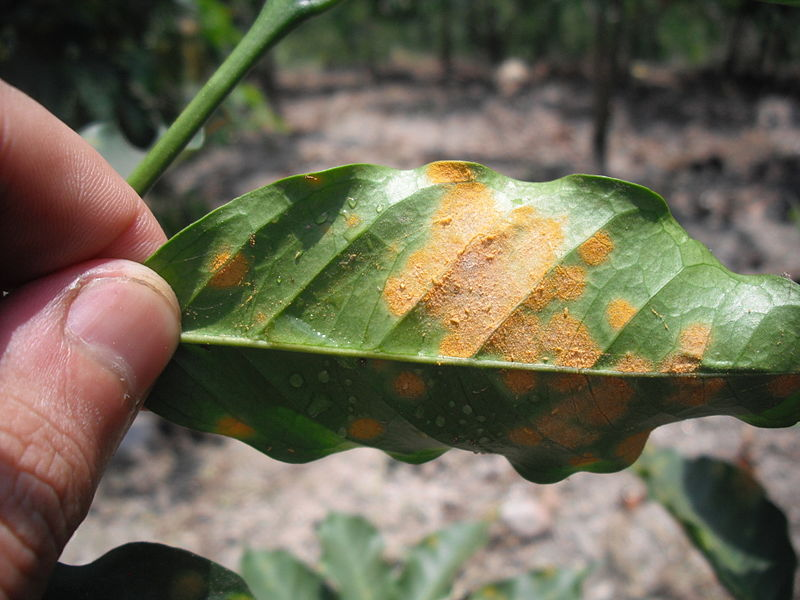
\includegraphics[width=0.8\linewidth]{./images/hemileia_vastatrix_coffee_leaf_rust} \end{center}

\textbf{Downy mildew of grapes}

Class: Oomycota
Order: Peronosporales

\emph{Plasmopara viticola}, also known as grape downy mildew, is considered to be the most devastating disease of grapevines in climates with relatively warm and humid summers. It was first observed in 1834 by Schweinitz on Vitis aestivalis in the southeastern United States. France was among the first of the European countries to gain experience in dealing with the pathogen. Within just a few years of the pathogen's introduction the French attempted to graft American root stock to their own vines in order to produce a more resistant strain of grape. Depending on the year, production of grapes in France has been estimated to have been reduced by as much as 50\%.

\begin{center}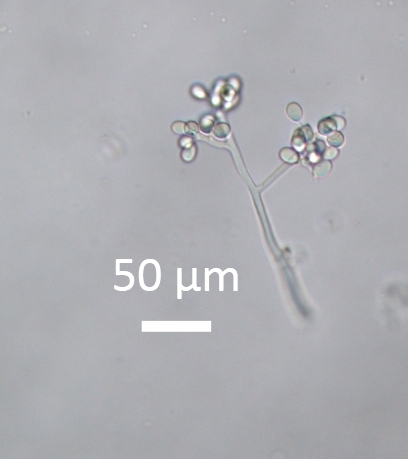
\includegraphics[width=0.8\linewidth]{./images/Plasmopara_vitticola} \end{center}

\textbf{Bengal famine of 1943}

The Bengal famine stroke Bengal province of British India during World war II. An estimated 2.1-3 million, out of a population of 60.3 million, died of starvation, malaria, or other diseases aggravated by malnutrition, population displacement and other causes. Affecting of winter rice with a severe outbreak of fungal brown spot disease ( \emph{Helminthosporium oryzae}) is considered to have a major role in the exacerbation of famine besides, political and other causes, cyclone particularly.

\hypertarget{disease-pests}{%
\section{Disease pests}\label{disease-pests}}

\hypertarget{rust}{%
\subsection{Rust}\label{rust}}

\textbf{Management}

Macrocyclic disease: \emph{Puccinia graminis} is a macrocyclic heteroecious fungus that causes wheat stem rust disease. The repeating stage in this fungus occurs on wheat and not the alternate host, barberry. The repeating stage allows the disease to persist in wheat even though the alternate host may be removed. Planting resistant crops is the ideal form of disease prevention, however, mutations can give rise to new strains of fungi that can overcome plant resistance. Although the disease cannot be stopped by removal of the alternate host, the life cycle is disrupted and the rate of mutation is decreased because of reduced genetic recombination. This allows resistance bred crops to remain effective for a longer period of time.

Demicyclic Disease: Because there is no repeating stage in the life cycle of demicyclic fungi, removal of the primary or the alternate host will disrupt the disease cycle. This method, however, is not highly effective in managing all demicyclic diseases. Cedar-apple rust disease, for example, can persist despite removal of one of the hosts since spores can be disseminated from long distances. The severity of Cedar-apple rust disease can be managed by removal of basidiospore producing galls from junipers or the application of protective fungicides to junipers.

Sulphur powder is known to stop spore germination. Fungicides such as Mancozeb and Triforine may help but may never eradicate the disease.

\textbf{Common rust fungi in agriculture}

\begin{itemize}
\tightlist
\item
  \emph{Hemileia vastatrix} (Coffee rust); Primary host is coffee plant; unknown alternate host. Heteroecious
\item
  \emph{Phakopsora meibomiae} and \emph{P. pachyrhizi} (Soybean rust); Primary host is soybean and various legumes. Unknown alternate host. Heteroecious
\item
  \emph{Puccinia coronata} (Crown Rust of Oats and Ryegrass); Oats are the primary host; Rhamnus spp. (Buckthorn) is alternate host. Heteroecious and macrocyclic
\item
  \emph{Puccinia graminis} (Stem rust of wheat and Kentucky bluegrass, or black rust of cereals); Primary hosts include: Kentucky bluegrass, barley, and wheat; Common barberry is the alternate host. Heteroecious and macrocyclic
\item
  \emph{Puccinia hemerocallidis} (Daylily rust); Daylily is primary host; Patrina sp is alternate host. Heteroecious and macrocyclic
\item
  \emph{Puccinia triticina} (Brown Wheat Rust) in grains
\item
  \emph{Puccinia sorghi} (Common Rust of Corn)
\item
  \emph{Puccinia striiformis} (Yellow Rust) of cereals
\item
  \emph{Uromyces appendiculatus} (Bean Rust) in common bean (Phaseolus vulgaris){[}16{]}
\item
  \emph{Puccinia melanocephala} (Brown Rust of Sugarcane)
\item
  \emph{Puccinia kuehnii} (Orange rust of Sugarcane)
\end{itemize}

\textbf{UG99}

It is a lineage of wheat stem rust ( \emph{Puccinia graminis f.~sp. tritici}), which is present in wheat fields in several countries in Africa and Middle east and is predicted to spread rapidly through these regions and possibly further afield, potentially causing a wheat production disaster that would affect food security worldwide. It can cause up to 100\% crop losses and is virulent against many resistance genes which have previously protected against stem rust.

\hypertarget{citrus-decline-in-nepal}{%
\subsection{Citrus decline in Nepal}\label{citrus-decline-in-nepal}}

Citrus greening disease or HLB was first reported from China in 1919 by Reinking while evaluating diseases of economic plants in southern China and used English term ``yellow shoot'' of citrus in the report. At that time it was believed that the HLB was caused by abiotic factors like Zn deficiency/toxicity and poor drainage system. By 1967, it became established that greening was graft and insect transmissible with conclusion caused by virus (Bove 2006). In 1967, mycoplasm like organisms (MLOs) were believed to be associated with plant diseases mostly with ``yellow'' symptoms resembling with greening symptoms. On close examination, these organisms were seen to have bacterial cell wall in addition to cytoplasmic membrane, suggesting that they were gram negative true bacteria (Garnier and Bove 1977). Thus, it was concluded that the HLB agent was gram negative bacterium -- \emph{Liberobacter asiaticus}.

Citrus decline was reported for the first time in Pokhara valley by Thrower (1968) in Nepal. Based on visual observation, Knorr et al (1970) suspected that the decline was caused by greening disease entered with the planting materials introduced to Horticulture Research Station, Pokhara from Saharanpur, India. About 55\% of citrus trees in Pokhara valley and 100\% in Horticulture Research Station were symptomatic to HLB in 1980s (Regmi 1982).

More recent PCR test showed that HLB is widespread in many citrus pockets of Kaski, Syanja, Tanahu, Lamjung and Dhading districts (Bove 2006 Regmi and Yadav 2007 Regmi et al 2010).

\textbf{Diagnosis of Citrus decline}

Visual symptoms are apparent on leaves and fruits. A tree infected with HLB in the field usually develops one or more yellow shoots with other parts of the tree healthy or symptomless. The affected leaves develop a pattern of yellow and green areas lacking clear limits between the colors, giving a ``blotchy mottle'' appearance. This is the most characteristic foliar symptom and the patterns are asymmetrical on the two halves of the leaf (Bove 2006). Leaves can also become thicker, with veins enlarged and corky in appearance. In later stages, Zn deficiency-like symptoms can be seen followed by leaf drop and twig dieback.

Currently, other methods besides visual diagnosis of Huanglongbang are molecular marker based test (quantative PCR), biological indexing, iodine test and spectroscopy. Based on severity of HLB symptoms and the ability to continue growth of the plants inoculation with \emph{Ca.} L. \emph{asiaticus} Folimonova et al (2009) grouped citrus genotypes into four categories as
i. sensitive: C. halimii, Nules clementine mandarin, Minneola tangelo, sweet oranges and grapefruit
ii. moderately tolerant: Sun Chu Sha mandarin, sour orange, volkamer lemon, C. macrophylla, wingle citrumelo, citron, Palestine sweet lime, acid lime, calamondin, and C. micrantha
iii. tolerant: Eureka lemon, Persian lime, Carrizo citrange, and Severinia buxifolia
iv. variable (some branch sensitive and some branch tolerant): pummelos, C. amblycarpa, cleopatra mandarin, C. indica, and meiwa kumquat.

\textbf{Citrus greening control}

\begin{itemize}
\item
  Inoculum reduction and vector control: Planting of certified clean planting materials, effective control of its vector psyllid populations and removal of infected trees that serve as an inoculums source for psyllid acquisition are the methods of choice. Biological control of the psyllid vector is only possible in locations that do not favour build-up of psyllid populations and is often compromised when hyper-parasites are present.
\item
  Chemical control: Combination of penicillin and streptomycin (PS) was effective in eliminating or supressing the bacterium.
\item
  Nutrition: Preliminary results of the research showed that HLB-infected trees are consistently deficient in Ca, Mg, Mn, Zn and B, and in an orchard. The main cause of visible HLB symptoms, yield reduction, and tree decline appears to be disruption of phloem tissue, which blocks the flow of photosynthate and nutrients from source to sink tissue. Hence plant growth enhancers, mainly that of root system should, to some extent, alleviate the symptoms of HLB.
\item
  Use of tolerant rootstocks: The citrus rootstock US-897 ( \emph{Citrus reticulata} Blanco x \emph{Poncirus trifoliata} L. Raf.) was observed to be tolerant to HLB in field plantings.
\item
  Guava intercropping: An observation in Vietnam in 2000, noted that the normal life of sole citrus plantings in Mekon region was 2 to 4 years, but those interplanted with white guava were surviving for up to 15 years (Gottwald et al 2010). Raising guava as an intercrop reduced psyllid population in citrus orchards.
\end{itemize}

\hypertarget{guava-wilt}{%
\subsection{Guava wilt}\label{guava-wilt}}

Causative agent: \emph{Fusarium oxysporium f.~psidi}, \emph{Rhizoctonia spp.}

Guava plants are attacked by wilt causing pathogen, which alone causes heavy losses in Nepalese guava trees. Yellowing and browning of leaves from the twigs tip. Leaves die off causing cracking in the twigs and trunk leading to the complete wilting and decline of entire tree. The incidence is more severe in alkaline soil and during winter season.

\textbf{Control measures}

\begin{itemize}
\tightlist
\item
  It is better to remove such trees as soon as the symptoms are identified to prevent the spread of disease.
\item
  Apply 15 gm of bavistin at the basin of each plant after pruning in March, June and September.
\item
  Liming of the pits.
\item
  Use of resistant root stock such as chinese guava and wilt resistant variety like Allahabad safeda, Banarasi, Nasik etc.
\end{itemize}

\hypertarget{fruit-rot-of-guava}{%
\subsection{Fruit rot of guava}\label{fruit-rot-of-guava}}

Causative agent: \emph{Phomopsis psidi}

This is a serious disease especially during rainy seasons. The symptoms are manifested as development of dark brown circular spots at the blossom end of the immature green fruits.

Control measures: Application of Zineb (0.2\%) or aureofungin (10 ppm) as monthly sprays during June to October can control the disease. Apply Kavach/Rovral (2g/ltr) and Carbendazim (1 g/ltr) during rainy season.

\hypertarget{fruit-canker}{%
\subsection{Fruit canker}\label{fruit-canker}}

Causative agent: \emph{Pestalotiopsis psidi}

Cankerous growth on fruit leading to cracking of fruits.

Control measures: Apply Dilhan 278 (2g), Cuman L (4 ml/ltr) and Rovral (2g/ltr) during rainy season.

\hypertarget{chirke-and-furket-of-cardamom}{%
\subsection{Chirke and furket of Cardamom}\label{chirke-and-furket-of-cardamom}}

\hypertarget{downy-mildew-of-cucumber}{%
\subsection{Downy mildew of cucumber}\label{downy-mildew-of-cucumber}}

\hypertarget{stemphyllium-blight-of-lentil}{%
\subsection{Stemphyllium blight of lentil}\label{stemphyllium-blight-of-lentil}}

\hypertarget{root-knot-nematode-of-tomato-brinjal-and-ladys-finger}{%
\subsection{Root knot nematode of Tomato, Brinjal and Lady's finger}\label{root-knot-nematode-of-tomato-brinjal-and-ladys-finger}}

\hypertarget{pesticides}{%
\section{Pesticides}\label{pesticides}}

\hypertarget{history}{%
\subsection{History}\label{history}}

\begin{itemize}
\tightlist
\item
  The oldest available record is Homer's mention (about 1000 BC) that Odysseus burned sulfur to purge the hall and the house and the court.
\item
  In 1669, the earliest known record of arsenic as an insecticide in the western world mentioned its use with honey as an ant bait.
\item
  Use of tobacco as contact insecticide was mentioned later in the same century.
\item
  Copper compounds were known since 1807 to have fungicidal value, and the Bordeaux mixture (hydrated lime and copper sulfate) was first used in France in 1883.
\item
  Hydrocyanic acid, known to the egyptians and the Romans as a poison, was used as a fumigant in 1877 to kill museum pests in insect collections.
\item
  Carbon disulfide has been used as an insect fumigant since 1854.
\item
  Mercury chloride was extensively used as fungicide since 1891, and was slowly replaced by its organic forms such as phenylmercury (1915), alkylxyalkylmercury (1920s).
\item
  First synthetic organic insecticides that appeared for public use was probably dinitro compounds and thiocyanates (in early 1930s)
\item
  These led to proliferation of new synthetic pesticides including DDT, organophosphates and pyrethroids.
\item
  Paul Muller (awarded nobel prize in Medicine for his discoveries) in 1939 found dichlorodiphenyltrichloroethane (DDT) acted as a contact poison on flies, mosquitores, and other insects. In 1945, monsanto begins manufacturing 2,4-D.
\item
  In 1949, case of human exposure to dioxin causing severe skin lesions was first documented.
\item
  Organic sulfur fungicides such as captan, maneb and others were introduced in late 1950's, however some are known to have toxicological problems.
\item
  In 1972 EPA banned DDT.
\item
  In developing countries where the risk of contracting malaria is extremely high, DDT is permitted as a tool for mosquito population control. The benefit of suppressing the malaria-transmitting mosquitoes outweighs the risk of DDT exposure.
\item
  Production of DDT in the USA peaked in the early 1960's and gradually declined.
\item
  In 1962 Rachel Carson published the book Silent Spring, an impassioned denouncement of the consequences of chemical contamination of the environment, with particular emphasis on the bioaccumulation of DDT and its effects on bird reproduction.
\item
  Pyrethroids derive from molecules originally isolated from pyrethrum flowers which were used by Gaucasian tribes and in Persia since the early 1800's to control body lice. The flower extracts contain six closely related insecticidal esters, collectively referred to as the pyrethrins, whose main structures were elucidiated between 1910 and 1924.
\item
  Some of the most commonly used pyrethroid insecticides, such as permethrin, cypermethrin, decamethrin and fenvalerate, were synthesized in the 1970s.
\end{itemize}

\begin{table}

\caption{\label{tab:unnamed-chunk-8}Some toxicologically-related events involving pesticides}
\centering
\begin{tabular}[t]{ll}
\toprule
Year & Event\\
\midrule
1930s & 'Ginger jake' paralysis in the US caused by cresyl phosphates\\
1962 & Silent spring by Rachel Carson published\\
1970-73 & Restriction in the use of DDT in Sweden and US for its ecological effects\\
1971-72 & Outbreak of poisoning in Iraq due to alkylmercury fungicides\\
1976 & Poisoning of spraymen in Pakistan by malathion due to its potentiation by impurities\\
\addlinespace
1977 & Restriction on the use of dibromochloropropane for its toxicity on the male reproductive system\\
1984 & Accidents in Bhopal during the manufacture of carbaryl\\
1986 & Over 1000 tons of pesticides are spilled in the Rhine river\\
\bottomrule
\end{tabular}
\end{table}

\hypertarget{brief-history-of-ddt}{%
\subsection{Brief history of DDT}\label{brief-history-of-ddt}}

DDT (dichloro-diphenyl-trichloroethane) was developed as the first of the modern synthetic insecticides in the 1940s. It was intially used with great effect to combat malaria, typhus, and the other insect-borne human diseases among both military and civilian populations adn for insect control in crop and livestock production, institutions, homes and gardens. DDT's quick success as a pesticide and broad use in the US and other countries led to the develpment of resistance by many insect pest species. The US Department of Agriculture, the federal agency responsible for regulating pesticides before the formation of the US Environmental Protection Agency in 1970, began regulatory actions in the late 1950s and 1960s to prohibit many of DDT uses because of mounting evidence of the pesticide's declining benefits and environmental and toxicological effects. Rachel Carson's book Silent Spring in 1962 stimulated widespread public concern over the dangers of improper pesticide use and the need for better pesticide controls. DDT was firstly banned in 1972 by many European nations.

\hypertarget{stockholm-convention}{%
\subsection{Stockholm convention}\label{stockholm-convention}}

The stockholm convention was brought about as a global treaty to protect human health and the environment from persistent organic pollutants (POPs). The convention seeks the elimination or restriction of production and use of all intentionally produced POPs (i.e.~industrial chemical pesticides), and the continuing minimization and, where feasible, ultimate elimination of releases of unintentionally produced POPs, such as dioxins and furans. Stockpiles must be managed and disposed off in a safe, efficient, environmentally sound manner. The convention was finalized at the 5th Intergovernmental Negotiating Committee (INC) Meeting in Johannesburg in December, 2000. The signing and adoption of the Stolkholm Convention took place in Stolkholm on 23 May 2001 with entry into force following on 17th May 2004 after the fiftieth ratification. Currently, 176 countries are parties to the Convention.

\begin{table}

\caption{\label{tab:banned-pesticides}List of pesticides banned in Nepal.}
\centering
\begin{tabular}[t]{rlrl}
\toprule
Sn & Pesticide & Year banned & Remark\\
\midrule
\rowcolor{gray!6}  1 & Chlordane & 2001 & \\
2 & DDT & 2001 & \\
\rowcolor{gray!6}  3 & Dieldrin & 2001 & \\
4 & Endrin & 2001 & \\
\rowcolor{gray!6}  5 & Aldrin & 2001 & \\
\addlinespace
6 & Heptachlor & 2001 & \\
\rowcolor{gray!6}  7 & Mirex & 2001 & \\
8 & Toxaphene & 2001 & \\
\rowcolor{gray!6}  9 & BHC & 2001 & \\
10 & Lindane & 2001 & \\
\addlinespace
\rowcolor{gray!6}  11 & Phosphamidon & 2001 & \\
12 & Organo mercury fungicides & 2001 & \\
\rowcolor{gray!6}  13 & Methyl parathion & 2007 & \\
14 & Monocrotophos & 2007 & \\
\rowcolor{gray!6}  15 & Endosulfan & 2014 & \\
\addlinespace
16 & Phorate & 2015 & Use and distribution allowed untill 2077-09-16\\
\rowcolor{gray!6}  17 & Benomyl & 2018 & Use and distribution allowed untill 2077-09-16\\
18 & Carbofuran & 2018 & Use and distribution allowed untill 2077-09-16\\
\rowcolor{gray!6}  19 & Triozophos & 2018 & Use and distribution allowed untill 2077-09-16\\
20 & Dichlorovus & 2018 & Use and distribution allowed untill 2077-09-16\\
\addlinespace
\rowcolor{gray!6}  21 & Carbaryl & 2018 & Use and distribution allowed untill 2077-09-16\\
22 & Carbosulfan & 2019 & Use and distribution allowed untill 2078-04-19\\
\rowcolor{gray!6}  23 & Dicofol & 2019 & Use and distribution allowed untill 2078-04-19\\
24 & Aluminium Phosphide & 2019 & Use and distribution allowed untill 2078-04-19\\
\bottomrule
\end{tabular}
\end{table}

\hypertarget{additional-information}{%
\subsection{Additional information}\label{additional-information}}

Annotations used in describing formulations:
- GR: Granule
- CG: Encapsulated granule
- SP: Soluble powder
- DP: Dusting powder
- WP: Wettable powder

\hypertarget{chemical-fungicides}{%
\subsection{Chemical fungicides}\label{chemical-fungicides}}

\begin{itemize}
\tightlist
\item
  A popular fungicide, generally used for seed treatment, called Carbendazim is available in commercial formualtion as KI-BESTIN (Carbendazim 50\% WP).

  \begin{itemize}
  \tightlist
  \item
    The commercial seed treatment fungicide is composed of:

    \begin{itemize}
    \tightlist
    \item
      51\% Carbendazim 98\% (at minimum) a.i.
    \item
      2\% Surface acting agent
    \item
      2\% Dispersing agent
    \item
      2\% Sticking agent (Glue powder)
    \item
      43\% Inert carrier (China clay)
    \end{itemize}
  \item
    In case of carbendazim poisoning medical charcoal preparation 6-10 times is recommended.
  \item
    It has green colored warning level.
  \item
    It is manufactured by Kisan Agro Chemicals, Parsa, Birgunj, Nepal.
  \item
    KI-BESTIN is a broad spectrum systemic fungicide useful as both spray and wetted powder form.
  \end{itemize}
\end{itemize}

\hypertarget{biopesticides}{%
\subsection{Biopesticides}\label{biopesticides}}

\begin{itemize}
\tightlist
\item
  \emph{Trichoderma viridae} (Nisarga, Nicoderma, Bio-Powder-F)

  \begin{itemize}
  \tightlist
  \item
    Available as 1\% or 1.15\% AI WP formulation.
  \item
    Effectiveness: Stem rot, Root rot, Sett rot, Damping off, Ganoderma etc. Against \emph{Fusarium}, \emph{Sclerotium}, \emph{Phytopthora} and \emph{Ganoderma}.
  \item
    Utility crops: Potato, tomato, sweet pepper, garlic, cauliflower, onion, tea, coffee and pulses.
  \item
    Dosage: Spray 5 gm Nisarga per liter of water solution. While applying in soil, 500 gm Nisarga is mixed with 2.5 kg of mature FYM or compost. This suffices for 1 ropani of land.
  \end{itemize}
\item
  \emph{Pseudomonas}

  \begin{itemize}
  \tightlist
  \item
    Active ingredient: \emph{Pseudomonas fluorescence}
  \item
    Effectiveness: Onion smut, Paddy blast, Bacterial wilt of pepper and Dieback of tomato.
  \item
    Useful against soil borne, seed borne and air borne pathogens.
  \item
    Secondary metabolites, i.e.~Auxin, Gibberelic acid and Cytokinins promote plant health.
  \item
    Dosage: Spray 5 g of Pseudomonas commercial formula in 1 liter of water. While applying in soil, 500 gm Nisarga is mixed with 2.5 kg of mature FYM or compost. This suffices for 1 ropani of land.
  \end{itemize}
\item
  \emph{Beauveria bassiana} (BABA, BIO-Powder)

  \begin{itemize}
  \tightlist
  \item
    Active ingredient 1.15\%
  \item
    Available in WP formulation
  \end{itemize}
\item
  \emph{Verticillium lecani} (Mealikil(TM))

  \begin{itemize}
  \tightlist
  \item
    Available as 1.15\% WP formulation
  \item
    Verticillium fungicide is effective against sucking insects and nematodes.
  \item
    In a ropani of land, use 500 gm of verticillium preparation with 2.5 kg of FYM/compost.
  \end{itemize}
\item
  Azadirachtin (Nimbicidine, Multineem, Multinemor, Niconeem, Neemate-10, Ozoneem Trishul)

  \begin{itemize}
  \tightlist
  \item
    Effectiveness: Against phytophagous insects for deterrence. It inhibits oviposition and is ovicidal (kills larvae if hatched)
  \item
    Most effective against sap sucking type insects (Aphid, mealy bug, white fly, thrips, etc.) and chewing type insects (Stem and fruit borer larvae)
  \item
    Has contact and systemic property
  \item
    Dosage: 2-5 ml liquid in 1 ltr of water is sprayed in 12 days interval, 2-3 times.
  \item
    Composition: 0.03\%, 0.15\%, 1\%, etc.
  \end{itemize}
\item
  \emph{Metarhizium anisopliae} (Pacer (TM))

  \begin{itemize}
  \tightlist
  \item
    Available as 1.15\% WP formulation
  \end{itemize}
\item
  Nuclear polyhedrosis virus (NPV)
\item
  Granulosis virus (GVs)
\end{itemize}

\hypertarget{rodenticides}{%
\subsection{Rodenticides}\label{rodenticides}}

\begin{itemize}
\tightlist
\item
  Bromadiolone (Ratonil, Krazy ratmaar, Roban) available as 0.005-0.25\% RB, WP and CB formulation.
\item
  Zinc phosphide (All commando, Commando, K-rat, Ratal, Ratfre, Ratil, Ratox) available as 80\% WW formulation.
\end{itemize}

\hypertarget{waiting-periods-of-some-pesticides}{%
\subsection{Waiting periods of some pesticides}\label{waiting-periods-of-some-pesticides}}

\begin{longtable}[t]{>{\raggedleft\arraybackslash}p{4em}>{\raggedleft\arraybackslash}p{6em}>{\raggedleft\arraybackslash}p{6em}>{\raggedleft\arraybackslash}p{20em}}
\caption{\label{tab:unnamed-chunk-9}Waiting period of some commonly used pesticides}\\
\toprule
Sn & Waiting period (days) & Group & Common name\\
\midrule
\rowcolor{gray!6}  1 & 1 & Bactericide & Streptomycin sulphate + Tetracycline hydrochloride\\
2 & 3 & Botanical & Azadirachtin, Metarhizium anisopliae, Pseudomonas flurescens\\
\rowcolor{gray!6}  3 & 3-5 & Insecticide & Dichlorovos\\
4 & 4 & Insecticide & Beta-cyfluthrin\\
\rowcolor{gray!6}  5 & 5 & Insecticide & Novaluron, Buprofezin\\
\addlinespace
6 & 5 & Miticide & Fenpyroximate\\
\rowcolor{gray!6}  7 & 6 & Insecticide & Bifenthrin\\
8 & 6 & Miticide & Dicofol\\
\rowcolor{gray!6}  9 & 6 & Fungicide & Metiram\\
10 & 3-7 & Insecticide & Fenpyroximate\\
\addlinespace
\rowcolor{gray!6}  11 & 7 & Insecticide & Cyfluthrin, Alphamethrin, Cypermethrin, Cyromazine, Deltamethrin, Diflubenzuron, Fenvalarate, Thiodicarb\\
12 & 7 & Botanical & Beuveria bassiana, Trichoderma viride, Verticillium lecani\\
\rowcolor{gray!6}  13 & 7 & Weedicide & 2-4 D NA salt, Pyrazosulfuron ethyl\\
14 & 10 & Insecticide & Emamectin benzoate\\
\rowcolor{gray!6}  15 & 10 & Fungicide & Zineb\\
\addlinespace
16 & 14 & Insecticide & Abamectin, Alphacypermethrin, Carbofuran, Ethion, Lambdacyhalothrin, Lufenuron, Malathion, Profenofos, Triazophos\\
\rowcolor{gray!6}  17 & 14 & Miticide & Propargite\\
18 & 14 & Fungicide & Carbendazim, Chlorothalonil, Copper hydrochloride, Copper hydroxide, Cymoxanil, Dimethomorph, Iprobenfos, Kresoxim, Methyl sulphur, Thiophanate methyl\\
\rowcolor{gray!6}  19 & 15 & Insecticide & Acephate, Acetamiprid, Dimethoate\\
20 & 15 & Weedicide & Oxyfluorfen\\
\bottomrule
\end{longtable}

\hypertarget{pathogenic-nematodes}{%
\section{Pathogenic Nematodes}\label{pathogenic-nematodes}}

\begin{itemize}
\item
  Nematode is derived from the Greek words, ``Nema'' = thread/fibre, ``toda'' = worm.
\item
  In germany, there is a separate University of Nematology.
\item
  Nematodes can be defined as unsegmented, bilaterally symmetrical, tryploblastic, pseudocoelomate, invertebrate, and thread like worms.
\item
  So far 50000 nematode species are recorded worldwide. 10000 are found in fresh water and soil. 300 species are known to be plant parasites.
\item
  Molya disease ( \emph{Heterodera avenae}) causes 6-7 crore/year loss in Rajasthan and ear cockle ( \emph{Anguina tritici}) causes 8 crore loss in India.
\item
  \emph{Radopholus similis} was found associated with citrus decline in Florida, USA.
\item
  In India, \emph{Tylenchulus semipenetrans} was associated with citrus decline.
\item
  Plant parasitic nematodes are triploblastic, bilaterally symmetrical, unsegmented, pseudocelomate and vermiform animals.
\item
  The body of the nematode may be elongated, spindle shaped, fusiform tapering towards the end but the cross section is always circular.
\item
  Smallest nematode is 10mm long ( \emph{Paralongidorus}).
\item
  Female nematodes are more virulent and agressive than male in attacking and parasitizing the plants.
\item
  Plant parasitic nematode possess spear or stylet.
\item
  Nematodes are known to transmit viruses:

  \begin{itemize}
  \tightlist
  \item
    Two single stranded RNA virus genera, Nepovirus (NEPO) and Tobravirus (TOBRA).
  \item
    11 species of Xiphinema transmit 13 NEPO virus (Grapevine fan leaf virus)
  \item
    11 species of Longidorus transmit 10 NEPO virus
  \item
    14 species of Trichodorus transmit various strains of TOBRA virus: tobacco rattle and pea early browning
  \end{itemize}
\end{itemize}

\textbf{Insect transmitted viruses}

\begin{table}

\caption{\label{tab:insect-transmissed-viruses}Insect mediated virus transmission}
\centering
\begin{tabular}[t]{ll}
\toprule
Virus & Nematode\\
\midrule
\rowcolor{gray!6}  Rice dwarf virus & Nephotettix cincticeps\\
Rice tungro virus & Nephotettix impicticeps\\
\rowcolor{gray!6}  Rice grassy stunt virus & Nilaparvata lugens\\
Tomato spotted wilt virus & Thrips tabaci, Frankliniella spp.\\
\rowcolor{gray!6}  Tomato yellow leaf curl virus & Bemisia tabaci\\
\addlinespace
Tomato yellow mosaic virus & Bemisia tabaci\\
\rowcolor{gray!6}  Soybean yellow mosaic & Bemisia tabaci\\
Grapevine virus A & Pseudococcus longispinus (Mealybugs)\\
\rowcolor{gray!6}  Cowpea mosaic virus & Epilachna varivestis\\
Potato virus X virus & Melanoplus differentialis (Grasshopper)\\
\addlinespace
\rowcolor{gray!6}  Tobacco mosaic virus & Liriomyza langei (Leafminer); Mechanical transmission\\
Onion mosaic virus & Eriophyses tulipae (Mites)\\
\rowcolor{gray!6}  Soybean mosaic virus & Aphids\\
Potato leaf roll virus & Myzus persicae\\
\bottomrule
\end{tabular}
\end{table}

\hypertarget{crop-diseases}{%
\section{Crop diseases}\label{crop-diseases}}

\hypertarget{ergot-wheat-barley-oats-rye-triticale}{%
\subsection{Ergot (Wheat, barley, oats, rye, triticale)}\label{ergot-wheat-barley-oats-rye-triticale}}

Hosts:
All grasses, particularly, blackgrass ( \emph{Alopecurus myosuroides})

Symptoms:

\begin{itemize}
\tightlist
\item
  Causal fungus only attacks ears of flowering, replacing the grain in a few spikelets by a hard, purple black sclerotium, known as ergot.
\item
  Such ergots can be very large, upto 2 cm in length, and very obvious in the standing crop in contaminated grain samples.
\end{itemize}

Life cycle:

\begin{itemize}
\tightlist
\item
  Ergot is not truely a seed borne disease, however it can be spread by ergots in contaminated seeds.
\item
  At or near harvest, ergots fall to the ground where they remain untill the following summer, when they germinate to produce club-shaped spore bearing structure (stroma). These ascospores are spread by the wind to nearly open flowers of grasses/cereals. The spores germinate in flower, infecting the ovaries. This infection leads to the production of secondary spores (condia) encased in sticky secretion commonly referred to as honeydew. This attracts insects which carry the spores to other flowers, where further infection can occur.
\item
  Wheat and other cereals are less severely affected than rye although, occassionally more open-flowerd wheat variety can be badly affected.
\item
  Disease is favored by cool, wet conditions during flowering which facilitate spore production and prolong the flowering period, making infection more likely.
\end{itemize}

Importance:

\begin{itemize}
\tightlist
\item
  Very little direct effect on yield.
\item
  Affects stocks which when fed to flour made with cereals with large amount of toxic alkaloid containing ergot, possess health risks.
\end{itemize}

\hypertarget{fusarium}{%
\subsection{Fusarium}\label{fusarium}}

Fusariusm head blight/ear blight, foot rot, seedling blight
Pathogen: \emph{Fusarium spp.} and \emph{Microdochium nivale}
Hosts: Wheat, barley, oats, rye triticale and grasses.

Symptoms:

\begin{itemize}
\tightlist
\item
  Form a complex of diseases on seeds, seedlings and adult plants.
\item
  \emph{Microdochium nivale} (formerly known as \emph{Fusarium nivale}) is seed-borne pathogen and causes seedling blight resulting in seedling death and thinning of plant stand.
\item
  \emph{M. spp} (other than \emph{M. nivale}) cause a range of symptoms including brown lesions on stem bases, often restricted to outer leaf sheath.
\item
  \emph{Fusarium lesions} often begin in the leaf sheath at the stem base where crown roots split the leaf sheath when emerging.
\item
  This infection can spread up the leaf sheath causing long dark brown streaks at the stem base. The other symptom in cooler regions is brown staining of lower nodes.
\item
  In older plants, fusarium infection can produce a true foot rot, where the stem base becomes brown and rotten, resulting in lodging and white heads.
\item
  Symptoms are prevalent in very dry seasons as well.
\item
  Ear blight causing fungus: \emph{F culmorum} and \emph{F graminearum} are common. Other are, \emph{F avenaceum}, \emph{F poae} and \emph{F langsethiae}.
\item
  Infection frequently results in the whole or part of the ear becoming bleached.
\item
  Symptoms seen when ears become infected during the early flowering stages, later infection may result in infection of grain but without obvious bleaching of the ears.
\item
  Important due to its mycotoxin that gets accumulated in grains.
\end{itemize}

Life cycle:

\begin{itemize}
\tightlist
\item
  Most important source is seed but fungus survives on debris in soil also.
\item
  Spores are splashed in canopy causing ear blights and seed borne infection, in wet seasons, especially during flowering and grain formation.
\item
  Most fusarium species have competative saprophytic abilities which allow them to colonize debris and stubble in soil.
\end{itemize}

Importance:

\begin{itemize}
\tightlist
\item
  When wet season coincides with flowering high levels of ear blight can occur.
\item
  Due to seed borne nature of pathogen, seed treatment plays role in preventing seedling loss in wheat.
\end{itemize}

\hypertarget{major-diseases-of-rice}{%
\subsection{Major diseases of rice}\label{major-diseases-of-rice}}

\begin{enumerate}
\def\labelenumi{\arabic{enumi}.}
\tightlist
\item
  Blast
\end{enumerate}

\begin{itemize}
\tightlist
\item
  Bavistin, Dorosal 2-3 g per kg seed treatment
\item
  Tricyclazole 75\% WP 0.75 g per ltr spray at 15 days interval
\item
  Kasugamycin 3\% SL 1.5 ml per ltr at 15 days interval
\end{itemize}

\begin{enumerate}
\def\labelenumi{\arabic{enumi}.}
\setcounter{enumi}{1}
\tightlist
\item
  Bacterial leaf blight
\end{enumerate}

\begin{itemize}
\tightlist
\item
  Use Agromycin-100 0.25 g per ltr for seed soaking for 30 minutes
\end{itemize}

\begin{enumerate}
\def\labelenumi{\arabic{enumi}.}
\setcounter{enumi}{2}
\tightlist
\item
  Brown leaf spot disease
\end{enumerate}

\begin{itemize}
\tightlist
\item
  Bavistin, Dorosal
\item
  Apply Mancozeb 75\% WP (Dithane M-45) 3 g per ltr water, Propineb 70\% WP 3 g per ltr water at 15 days interval for 3 times.
\end{itemize}

\begin{enumerate}
\def\labelenumi{\arabic{enumi}.}
\setcounter{enumi}{3}
\tightlist
\item
  Foot rot
\end{enumerate}

\begin{itemize}
\tightlist
\item
  Carbendazim 50\% WP seed treatment
\end{itemize}

\begin{enumerate}
\def\labelenumi{\arabic{enumi}.}
\setcounter{enumi}{4}
\tightlist
\item
  Sheath blight
\end{enumerate}

\begin{itemize}
\tightlist
\item
  Maintain spacing
\item
  Validamycin 3\% L 3 g per ltr water; Pencycuron 22.9 SC 1.5 ml per ltr; Carbendazim 70\% WP 1.5 g per ltr spray at 10-12 days interval for two times.
\end{itemize}

\begin{enumerate}
\def\labelenumi{\arabic{enumi}.}
\setcounter{enumi}{5}
\tightlist
\item
  Khaira disease
\end{enumerate}

\begin{itemize}
\tightlist
\item
  20 g \(\mathrm{ZnSO_4}\) + 12\% \(\mathrm{CaCO_3}\) in 50 ltr water per ropani at 10 days interval for 2 times.
\end{itemize}

\hypertarget{major-diseases-of-wheat}{%
\subsection{Major diseases of Wheat}\label{major-diseases-of-wheat}}

\begin{enumerate}
\def\labelenumi{\arabic{enumi}.}
\tightlist
\item
  Leaf blight
\end{enumerate}

\begin{itemize}
\tightlist
\item
  Small brown dots on leaves
\item
  Later on the dots coalesce to cause wilting or blighted appearance
\item
  Use Vitavex-200 2 gm per kg seed as presowing treatment
\item
  Increase potassium fertilizer dosage
\end{itemize}

\begin{enumerate}
\def\labelenumi{\arabic{enumi}.}
\setcounter{enumi}{1}
\tightlist
\item
  Brown rust
\end{enumerate}

\begin{itemize}
\tightlist
\item
  Orange color spots on upper surface of leaves.
\item
  Spots do not coalesce or merge
\item
  Mancozeb (Dithane M-45 45 WP) 1.5-2 kg in 750 ltr water spray at interval of 15 days for 2-3 times.
\end{itemize}

\begin{enumerate}
\def\labelenumi{\arabic{enumi}.}
\setcounter{enumi}{2}
\tightlist
\item
  Yellow rust
\end{enumerate}

\begin{itemize}
\tightlist
\item
  Yelow colored spots, elongated and jointed to form stripes
\item
  Cultivation of resistant varieties: WK-1204, Pasang Lhamu.
\end{itemize}

\begin{enumerate}
\def\labelenumi{\arabic{enumi}.}
\setcounter{enumi}{3}
\tightlist
\item
  Loose smut
\end{enumerate}

\begin{itemize}
\tightlist
\item
  Instead of grains black mass of fungal hyphae fills the panicle.
\item
  Use of healhty seeds, Vitavex-200 2 g per kg seed treatment
\item
  Bury the sick panicles in initial stage of disease appearance.
\item
  Annapurna variety is relatively tolerant to disease.
\end{itemize}

\begin{enumerate}
\def\labelenumi{\arabic{enumi}.}
\setcounter{enumi}{4}
\tightlist
\item
  Stinking smut/hill smut
\end{enumerate}

\begin{itemize}
\tightlist
\item
  Diseased grains are rounded, black colored spores filled
\item
  Spores only released after grain is crushed
\item
  Smell of fish
\item
  Crop rotaion for 2-3 years, Vitavex-200 2 g per kg seed treatment.
\end{itemize}

\begin{enumerate}
\def\labelenumi{\arabic{enumi}.}
\setcounter{enumi}{5}
\tightlist
\item
  Wheat blast
\end{enumerate}

\begin{itemize}
\tightlist
\item
  Wheat blast caused by \emph{Magnaporthe oryzae} (synonym \emph{Pyricularia oryzae}) pathotype Triticum. was first discovered in Brazil in 1985 and limited to South America until 2016.
\item
  Appeared in Bangladesh for the first time in february 2016.
\item
  Spread to several south-western and southern districts.
\item
  Covering 15\% of the total wheat area in Bangladesh.
\item
  About 15,000 ha was affected.
\item
  Emerged as a serious threat to the country's aggregate wheat production.
\item
  Initial symptoms appeared in mid February and worsened within 2 weeks.
\item
  Infected spikes were partially or wholly beached above the infection point on the rachis.
\item
  Infected samples were collected and examined at Wheat Research Centre, BARI, Dinajpur.
\item
  The identification is done based on typical:

  \begin{itemize}
  \tightlist
  \item
    Symptoms reported in South America
  \item
    Fungal growth on infected rachis in moist blotters
  \item
    Pyriform 2-septate conidia of P. oryzae.
  \end{itemize}
\item
  Blast infected grains are smaller in size.
\end{itemize}

\textbf{Disease epidemiology}

\begin{itemize}
\tightlist
\item
  The disease is seed-borne/transmitted
\item
  Disease develops in patches then spreads to whole plot by wind and or rain splash.
\item
  Heads are severely infected, while the canopy remains green.
\item
  \ldots{}
\end{itemize}

\hypertarget{major-diseases-of-jackfruit}{%
\subsection{Major diseases of jackfruit}\label{major-diseases-of-jackfruit}}

\begin{enumerate}
\def\labelenumi{\arabic{enumi}.}
\tightlist
\item
  Pink disease ( \emph{Botryobasidium salmonicolor})
\end{enumerate}

\hypertarget{entomology}{%
\chapter{Entomology}\label{entomology}}

\hypertarget{pesticide-toxicity}{%
\section{Pesticide toxicity}\label{pesticide-toxicity}}

\begin{itemize}
\item
  A pesticide is any substance used to control pests. Pests may be target insects, vegetation, fungi, etc. Most control the pests by poisoning them. Unfortunately, pesticides can be poisonous to humans as well.
\item
  Toxicity: The toxicity of a substance is its capacity to cause injury to a living system. A living system can be things such as a human body, parts of the body (lungs or respiratory system), a pond, a forest and those creatures that live in there. Toxicity represents the kind and extent of damange that can be done by chemical. In other words, if you know the toxicity of a pesticide, you know how poisonous it is.
\item
  Dose-time relationship of pesticide toxicity

  \begin{itemize}
  \tightlist
  \item
    Dose is the quantity of a substance that a surface, plant or animal is exposed to.
  \item
    Time means how often the exposure occurs.
  \item
    This relationship gives rise to two types of toxicity.
  \end{itemize}

  \begin{enumerate}
  \def\labelenumi{\arabic{enumi}.}
  \tightlist
  \item
    Acute toxicity: This refers to how poisonous a pesticide is to a human, animal or plant after a single-term exposure. It generally implies the effect that occurs within 24 hours of exposure.
  \item
    Chronic toxicity: This refers to delayed poisonous effects from exposure to substance.
  \end{enumerate}
\item
  Routes of entry:

  \begin{enumerate}
  \def\labelenumi{\arabic{enumi}.}
  \tightlist
  \item
    Local: local effect refers to those that take place at the site of contact with material. e.g.~skin irritation/inflammation on th hand in response to hand contact, irritation of mucous membrane lining the lungs due to inhalation of toxic fumes.
  \item
    Systemic: Effect that occur away from the original point of contact. These pesticides are distributed throughout the body once they enter. They function by blocking or stimulating a chemical signal, generally that of the nervous system (Cholinesterase).
  \end{enumerate}
\item
  Pesticides may have following actions:
\item
  Additive, antagonistic or synergistic
\item
  Immediate or delayed
\item
  Reversible or irreversible action
\item
  Exposure may result in following effects:

  \begin{itemize}
  \tightlist
  \item
    Reproductive effects
  \item
    Teratogenic effects: Effect on unborn offspring, such a birth defects.
  \item
    Carcinogenic effects: Cancer in living animal tissues.
  \item
    Oncogenic effects: Tumor forming effect (not necessarliy cancerous)
  \item
    Mutagenic effects: Permanent effect on genetic material that can be inherited
  \item
    Neurotoxicity: Poisoning of nervous system, including the brains.
  \item
    Immunosupression
  \end{itemize}
\end{itemize}

Acute toxicity measures

To figure out how acutely toxic a pesticide is, scientists give laboratory animals short-exposure to does of pesticide being tested. Experimental doses are given orally, as well as put on eyes, skin, and in the air that test animals breathe. These animals are then carefully observed for the changes.

\textbf{LD50}

Amount of a pesticide that has killed half of the animals in a laboratory test. LD50 values are effective for both oral and dermal routes of exposure. But they do not tell us about how the chemical acts, nor about how sensitive different organs within an animal or human might be. LD50 for different chemicals can be compared if the same test animial was used. The LD50 values are measured in unit of weight called mg per kg (or interchangeably, parts per million).

\textbf{LC50}

This measure of toxicity gives the acute inhalation toxicity.

Chronic toxicity measures

There is no standard measure like LD50 for chronic toxicity studies. Often the length of the experiment is in days, months or years and the amount of each dose is stated. For e.g., a study of chronic oral toxicity might look like, ``8 mg of pesticide to rats daily for two years. No symptoms of poisoning appeared.''

\begin{itemize}
\tightlist
\item
  Two classes of pesticides, organophosphates and carbamates can slowly poison by attacking an essential body chemical called ``cholinesterase''. The chronic exposure to Organophosphate pesticides can be measured by monitoring changes in blood cholinesterase levels. In humans, decrease in cholinesterase levels are sure sign that exposure to these types of pesticides should be avoided untill the level is measured as being normal again.
\end{itemize}

Categories of pesticide toxicity

\begin{table}

\caption{\label{tab:pesticide-hazard-category}Categories of pesticide toxicity}
\centering
\begin{tabular}[t]{lllll}
\toprule
Toxicity class & Toxicity label & Oral LD50 (mg/kg) & Dermal LD50 (mg/kg) & Inhalation LC50 (mg/L)\\
\midrule
Highly toxic & Danger & 0-50 & 0-200 & 0-0.2\\
Moderately toxic & Warning! & 50-500 & 200-2000 & 0.2-2\\
Slightly toxic & Caution!! & 500-5000 & 2000-20000 & 2-20\\
Relatively non-toxic & Caution!! & >5000 & >20000 & >20\\
\bottomrule
\end{tabular}
\end{table}

Status of pesticide use in Nepal

\begin{itemize}
\tightlist
\item
  Initially, DDT was imported in 1952 AD for control of Maleria.
\item
  For the same purpose, DDT was reimported in 1955 AD
\item
  For use in crops, DDT was imported in 1956 AD.
\item
  According to Thapa, 2003, average pesticide use in Nepal is 142 gm/ha.
\item
  In general, cropwise analysis of pesticide use signals alarming levels of residues, hence their current state of use being haphazard.

  \begin{itemize}
  \tightlist
  \item
    Tea: 2100 gm/ha
  \item
    Cotton: 2560 gm/ha
  \item
    Vegetables: 1400 gm/ha
  \end{itemize}
\item
  On environmental perspective, pesticides are of following types, based on bio-degradation:

  \begin{enumerate}
  \def\labelenumi{\arabic{enumi}.}
  \tightlist
  \item
    Environmentally degradable/non-persistent:
  \end{enumerate}

  \begin{itemize}
  \tightlist
  \item
    Dimethoate (Nuger, Roger, Dimet)
  \item
    Dichlorovos (Dum, Vapon)
  \item
    Fenitrothion (Folithion)
  \item
    Malathion
  \end{itemize}

  \begin{enumerate}
  \def\labelenumi{\arabic{enumi}.}
  \setcounter{enumi}{1}
  \tightlist
  \item
    Environmentally non-degradable/persistent:
  \end{enumerate}

  \begin{itemize}
  \tightlist
  \item
    PoPs: Aldrin, chlordane, DDT, Dialdrin, Eldrin, Heptachlor, Mirex, Toxaphene, HCB, PCB, Dioxyn, Furan, etc.
  \item
    These pesticides require special treatment facility for disposal.
  \end{itemize}
\end{itemize}

\hypertarget{farmers-field-school-ffs}{%
\section{Farmers' field school (FFS)}\label{farmers-field-school-ffs}}

Farmers' field school (or Farmer field school) is a widely used extension approach to educate farmers in agriculture. This approach was initated in Nepal with the FAO supported TCP project on community IPM in 1998 for the integrated management of BPH in rice fields. In addition, FFS curricula have been developed for the integrated pest management in different crops including maize. Different levels of facilitators (Officer, assistant level staff and farmers themselves) have been developed for different pests specific to crops.

While it may be worthwhile to train and aware local farmers on localized sporadic insect outbreaks, mass information campaign, rural radio broadcast, participatory video exhibition and community action plans may be needed to contain widespread regional outbreak of pests (like Fall armyworm outbreak in late 2019).

Integrated pest management (IPM) is the careful consideration of all available pest control techniques and subsequent integration of appropriate measures that discourage the development of pest populations, and keep pesticides and other interventions to levels that are economically justified and reduce or minimize risks to human and animal health and/or the environment. IPM emphasizes the growth of a healthy crop with the least possible disruption to agro-ecosystems and encourages natural pest control mechanisms (definition from the International Code of Conduct on Pesticide Management, FAO/WHO, 2014). In order to support this, IPM implementation in Farmer Field Schools is based on four practical principles.

\begin{itemize}
\tightlist
\item
  Grow a healthy crop in a healthy farming system
\item
  Conserve natural enemies
\item
  Observe fields regularly
\item
  Farmers become experts
\end{itemize}

These principles describe the main actions of IPM implementation through FFS. Specific processes that take into consideration the variation of each field and farm family backup each principle, so that management can be done on a field-by-field, season-by-season basis. IPM is not a ``packaged technology'', but also a decision-making process that is adopted by farmers and farming community it is gradually improved with greater ecological knowledge and observation skills.

\hypertarget{crop-insects}{%
\section{Crop insects}\label{crop-insects}}

\hypertarget{major-insects-of-rice}{%
\subsection{Major insects of rice}\label{major-insects-of-rice}}

\begin{enumerate}
\def\labelenumi{\arabic{enumi}.}
\tightlist
\item
  Seed bed bettle, mole cricket, field cricket
\item
  Borer
\item
  Rice hispa
\item
  Hoppers
\item
  Rice bug
\item
  Leaf roller
\item
  Mealy bug
\end{enumerate}

\hypertarget{major-insects-of-wheat}{%
\subsection{Major insects of wheat}\label{major-insects-of-wheat}}

\begin{enumerate}
\def\labelenumi{\arabic{enumi}.}
\tightlist
\item
  Larvae of wireworm
\end{enumerate}

\begin{itemize}
\tightlist
\item
  Similar to cutworm in Maize (damages the crop at night)
\item
  Use Bt for control
\item
  Malathion 5\% DP 2 g per kg with wheat bran 1/2 kg per ropani, during evening
\item
  Chlorpyrifos 10\% Granule or Malathion 5\% DP 1 kg per ropani for soil treatment
\end{itemize}

\begin{enumerate}
\def\labelenumi{\arabic{enumi}.}
\setcounter{enumi}{1}
\tightlist
\item
  Aphid
\end{enumerate}

\begin{itemize}
\tightlist
\item
  Lady bird beetle is its natural enemy
\item
  Dimethoate 30\% EC 1 ml per liter water
\end{itemize}

\begin{enumerate}
\def\labelenumi{\arabic{enumi}.}
\setcounter{enumi}{2}
\tightlist
\item
  Pink stem borer
\end{enumerate}

\begin{itemize}
\tightlist
\item
  Same as that for control of Maize stem borer
\end{itemize}

\hypertarget{major-insects-of-tomato}{%
\subsection{Major insects of tomato}\label{major-insects-of-tomato}}

\hypertarget{leaf-miner-of-tomato-tuta-absoluta}{%
\subsubsection{\texorpdfstring{Leaf miner of tomato ( \emph{Tuta absoluta})}{Leaf miner of tomato ( Tuta absoluta)}}\label{leaf-miner-of-tomato-tuta-absoluta}}

The tomato leafminer (aka. Tomato pinworm and South American tomato moth) is a species of moth in family Gelechiidae. \emph{T. absoluta} was originally described in 1917 by Meyrick as \emph{Phthorimaea absoluta}. The pest was finally described under the genus Tuta as \emph{T. absoluta} by Povolny in 1994. In India, Maharashtra state tomato cultivation were affected in Nov 2016.

Its life-cycle comprises four development stages: egg, larva, pupa and adult. Adults usually lay eggs on the underside of leaves or stems, and to a lesser extent on fruits. Adult female live 10-15 days and male live 6-7 days.

After hatching, young larvae penetrate leaves, aerial fruits (like tomato) or stems, on which they feed and develop. Larvae drop to the ground in a silken thread and pupate in soil. Pupae (length: 5--6 mm) are cylindrical in shape and greenish when just formed becoming darker in colour as they are near adult emergence. Adults are 6--7 mm in length and present filiform antennae and silver to grey scales. Black spots are present on anterior wings, and the females are wider and more voluminous than the males. The adult moth has a wingspan around 1 cm. In favorable weather conditions eight to ten generations can occur in a single year.

\begin{center}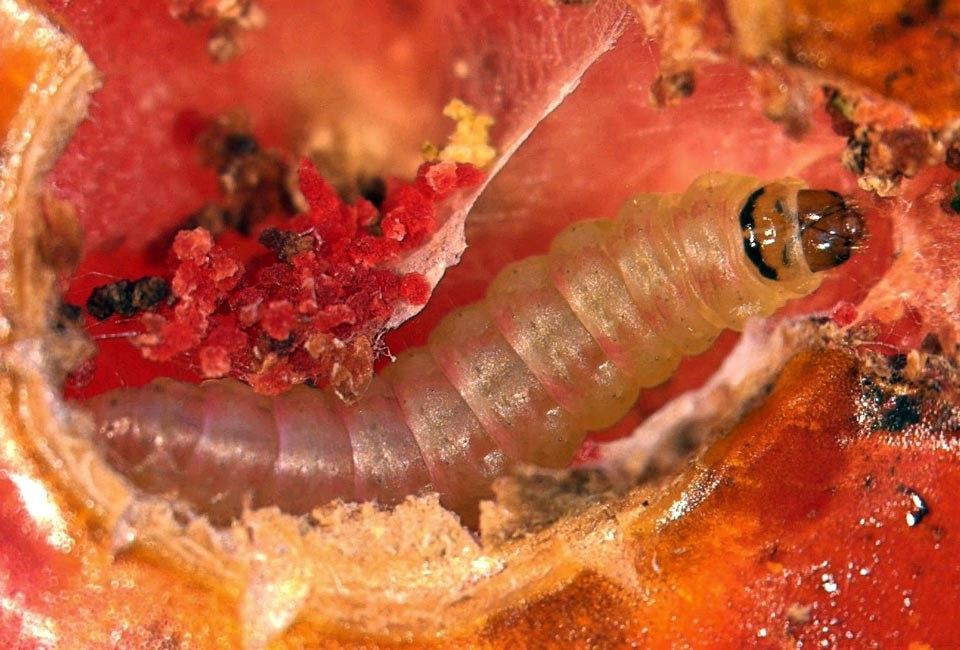
\includegraphics[width=0.8\linewidth]{./images/tuta_absoluta} \end{center}

The pest mainly presents nocturnal habits, and adults usually remain hidden during the day, showing greater morning-crepuscular activity with adults dispersing among crops by flying. Among a range of species within the Solanaceae, tomatoes ( \emph{Lycopersicon esculentum} Miller) appear to be the primary host of \emph{T. absoluta}.

\textbf{Management}

\begin{itemize}
\tightlist
\item
  Removing and destruction of infested plant parts. Tomato is the main host of the plant, but \emph{T. absoluta} also attacks other plants of the nightshade family -- Potato, eggplant, pepino, pepper and tobaccoo, including solanaceous weeds like \emph{Datura stramonium} and \emph{S. nigrum}.
\item
  Deep ploughing in spring season followed by solarization of field.
\item
  Continuous irrigation and inundating of field can help prevent pupation.
\item
  Crop rotation
\item
  Use of exclusion net (especially in nursery condition); Mesh size of less than 1.6 mm is recommended.
\item
  Use of sticky trap and light traps and yellow delta trap are useful in monitoring of \emph{T. absoluta} populations.
\item
  Para-pheromone TLM lure in Wota-T traps. The para-pheromone traps are used to monitor the adult moths. 5 Wota-T traps/ropani or 1 light trap/ropani.
\item
  Quarantine measures
\item
  Neem based pesticides (Neem raj), Jholmol botanicals
\item
  Imidacloprid, Emamectin benzoate (KINGSTAR, EMAR), Chlorantaniliprole (ALLCORA and CORAGEN) 18.5\% EC 1 ml per 3 ltr of water sprayed every 10-15 days, Spinosad (TRACER) 45\% SC 1 ml per 3 ltr water sprayed every 10-15 days, Chlorpyriphos and Cypermethrin.
\item
  Chlorantaniliprole, Spinosad and Flubendiamide (ryanoid class) all have waiting period of 7 days, while Emamectin benzoate, ranked as Moderately hazardous has waiting period of 10 days.
\item
  \emph{Bacillus thuringiensis kurstaki} (1\% WP 2 g per 1 ltr water sprayed every 7 days) have shown some efficiacy in controlling outbreaks of this moth. Similarly, \emph{Metarrhizium anisopliae} (\(1 \times 10^8\) CFU per gram ) 200-250 gm per ropani can be used for soil treatment.
\end{itemize}

\textbf{Monitoring of pest}

Crop damage should be monitored every two weeks. If noted abnormal minining in the leaf, with signs of mesophyll tissues being eaten and transparent veins exposed, suspect for presence of larvae of the pest. Tips of plant should show black massess, an indication of insect excreta. Fruits may show irregular strips of white coloration initially. In severe infestation, whole plant may appear as wilted. The larvae of Tuta will not enter diapause unless food is scarce. It is identifiable with characteristic pink colored body of 0.9 cm having half crescent rings like appearance in head.

\hypertarget{major-insects-of-guava}{%
\subsection{Major insects of guava}\label{major-insects-of-guava}}

\begin{itemize}
\tightlist
\item
  Fruit fly ( \emph{Dacus dorsalis})
\item
  Green shield scale ( \emph{Chloropulvinaria psidii})
\item
  Mealy bugs ( \emph{Ferrisia virgata}, \emph{Plannococcus citri})
\end{itemize}

\hypertarget{major-insects-of-jackfruit}{%
\subsection{Major insects of jackfruit}\label{major-insects-of-jackfruit}}

\begin{enumerate}
\def\labelenumi{\arabic{enumi}.}
\tightlist
\item
  Shoot and fruit borer ( \emph{Diaphania caesalis})
\item
  Giant mealy bug ( \emph{Drosicha mangiferae})
\end{enumerate}

\hypertarget{major-insects-of-litchi}{%
\subsection{Major insects of litchi}\label{major-insects-of-litchi}}

\begin{enumerate}
\def\labelenumi{\arabic{enumi}.}
\tightlist
\item
  Fruit borer ( \emph{Cryptophlebia illepida}, \emph{Rapala varuna}, \emph{Deudorix epijarbas}, \emph{Deudorix isocrates})
\item
  Fruit fly ( \emph{Bactrocera dorsalis})
\end{enumerate}

\hypertarget{fall-armyworm-faw}{%
\subsection{Fall armyworm (FAW)}\label{fall-armyworm-faw}}

The FAW life cycle is completed in 28-48 days depending on temperature and food availability but in laboratory conditions it has been observed to complete in 27-32 days at average daily temperature of \(27^\circ\) C. Heavy rainfalls are reported to break the life cycle of FAW. The insect is not reported to have the ability to diapause.

In Nepal, considering the low winter temperatures, migratory FAW are supposed to arrive if allowed by conducive environmental conditions.

\textbf{Life cycle}

\begin{enumerate}
\def\labelenumi{\arabic{enumi}.}
\item
  Egg: Creamy white or grey in color covered by light brown wool like material imparting a moldy appearance. The total eggs are dome shaped. The number of eggs per mass varies considerably but is often 100-200, and total egg production per female averages about 1500 with a maximum of over 2000. The female normally deposits most of her eggs during the first 4-5 days of life, but some oviposition continues to occur for upto 3 weeks. On average, adults live for 12-14 days. Egg continues unhatched for 2 days in warm laboratory conditions.
\item
  Larvae: The FAW has six larval instars. The first instar are whitish in color which later change into greenish color with black head. The larvae measures 30-35 mm long, and their color varies from brown, gray, yellowish, pinkish to greenish with granulated texture all over the body. The total larval period lasts 14-15 days in aforementioned laboratory conditions. Inverted `Y' shaped whitish marking is present on the head. The best identifying feature of the FAW is a set of four large spots (pinacular) that form a square on the upper surface of 8th segment of body. The late instar larvae also have three creamy yellow stripes on the dorsal surface which run in parallel manner from thorax to last abdominal segment. Larvae tend to hide themselves in the plant whorls during the sunny day.
\item
  Pupa: The FAW normally pupates in the soil at a depth of about 2-8 cm. The larvae constructs a loose cocoon by tying together particles of soil with silk. The pupae is reddish brown in color, measuring 14-18 mm in length and about 4.5 mm in width. Duration of pupal stage is 6-8 days in lab conditions.
\item
  Adult: Moths have a wingspan of 32-40 mm. Hind wings in both male and female are white with black lines on inner margins. Adult male moth of the insect has distinct markings on the forewings whereas markings on female forewings are not distinct. In male moth, the forewing generally is shaded gray and brown, with triangular white spots at the tip. Brown and oval shaped spot is present at the center of forewings. The forewings of females are less distinctly marked, ranging from a uniform grayish brown to a fine mottling of gray and brown. Adults are nocturnal, and are most active during warm, humid evenings. Duration of adult life cycle (as observed in laboratory conditions in Nepal) is 5-7 days.
\end{enumerate}

\textbf{Feeding behavior and damage}

The larvae can feed and damage entire plant including leaves, whorls, tassels, silk and ears. Early instars (1st and 2nd) feed by scrapping the leaf surface leaving the epidermis intact which results in the appearance of elongated papery windows of different size. They also bore into the whorl resulting into small pin holes.

Larvae of 3rd and 4th instars voraciously feed on foliage showing ragged and elongated holes on plant and size of holes increase with the growth of the larvae. Both 5th and 6th instars feed extensively and result in leaf area loss or defoliation overall. Severe feeding gives the appearance of maize plant that has been damaged by hail. After feeding, the larvae leave behind large amounts of moist saw dust like frass near the whorl and upper leaves.

In the maize crops' reproductive stage, taseel and ear are vulnurable to being bore into. The larvae can feed on kernels of ear affecting the yield, or cause quality deterioration due to mycotoxin contamination.

\textbf{List of pesticides that can be of potential use against FAW management}

\begin{enumerate}
\def\labelenumi{\arabic{enumi}.}
\tightlist
\item
  Azadirachta indica extracts (Margo NF), Azadirachtin (Agriguard, astan-killer, astha neem super-1, etc.)
\item
  Bacillus thuringiensis (Chandani-5 WP, Lipel, Mahastra-0.5 WP)
\item
  Chlorantranilipole 18.5\% SC (Allcora, Nicora gold, coragen, ferterra 0.4\% GR) at the rate 0.4 ml/ltr of water.
\item
  Emamectin benzoate (Aberkiller, Allclaim) 5\% SG at the rate 0.4 g/ltr of water.
\item
  Metarhizium anisopliae (Biocide manic, Emerald, Lalichakra, Pacer, Peak moti, Recharge, Varunastra)
\item
  Spinetoram (Delegate) 11.7\% SC at the rate 0.5 ml/ltr of water
\item
  Spinosad (Tracer) (Registered in 2019) 45\% SC at the rate 0.3 ml/ltr of water.
\end{enumerate}

\textbf{Monitoring of FAW}

\begin{enumerate}
\def\labelenumi{\arabic{enumi}.}
\tightlist
\item
  Trap selection: Suitable trap, it could be Funnel trap or Bucket trap
  2.Lure selection: Procure FAW specific pheromone lure, and store lures in a Refrigerator (\(4-5^\circ\)C); change the lure once every 4-6 weeks.
\item
  Trap placement and setup:
\end{enumerate}

\begin{itemize}
\tightlist
\item
  Establish the pheromone trap two weeks before planting at a height of approximately 1.25 meters from the ground level.
\item
  Place the trap in or next to the maize field
\item
  Install the trap from a long pole in a vertical orientation to prevent water entering into it and adjust the trap height to at least 30 cm above plant height.
\end{itemize}

\begin{enumerate}
\def\labelenumi{\arabic{enumi}.}
\setcounter{enumi}{3}
\tightlist
\item
  Install 3 traps per cluster at the distance of at least 50 meters apart.
\item
  Trap monitoring and recording: Weekly intervals throughout the season
\item
  Monitoring and crop phenology/stage
\item
  Area-wide and community-based approaches in terms of pheromone traps could be more effective than at the individual farm level
\item
  Record the weather record(temperature, humidity, rainfall, etc.),wherever possible.
\item
  Share and use the FAW monitoring data with extension agents.
\end{enumerate}

\textbf{Scouting pattern}

\emph{W pattern}

\begin{itemize}
\tightlist
\item
  Scouting in the field is done in a semi-systematic manner to determine the risk of yield depression associated with foliar feeding and density of small and large larvae. It is one of the approaches that follow a ``W'' pattern to cover the entire field.
\item
  While entering into the field for scouting at least two outer rows should be left. This is practiced to avoid border effect.
\item
  At every point, inspect 10-20 plants in a row or around the central plant of the point (in case of scattered planting).
\item
  Observe the signs in upper 3-4 leaves for damage or fresh frass carefully in each plant. Fresh frass indicates the presence of living larvae in the whorl.
\end{itemize}

\emph{Ladder pattern}

\textbf{IPM options for FAW}

\begin{itemize}
\tightlist
\item
  Seed and varieties (Seed treatment with Imidachlorpid 48\% FS at the rate of 4 ml per kg). This protects plant upto 2-3 after germination.
\item
  Select maize varieties with tight husk cover.
\end{itemize}

\textbf{Cultural management practices}

\begin{itemize}
\tightlist
\item
  Avoid late and staggered planting. Early planting often helps to escape the peak migration and incidence of FAW adults.
\item
  Use of recommended dose of manures and fertilizers.
\item
  Maintain adequate soil moisture for producing vigorous and healthy plants which can withstand pest infestation and damage.
\item
  Ploughing the field to a depth of 10 cm helps to expose FAW pupae to sunshine and natural enemies. Allow soil to be open for 2-3 after plowing for promoting this natural control.
\item
  Adopt push-pull technology incorporating Desmodium grass and other legume crops such as pigeonpea, beans, groundnuts as intercrops for push and border crop of Napier grass for pull.
\item
  Destroy crop residues after harvest for destroying sheltering eggs, larvae and pupae of FAW.
\item
  Practice crop rotation with alternate crops to minimize the attack of FAW.
\end{itemize}

\textbf{Mechanical control}

\begin{itemize}
\tightlist
\item
  Hand picking and crushing of FAW egg masses and young larvae (if found in field) or emmerse them into soap water.
\end{itemize}

\textbf{Biological control}'

\begin{itemize}
\tightlist
\item
  Natural enemies in field should be conserved with a provision of sheltering and pollen resourceful flowering plants around. Some naturally occurring biological organisms identified as effective control agents against FAW include:
\end{itemize}

\begin{enumerate}
\def\labelenumi{\arabic{enumi}.}
\tightlist
\item
  Predators (Earwigs, Ladybird beetles, Ground beetles, Assassin and flower bugs, predatory wasps, Spiders and Ants)
\item
  Parasitoids (\emph{Telenomus remus}, \emph{Chelonus insularis}, \emph{Cotesia marginiventris}, \emph{Trichogramma} spp., Fly parasitoids: \emph{Archytas}, \emph{Winthemia}, \emph{Lespesia})
\item
  Parasites and microbial pathogens (NPV, MNPV, BT, \emph{Nomuraea rileyi}, Entomopathogenic nematodes (\emph{Heterorhabditis, Steinernema}))
\end{enumerate}

\textbf{Botanicals and indigenous management options}

\begin{itemize}
\tightlist
\item
  Use of local botanicals (neem, hot pepper, titepati, timur and other plant extracts) act as antifeedant and repellant against FAW.
\item
  Sugary sprays, oil, ``fish soup'' or other materials can also be used to attract ants and wasps to the maize plants.
\end{itemize}

\textbf{Use of chemical pesticides}

\hypertarget{biochemistry-and-biotechnology}{%
\chapter{Biochemistry and biotechnology}\label{biochemistry-and-biotechnology}}

\hypertarget{plans-and-policies}{%
\chapter{Plans and policies}\label{plans-and-policies}}

\hypertarget{general}{%
\section{General}\label{general}}

\begin{itemize}
\tightlist
\item
  MOA has issued an ``Implementation Guidelines on PPS for Agriculture Development, 2055 (1998)'' to ensure common framework for implementation of pocket package strategy in order to carry out APP at field level. The guidelines have presented the pocket package program under two categories namely Crop production and Livestock production.
\item
  Agriculture fair is based on the concept of ``Seeing is believing''.
\item
  Department of Agriculture first broadcasted improved production technology in agriculture through radio for the first time in 2016 B.S.
\item
  Agriculture program broadcast over radio was stopped for a few years and later resumed back in 2023 Mangsir 20.
\item
  In group approach of extension is used in convincing a farmer to use a technology when s/he has been made aware of it through mass media approach.
\end{itemize}

\hypertarget{national-tea-policy-2000}{%
\section{National tea policy, 2000}\label{national-tea-policy-2000}}

\begin{itemize}
\tightlist
\item
  GoN approved and implemented National Tea Policy, 2000 as per intention of National Tea and Coffee Development Board Act, 1992 for:

  \begin{itemize}
  \tightlist
  \item
    Income generation (enhancing employment, earning foreign currency)
  \item
    Participation in private sector in production, processing and commercial transaction through systematic and sustainable utilization of resources in country.
  \end{itemize}
\item
  Working policies:
  A. Production and processing

  \begin{itemize}
  \tightlist
  \item
    Banks to provide priority credit
  \item
    Upto 80\% loan of total project cost to registered tea plantation industry
  \item
    7 years grace for orthodox tea and 5 years for green tea on loan in hills and terai respectively.
  \item
    Interest on loan not capitalized in grace period
  \item
    Income tax not levied within grace period
  \item
    Interest and principal to be fully paid up within 10 years from the end of grace period
  \item
    Exemption of 75\% on land registration fee
  \item
    Land revenue exemption
    B. Market and trade promotion
    C. Institutional arrangement
    D. Manpower development
    E. Development and promotion of auxillary industries
  \end{itemize}
\end{itemize}

\hypertarget{national-agricultural-policy-2004}{%
\section{National agricultural policy, 2004}\label{national-agricultural-policy-2004}}

Vision

\begin{itemize}
\tightlist
\item
  To bring about an improvement in the standard of living through a sustainable agricultural development to be achived by transforming the current subsistence oriented farming system into a commercial and competative farming system.
\end{itemize}

Objectives

Broad

\begin{itemize}
\tightlist
\item
  To ensure food security and poverty alleviaion by achieving a high and sustainable economic growth through commercial and competative farming system.
\end{itemize}

Specific

\begin{itemize}
\tightlist
\item
  Agricultural production and productivity shall be increased
\item
  The bases of a commercial and competative farming system shall be developed and made competative in regional and world markets
\item
  Natural resources, as well as the environment and biodiversity shall be conserved, promoted and properly utilized
\end{itemize}

Policies

Objective 1

\begin{itemize}
\tightlist
\item
  Increasing of agricultural production and productivity

  \begin{enumerate}
  \def\labelenumi{\arabic{enumi}.}
  \tightlist
  \item
    Utilize local potentialities, comparative advantage and special opportunities; Ensure development, extension and utilization of agricultural technology; Commercialization and diversification of agriculture
  \item
    Scientific land use system
  \item
    Irrigation, agricultural roads, rural electrification and appropriate agriculture technology development and epansion
  \item
    Pocket development of HVAP
  \item
    Entrust local body for formulating, implementing and monitoring agricultural plans suitable to local needs and priorities. Conditional basis of grant.
  \item
    Multi-district projets to promote agricultural produciton and enterprises operated and suppored at implementation level through central departments and directorates.
  \item
    Farmer's group appraoch for on-site extension service
  \end{enumerate}

  \begin{itemize}
  \tightlist
  \item
    Agriculture and frest colleges to extend agriculture technologies through package programs
  \item
    IT and mass communication development
  \end{itemize}

  \begin{enumerate}
  \def\labelenumi{\arabic{enumi}.}
  \setcounter{enumi}{7}
  \tightlist
  \item
    National agricultural resource centres for high quality inputs
  \end{enumerate}

  \begin{itemize}
  \tightlist
  \item
    based on development regions and geo-graphical subdivisions
  \item
    NARC to be converted to integrated centre
  \end{itemize}

  \begin{enumerate}
  \def\labelenumi{\arabic{enumi}.}
  \setcounter{enumi}{8}
  \tightlist
  \item
    Participatory and competative agricultral research and development system promotion
  \end{enumerate}

  \begin{itemize}
  \tightlist
  \item
    Technology exchange encouraged between organizations
  \end{itemize}

  \begin{enumerate}
  \def\labelenumi{\arabic{enumi}.}
  \setcounter{enumi}{9}
  \tightlist
  \item
    Private and foreign investment in agriculture research and development encouraged
  \item
    Input supply monitoring and regulating guarenteed
  \item
    Surveillance system to assess impact of excessive rains, droughts and calamities.
  \item
    Emphasis on farmer's training programs
  \item
    Linkage of agricultural production and enterprises' return to ensure agriculture credit flow.
  \item
    Establishment of agriculture and forestry university. Quality of agriculture human resource to be increased by arranging cooperation and exchange of technicians and experts among universities/colleges, agriculture research centre and national agriculture resource center.
  \item
    System development for collecting, analyzing and projecting data required for formulation of plans, determining policies and carrying out monitoring and evaluation of activities related to agriculture sector shall be strengthened.
  \item
    Women's participation in all fields of agriculture upto 50\%
  \item
    Resource poor farmers (with less than 4 hectares of land) will be identified and classified.
  \end{enumerate}
\end{itemize}

Objective 2

\begin{itemize}
\tightlist
\item
  Special facilities for target groups: For farmer's having less than 0.5 hectares and unirrigated lands, dalit and utpidit classes of farmers and other marginal farmers

  \begin{enumerate}
  \def\labelenumi{\arabic{enumi}.}
  \tightlist
  \item
    Opportunity of gaining access to lands
  \end{enumerate}

  \begin{itemize}
  \tightlist
  \item
    Legal ceilings on landholdings and exemptions
  \item
    Progressive taxation
  \item
    Legal provision for contractual farm lands.
  \end{itemize}

  \begin{enumerate}
  \def\labelenumi{\arabic{enumi}.}
  \setcounter{enumi}{1}
  \tightlist
  \item
    Land bank establishment
  \end{enumerate}

  \begin{itemize}
  \tightlist
  \item
    Local body as information provider
  \item
    Concessional loans
  \end{itemize}

  \begin{enumerate}
  \def\labelenumi{\arabic{enumi}.}
  \setcounter{enumi}{2}
  \tightlist
  \item
    Forest upgradation and other land will be handed to the traget communities under lease.
  \item
    Special facilities to target groups to build and install infrastructures: small irrigation (pedal pumps, power pumps, sprinklers, drips and water harvesting ponds)
  \item
    Utilization of means to increase production and income to mitigate food deficit. Network for food mobilization development.
  \item
    Government services based on priority from food security viewpoint.
  \item
    Food safety nets development for farmers with less than 0.5 hectares of land.
  \end{enumerate}
\end{itemize}

Objective 3

\begin{itemize}
\tightlist
\item
  Development of commercial and competative farming system

  \begin{enumerate}
  \def\labelenumi{\arabic{enumi}.}
  \tightlist
  \item
    Large production pockets, priority for comparative advantage products. Technology and technical sevices as well as infrastructure mobilized in integrated manner.
  \item
    Local production of food grains will be encouraged under food supply programme
  \item
    Double track management system will be adopted in government farms and centres
  \item
    Livestock insurance programmes extension. Poultry insurance and HVAP and seed crops insurance.
  \item
    Organic farming will be encouraged; certification support
  \item
    Production of hybrid seeds and improved seeds will be encouraged, GMOs will be regulated.
  \item
    Traditional, local original agriculture products and technologies will be registered and promoted.
  \item
    Agriculture training classification
  \end{enumerate}

  \begin{itemize}
  \tightlist
  \item
    Capacity improvement training for agriculture workers and farmers
  \item
    Enterprise promotion training
  \end{itemize}

  \begin{enumerate}
  \def\labelenumi{\arabic{enumi}.}
  \setcounter{enumi}{8}
  \tightlist
  \item
    Training educated but unemployed youths
  \item
    Local production, sale and distribution of improved agriculture resource inputs (seeds, plants, saplings, breeds, fingerlings, etc.) and manure, insecticides, pesticides, regulated and quality control.
  \end{enumerate}

  \begin{itemize}
  \tightlist
  \item
    Private agriculture lab services will be regulated and accreditated
  \item
    High quality product processing facilites and services will be offered
  \end{itemize}

  \begin{enumerate}
  \def\labelenumi{\arabic{enumi}.}
  \setcounter{enumi}{10}
  \tightlist
  \item
    Agriculture and livestock quarentine services will be systematized and strengthened in order to ensure the production of high quality agriculture products and raise their credibility in local and external markets.
  \item
    Participation of local bodies will be strengthened in determining, controlling, certifying, and regulating standards of food stuffs.
  \item
    Regulatory services will be upgraded as per international treaties and agreements and the national requirements.
  \item
    Promotion of cooperative based agriculture industries and enterprises
  \item
    Mobilize agriculture industry and enterprise promotion board
  \end{enumerate}

  \begin{itemize}
  \tightlist
  \item
    To analyze and provide outlet to complaints and suggestions
  \end{itemize}

  \begin{enumerate}
  \def\labelenumi{\arabic{enumi}.}
  \setcounter{enumi}{15}
  \tightlist
  \item
    Commodity and subject specific policies equipped with incentives developed in order to attract cooperative and private sectors to make investments in commercial production, processing and marketing
  \item
    Agricultural industry development policy formulation
  \end{enumerate}

  \begin{itemize}
  \tightlist
  \item
    Interlink agriculture research + production + processing industries + internal and external export markets
  \end{itemize}

  \begin{enumerate}
  \def\labelenumi{\arabic{enumi}.}
  \setcounter{enumi}{17}
  \tightlist
  \item
    Free-based agricultural technology extension services in areas of commercial agricultural production
  \item
    Private sectors engaged to operate suitable farms/centers through contract lease agreements.
  \item
    Developing and extending market information system and disseminating such information shall be carried out in private + cooperative + local bodies partnership
  \item
    Collection centres close to production centres (Hat bazzars, well equipped wholesale and seasonal markets as well as private cooperatives)
  \item
    Agriculture enterprise promotion board to provide capital and incentives/facilities to industries and enterpreneurs for:
  \end{enumerate}

  \begin{itemize}
  \tightlist
  \item
    import substitution
  \item
    export promotion
  \end{itemize}

  \begin{enumerate}
  \def\labelenumi{\arabic{enumi}.}
  \setcounter{enumi}{22}
  \tightlist
  \item
    Cooperative promotion of potential farmer groups and enterprenuers by mobilizing and promoting local small capital and other resources
  \end{enumerate}

  \begin{itemize}
  \tightlist
  \item
    Rural cooperatives as local delivery points
  \end{itemize}
\end{itemize}

Objective 4

\begin{itemize}
\tightlist
\item
  Conservation, promotion and utilization of natural resources and environment

  \begin{enumerate}
  \def\labelenumi{\arabic{enumi}.}
  \tightlist
  \item
    Impact minimization of agro-chemicals
  \item
    Organic fertilizer promotion
  \item
    Gene banks and insitu conservation. Participatory biodiversity parks
  \item
    Biodiversity conservation, promotion and utilization to improve condition of degraded forests and natural reservoirs.
  \item
    Conservation oriented farming system
  \end{enumerate}

  \begin{itemize}
  \tightlist
  \item
    Watershed management through local participation
  \item
    Soil erosion control through local participation
  \end{itemize}

  \begin{enumerate}
  \def\labelenumi{\arabic{enumi}.}
  \setcounter{enumi}{5}
  \tightlist
  \item
    Checking cultivable land fragmentation and ensure scientific mangement
  \end{enumerate}
\end{itemize}

Objective 5

\begin{itemize}
\tightlist
\item
  Implementation and monitoring arrangement

  \begin{enumerate}
  \def\labelenumi{\arabic{enumi}.}
  \tightlist
  \item
    Participatory involvement of stakeholders in process of formulating, monitoring and evaluating plans connected with agriculture sector from local to central level.
  \item
    Role of national agricultural development board (Central agriculture development committee and Regional agriculture development committee) devolution for policy implementation to local bodies (VDCs and DDCs) to ensure formulation, implementation, monitoring and evaluation of plans in accordance to LSGA, to:
  \end{enumerate}

  \begin{itemize}
  \tightlist
  \item
    DADC (District agriculture development committee) with technical feedbacks to CADC and RADC
  \item
    ADC (Village level ADCs) with technical feedbacks to CADC and RADC.
  \end{itemize}

  \begin{enumerate}
  \def\labelenumi{\arabic{enumi}.}
  \setcounter{enumi}{2}
  \tightlist
  \item
    Concerned ministries shall implement this policy on their related sectors
  \end{enumerate}

  \begin{itemize}
  \tightlist
  \item
    NADC to monitor the implementation on national level
  \item
    Strategies, programs and responsible bodies of related matters may be implemented by concerned ministries upon approval.
  \end{itemize}
\end{itemize}

\hypertarget{general-knowledge-multiple-choice-agriculture}{%
\chapter{General Knowledge Multiple Choice: Agriculture}\label{general-knowledge-multiple-choice-agriculture}}


\includepdf[pages=2-,pagecommand={},width=1.2\textwidth]{./latex-compiled/main.pdf}

  \bibliography{bibliography/vegetable.bib,bibliography/bib.bib}

\end{document}
